\documentclass[12pt, a4paper, twoside]{memoir}
\usepackage{tikz} % Figures
\usepackage{layout} % Margin
\usepackage{setspace} % Double space
\usepackage [top=3cm, bottom=2cm, left=2cm, right=2cm]{geometry} % Margin
\usepackage{graphicx} % Images
\usepackage{caption}
\usepackage{subcaption}
\usepackage{float}
% To write formulas
\usepackage{amsfonts}
\usepackage{amsmath}
\usepackage{amssymb}
\usepackage{mathrsfs}

% Plot
\usepackage{pgfplotstable}
\usepackage{pgfplots}
\pgfplotsset{compat=newest}

\usepackage{hyperref}

\usepackage{relsize}
\usepackage{helvet}

% Commands
\newcommand{\newpar}{\vskip 0.2in \noindent}
\newcommand\tab[1][1cm]{\hspace*{#1}}

\makeevenhead{headings}{\sffamily\thepage}{}{\sffamily\leftmark} 
\makeoddhead{headings}{\sffamily\rightmark}{}{\sffamily\thepage}
\makeoddfoot{plain}{}{}{} % Pages chapitre. 
\makeheadrule{headings}{\textwidth}{\normalrulethickness}
\chapterstyle{dash}
\renewcommand{\chaptername}{\relax}
\renewcommand{\chaptitlefont}{ \sffamily\bfseries \LARGE}
\renewcommand{\chapnumfont}{ \sffamily\bfseries \LARGE}
\setsecnumdepth{subsection}
\renewcommand{\abstracttextfont}{\normalfont}

\pagestyle{headings}

\pretitle{\HUGE\sffamily \bfseries\begin{center}} 
\posttitle{\end{center}}
\preauthor{\LARGE \sffamily \bfseries\begin{center}}
\postauthor{\par\end{center}}

\newcommand{\jury}[1]{\gdef\juryB{#1}} 
\newcommand{\juryB}{} 
\newcommand{\session}[1]{\gdef\sessionB{#1}} 
\newcommand{\sessionB}{} 

\renewcommand{\maketitlehookd}{\vfill{}\large\par\noindent \begin{center}\juryB \bigskip\sessionB\end{center}\vspace{-1.5cm}}

\renewcommand{\maketitlehooka}{\vspace{-1.5cm}\noindent \includegraphics[height=14ex]{img/l_uga}\hfill\raisebox{0ex}{\includegraphics[height=14ex]{img/l_ensimag}}\\
\bigskip
\begin{center} \large
	\textsc{Master Operation Research, Combinatorics and Optimization ORCO} \\ 
	Master of Science in Computer sciences at Grenoble \\
	Master Computer sciences / Master Applied mathematics
\end{center}\vfill}
% End of title page formatting
%%%%%%%%%%%%%%%%%%%%%%%%%%%%%%%%%%%%%%%%%

%%%%%%%%%%%%%%%%%%%%%%%%%%%%%%%%%%%%%%%%%
% Personalisation
	\title{\textsc{Decision Support System for carpooling to reduce car traffic in Grenoble area}}%\\\vspace{-1ex}\rule{10ex}{0.5pt} \\sub-title} 
	\author{Romain NAVARRO}
	\date{June, 28th 2018}
	\jury{
		\begin{tabbing}
			\tab \=Research proj\=ect performed at G-SCOP, under the supervision of:\\
			\> \> \textsc{Prof.} \=Van-Dat \textsc{CUNG}, G-SCOP\\\medskip
			\>Defended before a jury composed of:\\
			\> \> \textsc{Prof.} \>Nadia \textsc{BRAUNER}\\
			\> \> \textsc{Prof.} \>Van-Dat \textsc{CUNG}\\
			\> \> \textsc{Dr.} \>Vassilissa \textsc{LEHOUX}\\
			\> \> \textsc{Prof.} \>Matej \textsc{STEHLIK}\\
		\end{tabbing}
	}
\session{$June$\hfill 2018}

\begin{document}
	\frontmatter\begin{titlingpage}\maketitle\end{titlingpage}
	% ABSTRACT
	\begin{abstract}
		\noindent The problem of carpooling is a problem of satisfaction for users who would like to have as little inconvenience as possible. We can cite some of the inconveniences of current carpooling systems, such as inadequate schedules, long detours, or not enough flexibility, home-to-work trips.
		\newpar
		We have studied the possibilities of minimizing these inconveniences, and here are the main points:\newline 
		Our system offers a daily solution to avoid long-term commitment problems and to have more flexibility.\newline 
		Our system allows users to have different places of work, either if the user does not have a fixed place of work, or if he wants to go somewhere before going home. The user can also have several places of residence within a single day, if he does not want to return to the same place. Thus, the user can have one origin and destination in the morning, then another origin and destination in the evening.
		\newpar
		Our objective is to create user groups to minimize the distance travelled by users while maximizing vehicle occupancy. \newline
		Furthermore, we will study the impact of these inconveniences on the possible solutions, by varying the possible advance at work, as well as by varying the authorized detour lengths.
		\begin{center}
			{\bfseries Key-words}: optimization - multi-destination daily carpooling problem - home to work - return management
		\end{center}
	\end{abstract}

	% TABLE OF CONTENTS
	\cleardoublepage
	\renewcommand{\contentsname}{Table of contents}
	\mainmatter
	\tableofcontents
	
	%%%%%%%% %%%%%%%% %%%%%%%%
	%%%%%%%% INTRODUCTION %%%%%%%%
	%%%%%%%%% %%%%%%%% %%%%%%%
	\cleardoublepage
	\chapter{Introduction}
	
	Carpooling is subject to intense research, yet many users continue to take their personal car. Private car use accounts for the largest part of kilometers traveled and is considered one of the most important contributors to air pollution \cite{laucontributions2008}. Promoting eco-friendly transportation modes (such as public transportation, bicycle, walking, or carpooling) is becoming more and more frequent. However, even with increasing environmental awareness and concern, many road users are still car-dependent, either by choice or constrained by circumstances \cite{stradeterminants2007}. These car-dependent users therefore have no access to any other means of transportation. The carpooling is the most suitable alternative \cite{delhommecomparing2016}.
	\newpar 
	Now we'll see what carpooling is.
	
	% OBJECT
	\section{Definition of the carpooling}\label{sec:The kinds of carpooling}
	We will start by defining what carpooling is. Definitions vary considerably in the literature, nevertheless we can form a general definition of the idea behind these terms. Carpooling is the use of private cars, unlike car-sharing which uses cars assigned to a system. We can define it by forming groups of people, say pools, each sharing the same car. These pools are on average formed by more than one person per car. The people of the pool participate, by various means, in the expenses generated by the trips.\newline
	There are many systems for connecting people, such as websites that ask users who go from one city to another to enter their route, or universities and companies themselves forming groups of people based on their own data.
	\newpar
	We'll 
	
	% ISSUES
	\section*{Issues of the carpooling}
	
	Carpooling has advantages for the city and for users, we can cite the reduction of traffic jams, pollution and accidents. It also leads to freer parking, savings and more user-friendliness \cite{berlingeriograal2017}.
	\newpar
	By analyzing a few articles, we have compiled lists, representing the advantages and disadvantages for carpool users, as well as the advantages for companies that their employees make the trip together \cite{huangmodels2000} \cite{onwubolunew2004} \cite{yanoptimization2011} \cite{bruglieripoliunipool:2011}.
	\begin{tabbing}
		{\bfseries Advantages for the user:}\\
		\tab \= Split\=ting of expenses \\
		\> Compared to public transports \> \\
		\> \> No waiting \\
		\> \> Less time \\
		\> \> No walk \\
		\> Less need to get a special car to work \> \\
		\> Reduce traffic congestion / traffic volumes \> \\
		\> Reduce noise levels \> \\
		\> Reduce air pollution (vehicles emission) \> \\
		\> Fewer accidents \> \\
		\> Fuel savings \> \\
		{\bfseries Disadvantages for the user:} \\
		\> Flexible hours: not convenient \\
		\> \> Spread of flextime \\
		\> Increase travel time \\
		\> \> Pick up \\
		\> \> Deliver \\
		\> \> Mutual waiting \\
		\> Loss of independence \\
		\> Loss of privacy \\
		\> Loss of self-reliance \\
		\> Anonymity of the vehicle creates a more comfortable social climate \\
		\> \> Public cars \\
		{\bfseries Advantages for the companies: }\\
		\> Maximize the use of employee parking \\
		\> Sociability between the employees \\
		\> Reduce stress in driving to work \\
		\> Improve the company image \\
	\end{tabbing}
	
	\noindent From this list, we can mention the disadvantages on which we will work, namely flexible working hours, travel time and user independence. \newline
	Still according to the articles, \cite{huangmodels2000} \cite{onwubolunew2004} \cite{yanoptimization2011} \cite{bruglieripoliunipool:2011} we can separate the \textbf{issues} into different categories:
	\newpar
	\textbf{Environmental} issues related to reducing the consumption of non-renewable energy (oil) and reducing greenhouse gas emissions.
	\newpar
	\textbf{Structural} issues related to the reduction in the number of vehicles on the roads and developments related to parking. Carpooling facilities are becoming more common, such as free outdoor parking for carpoolers, near transportation or meeting points for carpoolers. If some structures are no longer useful, such as a three-lane road, the city would build new structures for the sustainable development of the city, such as green spaces and cycle paths.
	\newpar
	\textbf{Economic} issues with the reduction of the cost of road maintenance for the city, and the cost of vehicle wear and tear for the user.
	\newpar
	With the collection of data on carpooling, we would observe traffic flows in order to implement new solutions, such as the development of a new subsidiary road in a place with many companies. There are other viable solutions, such as traffic light management or the creation of new roundabouts. 
	\newpar
	We have the background to define the context in which the subject of our report is set.

	% CONTEXT
	\section*{Context of the report}
	In this report, we are interested in carpooling in France, more particularly in the case of the Grenoble conurbation and its surroundings. The French use carpooling less than their European neighbours, the reasons they give are that they have better \textbf{control of their schedule}, they arrive \textbf{on time at work}, and it is \textbf{faster} \cite{delhommecomparing2016}. In response we have set up some ways to take into account these reasons.
	\newpar
	With regard to the \textbf{control of the schedule}, we decided to make a system based on \textbf{daily carpooling}, to be able to change the schedule of the next day. \newline
	We also manage the \textbf{return trip from work}, to be closer to the user's schedule. \newline
	We also allow the user to have \textbf{different origins and destinations in the morning and evening}. \newline
	Thanks to these specificities, users benefit from greater flexibility and a more respected schedule.
	\newpar
	Regarding the arrival \textbf{on time at work}, we set up a \textbf{time window} to \textbf{not be too ahead at work}: it is a time window between zero and a fixed time. We will explain it more in detail later. \newline
	The return trip has a similar time window system, in order to \textbf{avoid the user to wait too long} after finishing his job. 
	\newpar
	Finally, we set up a management of the travel time, to define either a \textbf{percentage of the trip allowed time}, or a \textbf{fixed time}, or \textbf{both}. \newline
	For example, on a user's 100-kilometre home-work trip, if we allow a 10 per cent detour and add 10 kilometres of detour, the result will be 100 kilometres plus 10 kilometres plus 10 kilometres, which is 120 kilometres of travel allowed for that user. 
	\newpar
	To reduce traffic congestion in Grenoble, the study focuses on the home-work commute. 
	\newpar
	We will give more details, with illustrations of examples in the presentation of the problem \ref{fig:same workplace}. To understand the current situation, we will talk about smartphone applications that are currently on the French market. 
	
	% Existing applications
	\section*{Existing applications}
	
	It is important to talk about existing applications for home-to-work trip because we need to understand the specificities of existing systems.\newline
	The carpooling market from one city to another is owned by BlaBlaCar \cite{dionneblablacar2018}.However, when it comes to carpooling from home to work, their subsidiary BlaBlaLines has competition. We will quickly see what characterizes each of the flagship \textbf{applications} of the moment.
	\newpar
	\textbf{BlaBlaLines} links users according to their schedule, allowing a detour of at most fifteen minutes for a trip. Ultimately, they would like to set up a system of "lines" on busy roads, where drivers receive matching requests to their schedule and their road, and have the choice to accept or ignore it \cite{noauthorblablalines2017}. Their goal is to have as much flexibility as possible with no long-term commitment .
	\newpar
	\textbf{Klaxit} mainly relies on partnerships with communities and companies. Its principle is to find regular close carpoolers \cite{ARNULFKlaxit2018}. It fits with people who often have the same hours within the same company.
	\newpar
	\textbf{Karos} combines car and public transport. In addition, the application will learn from your usual routes to offer you matching carpoolers \cite{noauthorkaros2016}.
it fits with people who periodically do the same circuit.
	\newpar
	Each of these applications have theirs advantages and theirs disadvantages, with customer types specific to each. However, the market seems to be able to offer more in view of the very low occupancy rate per car during home-to-work journeys \cite{noauthoroccupancy2008}. \newline
	In addition, the French government is implementing the reimbursement of home-to-work journeys during strike periods, which is beneficial for both users and applications \cite{noauthorgreve2018}.
	
	\section{
	
	\newpar
	Having the necessary background for understanding the report, we will see the order of chapters in the next section.
	% Conduct of the project
	\section*{Conduct of the project}
	Here is an introduction to the chapters and the guideline followed throughout the report.
	\newpar
	First, the positioning in the literature of our subject will be highlighted. The existing will be presented, as well as the contribution to the research of our problematic.\newline
	Secondly, the problem will be explained in detail, with illustrations of the original concepts that we bring in relation to the existing.\newline
	Third, the data model and the mathematical model used in this internship will be presented. We will explain the constraints and data used, in order to understand the resolution method used.\newline
	Finally, we will see how the data was generated and/or recovered. We will initiate the scenarios, the expected results, then we will present and analyze the results obtained.
	
	%%%%%%%%%%%%%%%% STATE OF THE ART %%%%%%%%%%%%%%%%
	\cleardoublepage
	\chapter{State of the art}
	
	Carpooling is a vast and varied field, and the existing articles concern as much specific points as general cases.
	\newpar
	First, we will define the class of the problem.
	
	% Class of the problem
	\section{Class of the problem}
	In order to better understand the state of the art, we will define the problem classes that best correspond to our problem:
	\begin{figure}[H]
		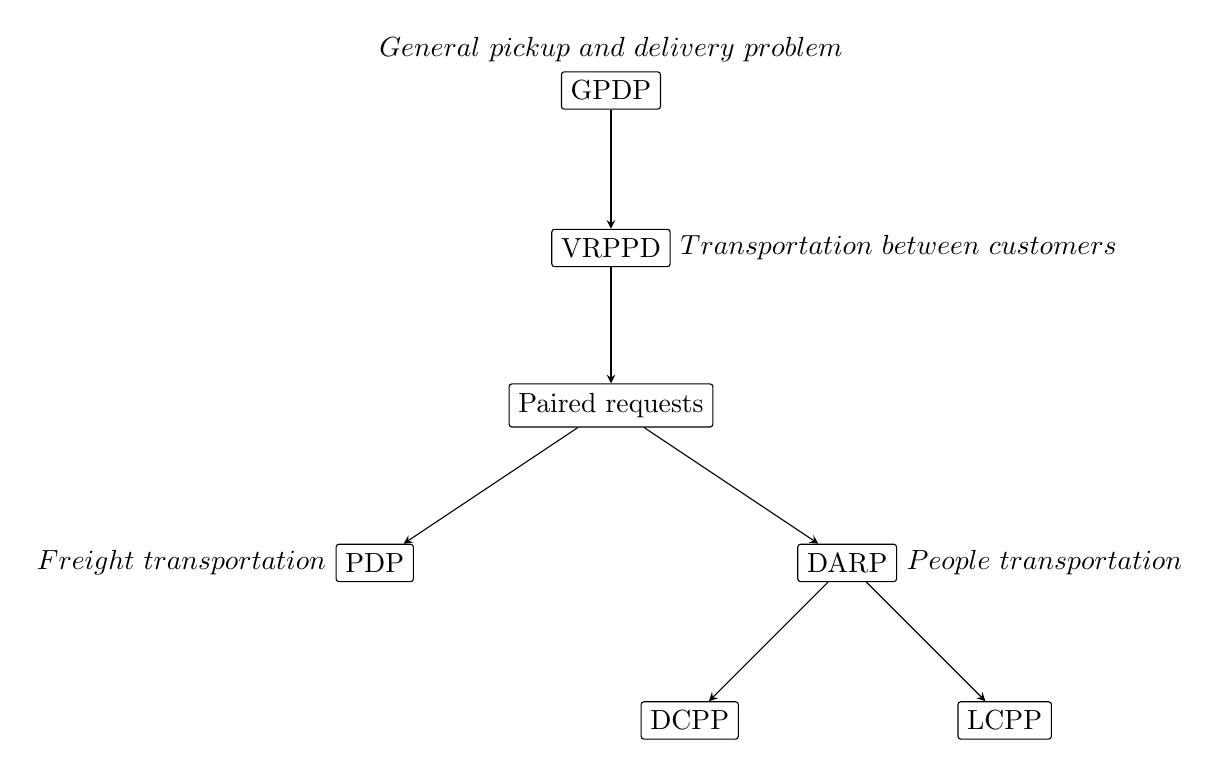
\begin{tikzpicture}
			\node[draw, rectangle, rounded corners=1, label=above:{$General$ $pickup$ $and$ $delivery$ $problem$}] (GPDP)at(0, 6) {GPDP};
			\node[draw, rectangle, rounded corners=1, label=right:{$Transportation$ $between$ $customers$}] (VRPPD)at(0, 4) {VRPPD};
			\node[draw, rectangle, rounded corners=1, label=above:{$$}] (PR)at(0, 2) {Paired requests};
			\node[draw, rectangle, rounded corners=1, label=left:{$Freight$ $transportation$}] (PDP)at(-3, 0) {PDP};
			\node[draw, rectangle, rounded corners=1, label=right:{$People$ $transportation$}] (DARP)at(3, 0) {DARP};
			\node[draw, rectangle, rounded corners=1, label=above:{$$}] (DCPP)at(1, -2) {DCPP};
			\node[draw, rectangle, rounded corners=1, label=above:{$$}] (LCPP)at(5, -2) {LCPP};
			\draw[->, >=stealth] (GPDP) -- (VRPPD);
			\draw[->, >=stealth] (VRPPD) -- (PR);
			\draw[->, >=stealth] (PR) -- (PDP);
			\draw[->, >=stealth] (PR) -- (DARP);
			\draw[->, >=stealth] (DARP) -- (DCPP);
			\draw[->, >=stealth] (DARP) -- (LCPP);
		\end{tikzpicture}
	\caption{Problem classes tree}
	\label{fig:Problem classes tree}
	\end{figure}
	
	Figure \ref{fig:Problem classes tree} is the problem classes tree, each of these problems defined below. The definitions are inspired by \cite{parraghsurvey2008} and \cite{guometaheuristics2012}.
	
	\begin{itemize}
		\item \textsc{The General Pickup and Delivery Problem} \textbf{GPDP}: \newline
		\tab There is a set of routes built to satisfy the transport requests. \newline
		\tab A fleet of vehicles is available to get to the roads, where each vehicle has a capacity, a starting point and an ending point. \newline
		\tab Each request specifies the size of the load to be transported, the origin and destination of that load. 
		\item \textsc{Vehicle Routing Problem with Pickup and Delivery} \textbf{VRPDP}: \newline
		\tab Contraction between Vehicle Routing Problem \textbf{VRP} and Pickup and Delay Problem \textbf{PDP}.\newline
		\tab It concerns the transportation to customers, and between customers. 
		\item \textsc{Vehicle Routing Problem} \textbf{VRP}: \newline
		\tab Either the origin or the destination of the vehicles are depots.
		\item \textsc{Pickup and Delay Problem} \textbf{PDP}: \newline
		\tab Requests specify a single origin and a single destination, and vehicles leave a repository and return to a repository. 
		\item \textsc{Dial-A-Ride Problem} \textbf{DARP}: \newline
		\tab Pickup and delivery used for people transportation. \newline
		\tab Take into account the user inconveniences.\newline
		\tab Users formulate transport requests from an origin (pick-up point) to a destination (drop-off point) \cite{yanoptimization2011}. 
		\item \textbf{PDP}\textsc{ and} \textbf{DARP} \textsc{are} \textbf{Paired}: \newline
		\tab Each request has an origin-destination pair.
	\end{itemize}
	\textbf{DCPP} and \textbf{LCPP} \hyperref[sec:The kinds of carpooling]{[ref: Introduction]} are variants of the \textbf{DARP}, where each person taking his car is a deposit of his vehicle.
	\newpar
	All these problems can be treated with the management or not of time windows. In the case of \textbf{DARP}, and therefore \textbf{DCPP} and \textbf{LCPP}, this management is included. \newline
	We manage people daily with our system, so \textbf{we are in the case of a Daily CarPooling Problem DCPP}.
	\newpar
	Now that we have defined problem classes, let's speak about resolution methods: There are either heuristics methods, or exact methods, or a combination of both(hybrid).
	
	% Resolution methods
	\section{Resolution methods}
	
	In this section will be presented some existing articles about the subject.
	
	\subsection{Exact methods}
	
	Exact methods are objectives and constraints giving an exact solution on a linear program. \newline 
	Mr. Cordeau \cite{cordeaubranch-and-cut2006} \cite{yanoptimization2011} is solving a DARP with a Branch-and-Cut linear program. $MDCPP$ is an extension designating the consideration of multi-destination, there are several places of work instead of one, and Mr. Guo \cite{guometaheuristics2012} presents it in his chapter 5. In a survey\cite{parraghsurvey2008} the differences in constraints between a PDP and a DARP will be shown.
	
	\subsection{Heuristics}
	The management of many data is not possible for problems that are not solvable in a polynomial time. This is why heuristic algorithms have been designed to obtain viable solutions on large instances. 
	\newpar
	\textsc{Genetic}\newline
	The principle of Genetic Algorithms \textbf{GA} is based on three phases:\newline
	\textbf{Natural selection}: Selection of individuals most likely to obtain the best results. \newline
	\textbf{Crossing}: Crossing of individuals with a probability between $0$ and $1$. \newline
	\textbf{Mutation}: Probability of mutation of an individual between $0.001$ and $0.01$. \newline
	Mr. Huang uses this algorithm in cloud computing which consists in harnessing the computing or storage power of remote computer servers via a network \cite{huanggenetic-algorithm-based2015}. \newline
	There are variants to these algorithms, such as GGA and AGA: \newline
	Guided Genetic Algorithm \textbf{GGA} is a Genetic Algorithm Oriented for Selection and Crossing \cite{guometaheuristics2012}. In Multi-Agent Self-Adaptive Genetic Algorithm \textbf{AGA}, each agent shares its progress with other agents. Learning mechanisms guide the genetic structure in order to have more appropriate choices. \cite{guometaheuristics2012} 
	\newpar
	\textsc{Tabu}\newline
	The principle of Tabu Algorithms \textbf{TA} is to find local minimums, save their position in a queue so as not to return to an already explored position. It is used in particular by Mr. Gendreau \cite{gendreautabu1996}, by Mrs. Li and Lim \cite{limetaheuristic2003}, and by Mr. Cordeau \cite{cordeautabu2003}. 
	\newpar
	\textsc{Simulation Based Approach}\newline
	Use the K-averaging algorithm to form groups \cite{correiaconceptual2009}.
	\newpar
	\textsc{Neighborhood Search Variable}\newline
	Search among "far-off" for the best local solution \cite{polacekvariable2004}.
	\newpar
	\textsc{Clustering Ants Colony}\newline
	Forms clusters during the construction of the "paths" of agents (ants) \cite{mazzeoant2004} \cite{guometaheuristics2012}.
	
	\subsection{Hybrid methods}
	Hybrid methods make it possible to associate a heuristic method with an exact method, two heuristics or two exact methods, in order to have a good compromise between different objectives.
	\newpar
	In the article \textsc{Hybrid Heuristics for the Vehicle Routing Problem with Time Windows}\cite{russellhybrid1995} both tour construction and local search tour improvement heuristics are developed. In the article \textsc{A parallel hybrid genetic algorithm for the vehicle routing problem with time windows}\cite{bergerparallel2004} a parallel version of a new hybrid genetic algorithm for the vehicle routing problem with time windows is presented. The route-directed hybrid genetic approach is based upon the simultaneous evolution of two populations of solutions focusing on separate objectives subject to temporal constraint relaxation. While the 1rst population evolves individuals to minimize total traveled distance the second aims at minimizing temporal constraint violation to generate a feasible solution. In the article \textsc{A two-stage hybrid algorithm for pickup and delivery vehicle routing problems with time windows}\cite{benttwo-stage2006}, the first stage uses a simple simulated annealing algorithm to decrease the number of routes, while the second stage uses Large neighborhood search (LNS) to decrease total travel cost. In the article \textsc{A hybrid genetic algorithm for the multi-depot vehicle routing problem}\cite{hohybrid2008}, to deal with the problem efficiently, two hybrid genetic algorithms (HGAs) are developed in this paper. The major difference between the HGAs is that the initial solutions are generated randomly in HGA1. The Clarke and Wright saving method and the nearest neighbor heuristic are incorporated into HGA2 for the initialization procedure. In \textsc{A hybrid genetic algorithm for multidepot and periodic vehicle routing problems}\cite{vidalhybrid2012} Another metaheuristic combines the exploration breadth of population-based evolutionary search, the aggressive-improvement capabilities of neighborhood-based metaheuristics, and advanced population-diversity management schemes.
	\newpar
	Mr. Baldacci propose both an exact and a heuristic method for the carpooling problem, based on two integer programming formulations of the problem. The exact method is based on a bounding procedure that combines three lower bounds derived from different relaxations of the problem. A valid upper bound is obtained by the heuristic method, which transforms the solution of a Lagrangean lower bound into a feasible solution \cite{baldacciexact2004}.

	% SUMMARY
	\section{Summary of the state of the art}
	
	To summarize and relate to our problem, we will design a decision support system that will determine the pools used each day. We are in the case of a daily carpooling problem \textbf{DCPP}. \\
	We will also develop an \textbf{exact resolution method}. Then we will have \textbf{heuristics} to manage more users. We will therefore form \textbf{hybrid} techniques to have solutions on larger instances.
	
	\begin{figure}[H]
		\centering
		\begin{flushleft}
			\floatplacement{figure}{t}
			\includegraphics[scale=1.1]{img/i_table.png}
		\end{flushleft}
		\caption{Existing references on the various problems}
		\label{fig:Existing references on the different problems}
	\end{figure} 
	
	This table \ref{fig:Existing references on the different problems} shows whether articles offer solutions for general problems or more specific problems. Existing research provides generic models to cover as many problems as possible. Other articles are based on this research to go further on a specificity. Carpooling problems have completely different solutions depending on the user satisfaction criteria taken into account.
	\newpar
	There are already articles and systems dealing with DCPP, but people in France do not use carpooling much compared to other European countries, and one of the main reasons is is that they want to keep flexibility. \newline
	The originality brought in this report is the \textbf{management of return trip} in the specific case of \textbf{home-to-work trips}. \newline
	In addition, we also take into account a possible \textbf{return trip different} from the home-to-work trip. \newline
	Then we will study the peculiarities of the city of \textbf{Grenoble} to establish heuristics, like using motorway exists as deposit points(\textbf{Satellites}). 
	\newpar
	We will now present the problem in more detail.
	
	%%%%%%%% %%%%%%%% %%%%%%%%
	%%%%%%%% PRESENTATION OF THE PROBLEM %%%%%%%%
	%%%%%%%%% %%%%%%%% %%%%%%%
	\cleardoublepage
	\chapter{Presentation of the problem}
	
	Users wishing to carpool must, for each request, enter their vehicle capacity, address, work address and work schedule. These are the classic features of carpooling problems.
	\newpar
	Our DCPP is located in the VRP branch, and one of the most common objectives of the VRP is to minimize the total travel cost.

	% Classical haracteristics
	\section{Classical characteristics}
	
	The problem is to get users to work.
	
	\begin{figure}[H]
		\centering
		\begin{subfigure}{.5\textwidth}
			\centering
			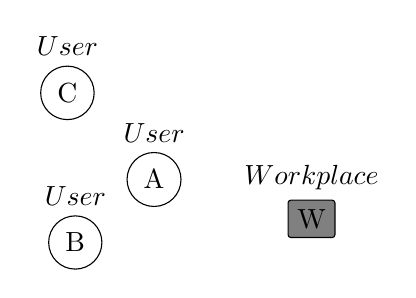
\begin{tikzpicture}
				\node[draw, circle, label=above:{$User$}] (A)at(-1.5, 0.5) {A};
				\node[draw, circle, label=above:{$User$}] (B)at(-2.5, -0.3) {B};
				\node[draw, circle, label=above:{$User$}] (C)at(-2.6, 1.6) {C};
				\node[draw, rectangle, rounded corners=1pt, fill=gray!100, label=above:{$Workplace$}] (W)at(0.5, 0) {W};
			\end{tikzpicture}
			\caption{User requests}
		\end{subfigure}%
		\begin{subfigure}{.5\textwidth}
			\centering
			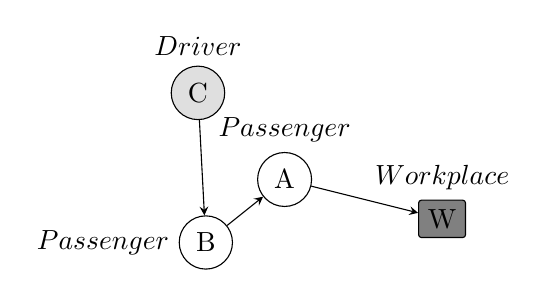
\begin{tikzpicture}
				\node[draw, circle, label=above:{$Passenger$}] (A)at(-1.5, 0.5) {A};
				\node[draw, circle, label=left:{$Passenger$}] (B)at(-2.5, -0.3) {B};
				\node[draw, circle, fill=gray!25, label=above:{$Driver$}] (C)at(-2.6, 1.6) {C};
				\node[draw, rectangle, rounded corners=1pt, fill=gray!100, label=above:{$Workplace$}] (W)at(0.5, 0) {W};
				\draw[->, >=stealth] (C) -- (B);
				\draw[->, >=stealth] (B) -- (A);
				\draw[->, >=stealth] (A) -- (W);
			\end{tikzpicture}
			\caption{A solution}
		\end{subfigure}
		\caption{Same workplace}
		\label{fig:same workplace}
	\end{figure}
	
	In Figure \ref{fig:same workplace}, we have an example of passengers who want to get to work. In addition, we want every user to go to their own workplace.
	
	\begin{figure}[H]
		\centering
		\begin{subfigure}{.5\textwidth}
			\centering
			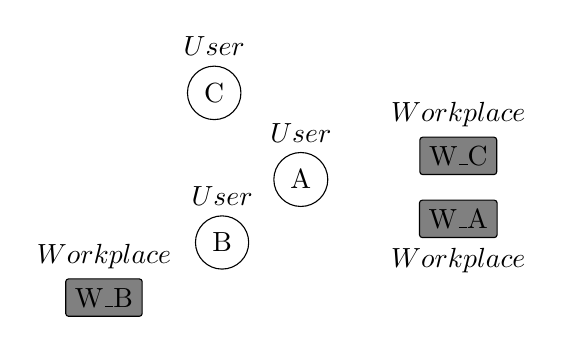
\begin{tikzpicture}
				\node[draw, circle, label=above:{$User$}] (A)at(-1.5, 0.5) {A};
				\node[draw, circle, label=above:{$User$}] (B)at(-2.5, -0.3) {B};
				\node[draw, circle, label=above:{$User$}] (C)at(-2.6, 1.6) {C};
				\node[draw, rectangle, rounded corners=1pt, fill=gray!100, label=below:{$Workplace$}] (WA)at(0.5, 0) {W\_A};
				\node[draw, rectangle, rounded corners=1pt, fill=gray!100, label=above:{$Workplace$}] (WC)at(0.5, 0.8) {W\_C};
				\node[draw, rectangle, rounded corners=1pt, fill=gray!100, label=above:{$Workplace$}] (WB)at(-4, -1) {W\_B};
			\end{tikzpicture}
			\caption{User requests}
		\end{subfigure}%
		\begin{subfigure}{.5\textwidth}
			\centering
			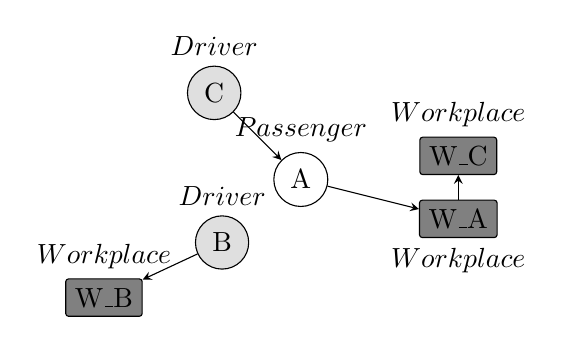
\begin{tikzpicture}
				\node[draw, circle, label=above:{$Passenger$}] (A)at(-1.5, 0.5) {A};
				\node[draw, circle, fill=gray!25, label=above:{$Driver$}] (B)at(-2.5, -0.3) {B};
				\node[draw, circle, fill=gray!25, label=above:{$Driver$}] (C)at(-2.6, 1.6) {C};
				\node[draw, rectangle, rounded corners=1pt, fill=gray!100, label=below:{$Workplace$}] (WA)at(0.5, 0) {W\_A};
				\node[draw, rectangle, rounded corners=1pt, fill=gray!100, label=above:{$Workplace$}] (WC)at(0.5, 0.8) {W\_C};
				\node[draw, rectangle, rounded corners=1pt, fill=gray!100, label=above:{$Workplace$}] (WB)at(-4, -1) {W\_B};
				\draw[->, >=stealth] (C) -- (A);
				\draw[->, >=stealth] (A) -- (WA);
				\draw[->, >=stealth] (WA) -- (WC);
				\draw[->, >=stealth] (B) -- (WB);
			\end{tikzpicture}
			\caption{A solution}
		\end{subfigure}
		\caption{Different workplaces}
		\label{fig:different workplaces}
	\end{figure}
	
	In Figure \ref{fig:different workplaces}, the user's work location $B$ is in the opposite direction to the user's work locations $A$ and $C$, the separation into two pools is evident. However, another parameter is added to the problem, the management of time windows.
	
	\begin{figure}[H]
		\centering
		\begin{subfigure}{.5\textwidth}
			\centering
			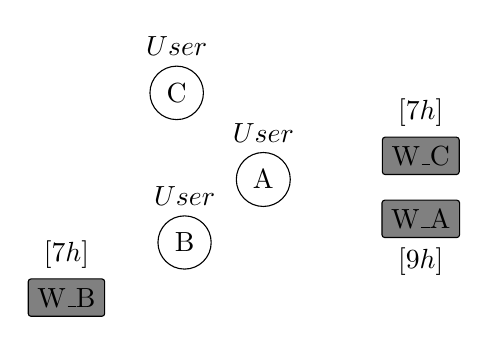
\begin{tikzpicture}
				\node[draw, circle, label=above:{$User$}] (A)at(-1.5, 0.5) {A};
				\node[draw, circle, label=above:{$User$}] (B)at(-2.5, -0.3) {B};
				\node[draw, circle, label=above:{$User$}] (C)at(-2.6, 1.6) {C};
				\node[draw, rectangle, rounded corners=1pt, fill=gray!100, label=below:{$[9h]$}] (WA)at(0.5, 0) {W\_A};
				\node[draw, rectangle, rounded corners=1pt, fill=gray!100, label=above:{$[7h]$}] (WC)at(0.5, 0.8) {W\_C};
				\node[draw, rectangle, rounded corners=1pt, fill=gray!100, label=above:{$[7h]$}] (WB)at(-4, -1) {W\_B};
			\end{tikzpicture}
			\caption{User requests}
		\end{subfigure}%
		\begin{subfigure}{.5\textwidth}
			\centering
			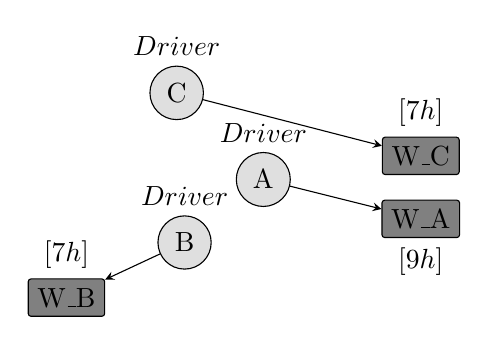
\begin{tikzpicture}
				\node[draw, circle, fill=gray!25, label=above:{$Driver$}] (A)at(-1.5, 0.5) {A};
				\node[draw, circle, fill=gray!25, label=above:{$Driver$}] (B)at(-2.5, -0.3) {B};
				\node[draw, circle, fill=gray!25, label=above:{$Driver$}] (C)at(-2.6, 1.6) {C};
				\node[draw, rectangle, rounded corners=1pt, fill=gray!100, label=below:{$[9h]$}] (WA)at(0.5, 0) {W\_A};
				\node[draw, rectangle, rounded corners=1pt, fill=gray!100, label=above:{$[7h]$}] (WC)at(0.5, 0.8) {W\_C};
				\node[draw, rectangle, rounded corners=1pt, fill=gray!100, label=above:{$[7h]$}] (WB)at(-4, -1) {W\_B};
				\draw[->, >=stealth] (C) -- (WC);
				\draw[->, >=stealth] (A) -- (WA);
				\draw[->, >=stealth] (B) -- (WB);
			\end{tikzpicture}
			\caption{A solution}
		\end{subfigure}
		\caption{Different time windows}
		\label{fig:different time windows}
	\end{figure}
	
	In Figure \ref{fig:different time windows}, each user has one hour of work at which he starts working. The user $A$'s work starts later than the user $C$'s work, which forces each user to take his car.
	
	\begin{figure}[H]
		\centering
		\begin{subfigure}{.5\textwidth}
			\centering
			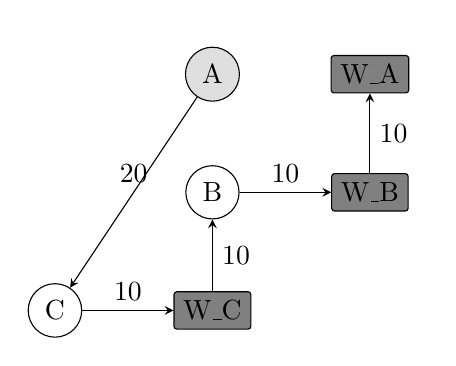
\begin{tikzpicture}
				\node[draw, circle, fill=gray!25, label=above:{$$}] (A)at(-1.5, 1) {A};
				\node[draw, circle, label=above:{$$}] (B)at(-1.5, -0.5) {B};
				\node[draw, circle, label=above:{$$}] (C)at(-3.5, -2) {C};
				\node[draw, rectangle, rounded corners=1pt, fill=gray!100, label=right:{$$}] (WA)at(0.5, 1) {W\_A};
				\node[draw, rectangle, rounded corners=1pt, fill=gray!100, label=right:{$$}] (WB)at(0.5, -0.5) {W\_B};
				\node[draw, rectangle, rounded corners=1pt, fill=gray!100, label=right:{$$}] (WC)at(-1.5, -2) {W\_C};
				\draw[->, >=stealth, above] (A) -- (C) node[midway] {$20$};
				\draw[->, >=stealth, above] (C) -- (WC) node[midway] {$10$};
				\draw[->, >=stealth, right] (WC) -- (B) node[midway] {$10$};
				\draw[->, >=stealth, above] (B) -- (WB) node[midway] {$10$};
				\draw[->, >=stealth, right] (WB) -- (WA) node[midway] {$10$};
			\end{tikzpicture}
			\caption{Total cost = 60}
		\end{subfigure}%
		\begin{subfigure}{.5\textwidth}
			\centering
			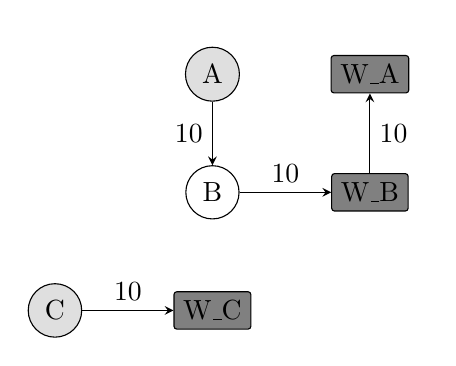
\begin{tikzpicture}
				\node[draw, circle, fill=gray!25, label=above:{$$}] (A)at(-1.5, 1) {A};
				\node[draw, circle, label=above:{$$}] (B)at(-1.5, -0.5) {B};
				\node[draw, circle, fill=gray!25, label=above:{$$}] (C)at(-3.5, -2) {C};
				\node[draw, rectangle, rounded corners=1pt, fill=gray!100, label=right:{$$}] (WA)at(0.5, 1) {W\_A};
				\node[draw, rectangle, rounded corners=1pt, fill=gray!100, label=right:{$$}] (WB)at(0.5, -0.5) {W\_B};
				\node[draw, rectangle, rounded corners=1pt, fill=gray!100, label=right:{$$}] (WC)at(-1.5, -2) {W\_C};
				\draw[->, >=stealth, left] (A) -- (B) node[midway] {$10$};
				\draw[->, >=stealth, above] (C) -- (WC) node[midway] {$10$};
				\draw[->, >=stealth, above] (B) -- (WB) node[midway] {$10$};
				\draw[->, >=stealth, right] (WB) -- (WA) node[midway] {$10$};
			\end{tikzpicture}
			\caption{Total cost = 40}
		\end{subfigure}
		\caption{Minimization of the costs}
		\label{fig:costs minimization}
	\end{figure}
	On each arc is represented a distance / cost of fuel to go from one peak to another. In the Figure \ref{fig:costs minimization}, the solution proposed in $(b)$ is more optimal than that proposed in $(a)$ for the same data set, since the total distance cost is lower.
	
	% Original characteristics
	\section{Original characteristics}
	\subsection*{Return management}
	
	Return management remains an original criterion in the DCPP because Mr. GUO uses it in the context of the LCPP \cite{guometaheuristics2012}, and the objective of the LCPP is to have stable pools, with the same people for the home-work trip and for the corresponding return trip. Although we do not have this constraint in the DCPP, we can have different pools.

	\begin{figure}[H]
		\centering
		\begin{subfigure}{.5\textwidth}
			\centering
			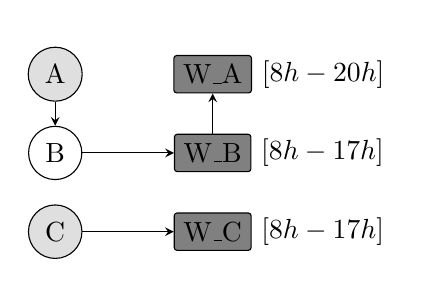
\begin{tikzpicture}
				\node[draw, circle, fill=gray!25, label=above:{$$}] (A)at(-1.5, 0.5) {A};
				\node[draw, circle, label=above:{$$}] (B)at(-1.5, -0.5) {B};
				\node[draw, circle, fill=gray!25, label=above:{$$}] (C)at(-1.5, -1.5) {C};
				\node[draw, rectangle, rounded corners=1pt, fill=gray!100, label=right:{$[8h-20h]$}] (WA)at(0.5, 0.5) {W\_A};
				\node[draw, rectangle, rounded corners=1pt, fill=gray!100, label=right:{$[8h-17h]$}] (WB)at(0.5, -0.5) {W\_B};
				\node[draw, rectangle, rounded corners=1pt, fill=gray!100, label=right:{$[8h-17h]$}] (WC)at(0.5, -1.5) {W\_C};
				\draw[->, >=stealth] (A) -- (B);
				\draw[->, >=stealth] (B) -- (WB);
				\draw[->, >=stealth] (WB) -- (WA);
				\draw[->, >=stealth] (C) -- (WC);
			\end{tikzpicture}
			\caption{Home-to-work trip}
		\end{subfigure}%
		\begin{subfigure}{.5\textwidth}
			\centering
			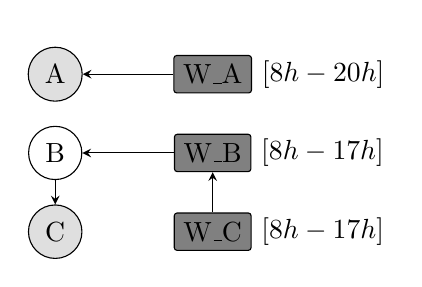
\begin{tikzpicture}
				\node[draw, circle, fill=gray!25, label=above:{$$}] (A)at(-1.5, 0.5) {A};
				\node[draw, circle, label=above:{$$}] (B)at(-1.5, -0.5) {B};
				\node[draw, circle, fill=gray!25, label=above:{$$}] (C)at(-1.5, -1.5) {C};
				\node[draw, rectangle, rounded corners=1pt, fill=gray!100, label=right:{$[8h-20h]$}] (WA)at(0.5, 0.5) {W\_A};
				\node[draw, rectangle, rounded corners=1pt, fill=gray!100, label=right:{$[8h-17h]$}] (WB)at(0.5, -0.5) {W\_B};
				\node[draw, rectangle, rounded corners=1pt, fill=gray!100, label=right:{$[8h-17h]$}] (WC)at(0.5, -1.5) {W\_C};
				\draw[->, >=stealth] (WA) -- (A);
				\draw[->, >=stealth] (WC) -- (WB);
				\draw[->, >=stealth] (WB) -- (B);
				\draw[->, >=stealth] (B) -- (C);
			\end{tikzpicture}
			\caption{Return trip}
		\end{subfigure}
		\caption{Return management}
		\label{fig:Return management}
	\end{figure}
	
	Figure \ref{fig:Return management} represents a home-work trip (a) and the corresponding return trip (b). We can see that the composition of the vehicles changes, the schedules allowing it.
	
	\subsection*{An user with multiple homes and workplaces}
	One of the other originalities of the basic problem is to have places of return from work different from those where we go to work. This is useful for example for someone who has a job where he has to change places during the day, or if someone wants to go to an activity after work. The purpose of this feature is to give more freedom to people who want to carpool.
	
	\begin{figure}[H]
		\centering
		\begin{subfigure}{.5\textwidth}
			\centering
			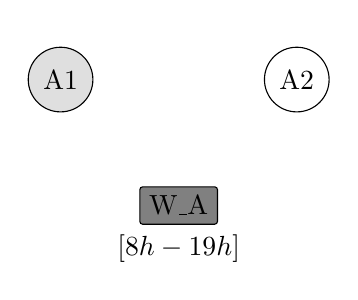
\begin{tikzpicture}
				\node[draw, circle, fill=gray!25, label=above:{$$}] (A1)at(-1.5, 1) {A1};
				\node[draw, circle, label=above:{$$}] (A2)at(1.5, 1) {A2};
				\node[draw, rectangle, rounded corners=1pt, fill=gray!100, label=below:{$[8h-19h]$}] (WA)at(0, -0.6) {W\_A};
			\end{tikzpicture}
			\caption{ Data }
		\end{subfigure}%
		\begin{subfigure}{.5\textwidth}
			\centering
			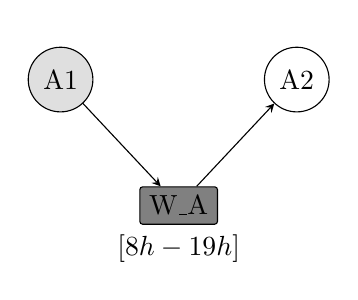
\begin{tikzpicture}
				\node[draw, circle, fill=gray!25, label=above:{$$}] (A1)at(-1.5, 1) {A1};
				\node[draw, circle, label=above:{$$}] (A2)at(1.5, 1) {A2};
				\node[draw, rectangle, rounded corners=1pt, fill=gray!100, label=below:{$[8h-19h]$}] (WA)at(0, -0.6) {W\_A};
				\draw[->, >=stealth, above] (A1) -- (WA) node[midway] {$$};
				\draw[->, >=stealth, above] (WA) -- (A2) node[midway] {$$};
			\end{tikzpicture}
			\caption{ Solution }
		\end{subfigure}
		\caption{Multiple homes}
		\label{fig:Several homes}
	\end{figure}
	
	In Figure \ref{fig:Several homes} we can see a way to materialize the different homes of the same person with $A1$ corresponding to the home address of departure, and $A2$ corresponding to the place of return $(a)$. The proposed solution path for this person going after work to his second home address is shown in $(b)$.
	
	\begin{figure}[H]
		\centering
		\begin{subfigure}{.5\textwidth}
			\centering
			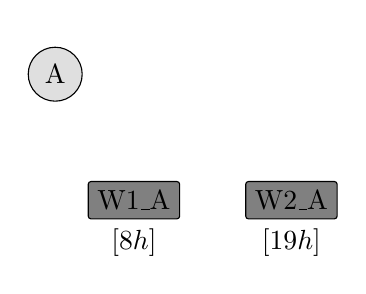
\begin{tikzpicture}
				\node[draw, circle, fill=gray!25, label=above:{$$}] (A)at(-1.5, 1) {A};
				\node[draw, rectangle, rounded corners=1pt, fill=gray!100, label=below:{$[8h]$}] (W1A)at(-0.5, -0.6) {W1\_A};
				\node[draw, rectangle, rounded corners=1pt, fill=gray!100, label=below:{$[19h]$}] (W2A)at(1.5, -0.6) {W2\_A};
			\end{tikzpicture}
			\caption{ Data }
		\end{subfigure}%
		\begin{subfigure}{.5\textwidth}
			\centering
			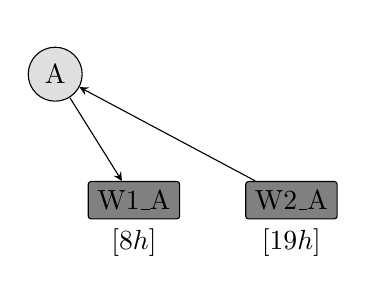
\begin{tikzpicture}
				\node[draw, circle, fill=gray!25, label=above:{$$}] (A)at(-1.5, 1) {A};
				\node[draw, rectangle, rounded corners=1pt, fill=gray!100, label=below:{$[8h]$}] (W1A)at(-0.5, -0.6) {W1\_A};
				\node[draw, rectangle, rounded corners=1pt, fill=gray!100, label=below:{$[19h]$}] (W2A)at(1.5, -0.6) {W2\_A};
				\draw[->, >=stealth, above] (A) -- (W1A) node[midway] {$$};
				\draw[->, >=stealth, above] (W2A) -- (A) node[midway] {$$};
			\end{tikzpicture}
			\caption{ Solution }
		\end{subfigure}
		\caption{Multiple workplaces}
		\label{fig:Several workplaces}
	\end{figure}
	
	Figure \ref{fig:Several workplaces} shows the notation used when a person has multiple workplaces (a) using the same numerical nomenclature, and the corresponding solution (b). Note that there is no arc between the two places of work because the path from one to the other is independent of our system.
	
	\begin{figure}[H]
		\centering
		\begin{subfigure}{.5\textwidth}
			\centering
			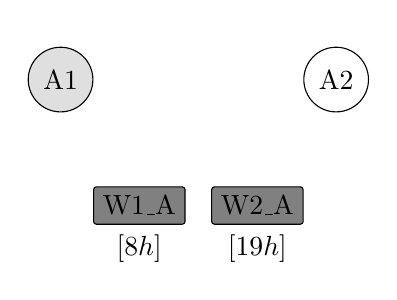
\begin{tikzpicture}
				\node[draw, circle, fill=gray!25, label=above:{$$}] (A1)at(-1.5, 1) {A1};
				\node[draw, circle, label=above:{$$}] (A2)at(2, 1) {A2};
				\node[draw, rectangle, rounded corners=1pt, fill=gray!100, label=below:{$[8h]$}] (W1A)at(-0.5, -0.6) {W1\_A};
				\node[draw, rectangle, rounded corners=1pt, fill=gray!100, label=below:{$[19h]$}] (W2A)at(1, -0.6) {W2\_A};
			\end{tikzpicture}
			\caption{ Data }
		\end{subfigure}%
		\begin{subfigure}{.5\textwidth}
			\centering
			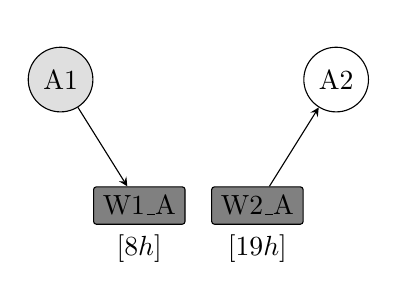
\begin{tikzpicture}
				\node[draw, circle, fill=gray!25, label=above:{$$}] (A1)at(-1.5, 1) {A1};
				\node[draw, circle, label=above:{$$}] (A2)at(2, 1) {A2};
				\node[draw, rectangle, rounded corners=1pt, fill=gray!100, label=below:{$[8h]$}] (W1A)at(-0.5, -0.6) {W1\_A};
				\node[draw, rectangle, rounded corners=1pt, fill=gray!100, label=below:{$[19h]$}] (W2A)at(1, -0.6) {W2\_A};
				\draw[->, >=stealth, above] (A1) -- (W1A) node[midway] {$$};
				\draw[->, >=stealth, above] (W2A) -- (A2) node[midway] {$$};
			\end{tikzpicture}
			\caption{ Solution }
		\end{subfigure}
		\caption{Multiple homes and workplaces}
		\label{fig:Several homes and workplaces}
	\end{figure}
	
	Figure \ref{fig:Several homes and workplaces} represents the union of the two previous examples. The user makes the $A1-W1_A$ trip in the morning, then makes the $W2_A-A2$ trip in the evening.
	
	\subsection{CPP class}
	
	Carpooling is studied since the seventies \cite{wohlmethodology1970} \cite{sagnerimpact1974}, and two types of carpooling problems have been defined since the 2000s \cite{kotharigenghis-multiagent2004} \cite{maniezzoants2004} \cite{calvodistributed2004}. There are significant differences depending on the literature chosen regarding the definition of these two groups.\newline
		\tab The Daily CarPooling Problem \textbf{DCPP} concerns the formation of pools, possibly different each day. We can say that the pools of each day are independent of the elders.\newline
		\tab The Long Term CarPooling Problem \textbf{LCPP} concerns the formation of regular and stable pools over a given period. Some articles talk about the variation of who takes his car in each pool formed \cite{guometaheuristics2012}. 
	
	\subsection*{Difference between DCPP and LCPP}
	Each Figure below represents (a) the requests and (b) a proposed solution. Each circle represents a request from a user wishing to go to work. The work is represented by a dark grey square. \newline
	In the solution, users who take their car, thus becoming drivers, are represented by a light grey circle. The arches represent the path taken by the driver.\newline 
	The following Figures show examples to highlight the difference between the DCPP and the LCPP over \textbf{two consecutive days}.
	
	\begin{figure}[H]
		\centering
		\begin{subfigure}{.5\textwidth}
			\centering
			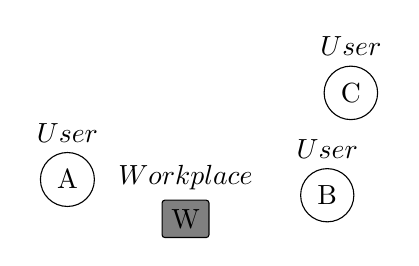
\begin{tikzpicture}
				\node[draw, circle, label=above:{$User$}] (A)at(-1, 0.5) {A};
				\node[draw, circle, label=above:{$User$}] (B)at(2.3, 0.3) {B};
				\node[draw, circle, label=above:{$User$}] (C)at(2.6, 1.6) {C};
				\node[draw, rectangle, rounded corners=1pt, fill=gray!100, label=above:{$Workplace$}] (W)at(0.5, 0) {W};
			\end{tikzpicture}
			\caption{User Requests}
		\end{subfigure}%
		\begin{subfigure}{.5\textwidth}
			\centering
			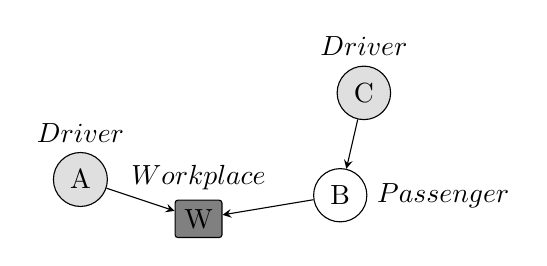
\begin{tikzpicture}
				\node[draw, circle, fill=gray!25, label=above:{$Driver$}] (A)at(-1, 0.5) {A};
				\node[draw, circle, label=right:{$Passenger$}] (B)at(2.3, 0.3) {B};
				\node[draw, circle, fill=gray!25, label=above:{$Driver$}] (C)at(2.6, 1.6) {C};
				\node[draw, rectangle, rounded corners=1pt, fill=gray!100, label=above:{$Workplace$}] (W)at(0.5, 0) {W};
				\draw[->, >=stealth] (C) -- (B);
				\draw[->, >=stealth] (B) -- (W);
				\draw[->, >=stealth] (A) -- (W);
			\end{tikzpicture}
			\caption{A solution}
		\end{subfigure}
		\caption{DCPP: First day}
		\label{fig:DCPP D1}
	\end{figure}
	
	Figure \ref{fig:DCPP D1} shows a possible instance of the DCPP, with a set of requests and a solution.

	\begin{figure}[H]
		\centering
		\begin{subfigure}{.5\textwidth}
			\centering
			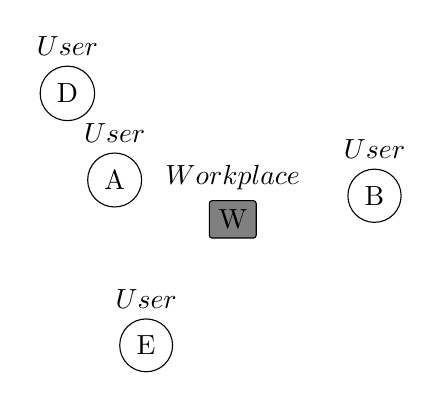
\begin{tikzpicture}
				\node[draw, circle, label=above:{$User$}] (A)at(-1, 0.5) {A};
				\node[draw, circle, label=above:{$User$}] (B)at(2.3, 0.3) {B};
				\node[draw, circle, label=above:{$User$}] (D)at(-1.6, 1.6) {D};
				\node[draw, circle, label=above:{$User$}] (E)at(-0.6, -1.6) {E};
				\node[draw, rectangle, rounded corners=1pt, fill=gray!100, label=above:{$Workplace$}] (W)at(0.5, 0) {W};
		\end{tikzpicture}
		\caption{User Requests}
		\end{subfigure}%
		\begin{subfigure}{.5\textwidth}
			\centering
			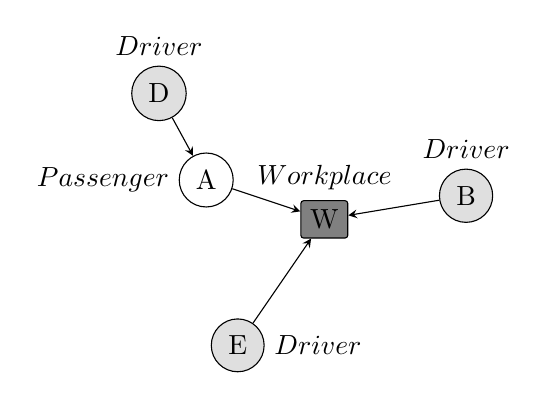
\begin{tikzpicture}
				\node[draw, circle, label=left:{$Passenger$}] (A)at(-1, 0.5) {A};
				\node[draw, circle, fill=gray!25, label=above:{$Driver$}] (B)at(2.3, 0.3) {B};
				\node[draw, circle, fill=gray!25, label=above:{$Driver$}] (D)at(-1.6, 1.6) {D};
				\node[draw, circle, fill=gray!25, label=right:{$Driver$}] (E)at(-0.6, -1.6) {E};
				\node[draw, rectangle, rounded corners=1pt, fill=gray!100, label=above:{$Workplace$}] (W)at(0.5, 0) {W};
				\draw[->, >=stealth] (D) -- (A);
				\draw[->, >=stealth] (A) -- (W);
				\draw[->, >=stealth] (B) -- (W);
				\draw[->, >=stealth] (E) -- (W);
			\end{tikzpicture}
			\caption{A solution}
		\end{subfigure}
		\caption{DCPP: Second day}
		\label{fig:DCPP D2}
	\end{figure}
	
	Figure \ref{fig:DCPP D2} represents the following day of the Figure \ref{fig:DCPP D1}. We can see that there are no longer the same users. Some have not renewed their requests, and some new requests must be taken into account. Thus, we can see that the user $A$ becomes a passenger on the second day, whereas he left to work alone on the first day. The user $B$ was a passenger on the first day, and goes to work alone on the second day.
	\newpar
	Now let's see the LCPP examples.
	
	\begin{figure}[H]
		\centering
		\begin{subfigure}{.5\textwidth}
			\centering
			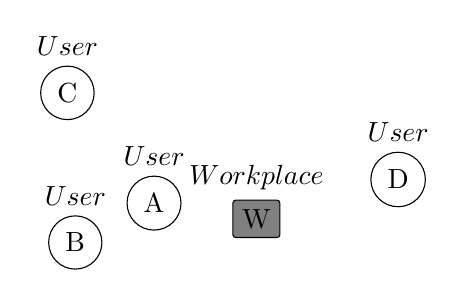
\begin{tikzpicture}
				\node[draw, circle, label=above:{$User$}] (A)at(-1.5, 0.2) {A};
				\node[draw, circle, label=above:{$User$}] (B)at(-2.5, -0.3) {B};
				\node[draw, circle, label=above:{$User$}] (C)at(-2.6, 1.6) {C};
				\node[draw, circle, label=above:{$User$}] (D)at(1.6, 0.5) {D};
				\node[draw, rectangle, rounded corners=1pt, fill=gray!100, label=above:{$Workplace$}] (W)at(-0.2, 0) {W};
			\end{tikzpicture}
			\caption{User Requests}
		\end{subfigure}%
		\begin{subfigure}{.5\textwidth}
			\centering
			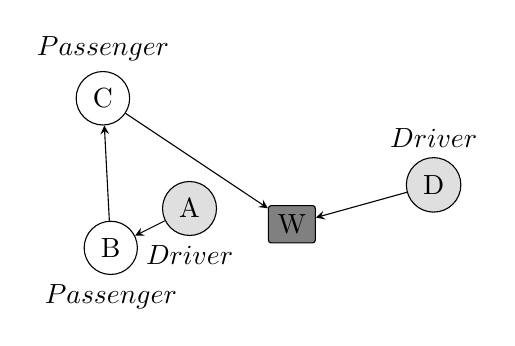
\begin{tikzpicture}
				\node[draw, circle, fill=gray!25, label=below:{$Driver$}] (A)at(-1.5, 0.2) {A};
				\node[draw, circle, label=below:{$Passenger$}] (B)at(-2.5, -0.3) {B};
				\node[draw, circle, label=above:{$Passenger$}] (C)at(-2.6, 1.6) {C};
				\node[draw, circle, fill=gray!25, label=above:{$Driver$}] (D)at(1.6, 0.5) {D};
				\node[draw, rectangle, rounded corners=1pt, fill=gray!100, label=above:{$$}] (W)at(-0.2, 0) {W};
				\draw[->, >=stealth] (A) -- (B);
				\draw[->, >=stealth] (B) -- (C);
				\draw[->, >=stealth] (C) -- (W);
				\draw[->, >=stealth] (D) -- (W);
			\end{tikzpicture} 
			\caption{A solution}
		\end{subfigure}
		\caption{LCPP: First day}
		\label{fig:LCPP D1}
	\end{figure}
	
	Figure \ref{fig:LCPP D1} concerns the LCPP, with the same pattern as in Figure \ref{fig:DCPP D2}.
	
	\begin{figure}[H]
		\centering
		\begin{subfigure}{.5\textwidth}
			\centering
			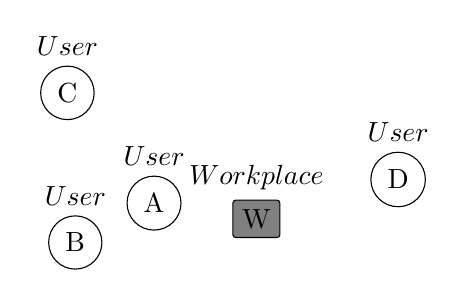
\begin{tikzpicture}
				\node[draw, circle, label=above:{$User$}] (A)at(-1.5, 0.2) {A};
				\node[draw, circle, label=above:{$User$}] (B)at(-2.5, -0.3) {B};
				\node[draw, circle, label=above:{$User$}] (C)at(-2.6, 1.6) {C};
				\node[draw, circle, label=above:{$User$}] (D)at(1.6, 0.5) {D};
				\node[draw, rectangle, rounded corners=1pt, fill=gray!100, label=above:{$Workplace$}] (W)at(-0.2, 0) {W};
			\end{tikzpicture}
			\caption{User Requests}
		\end{subfigure}%
		\begin{subfigure}{.5\textwidth}
			\centering
			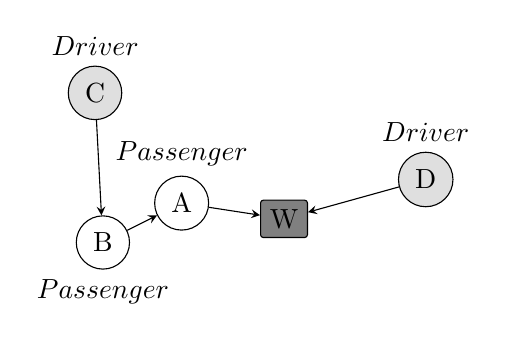
\begin{tikzpicture}
				\node[draw, circle, label=above:{$Passenger$}] (A)at(-1.5, 0.2) {A};
				\node[draw, circle, label=below:{$Passenger$}] (B)at(-2.5, -0.3) {B};
				\node[draw, circle, fill=gray!25, label=above:{$Driver$}] (C)at(-2.6, 1.6) {C};
				\node[draw, circle, fill=gray!25, label=above:{$Driver$}] (D)at(1.6, 0.5) {D};
				\node[draw, rectangle, rounded corners=1pt, fill=gray!100, label=above:{$$}] (W)at(-0.2, 0) {W};
				\draw[->, >=stealth] (C) -- (B);
				\draw[->, >=stealth] (B) -- (A);
				\draw[->, >=stealth] (A) -- (W);
				\draw[->, >=stealth] (D) -- (W);
			\end{tikzpicture}
			\caption{A solution}
		\end{subfigure}
		\caption{LCPP: Second day}
		\label{fig:LCPP D2}
	\end{figure}
	
	In Figure \ref{fig:LCPP D2}, the regularity is put forward: we have the same users as in Figure \ref{fig:LCPP D1}. The pools have remained, the solution is to vary the drivers. Changes may obviously occur, however the goal remains to maintain a certain consistency.
	\newpar
	Now that we know what carpooling is, we will see what are the issues of carpooling. 

	\subsection*{Another kind of time windows}
	
	Another originality is the way we manage time windows. Indeed, it corresponds to an authorized advance time before the beginning of the work. The same thing on the way home, with an authorized waiting time at work after the end of work. \newline
	We have time windows where the user must leave home in this interval: \newline
	{[work start time + maximum travel time, work start time + direct travel time]} \newline
	and time of arrival at work in that interval: \newline
	{work start time - time allocated in advance, work start time]}.
	
	\begin{figure}[H]
		\centering
		\begin{subfigure}{.5\textwidth}
			\centering
			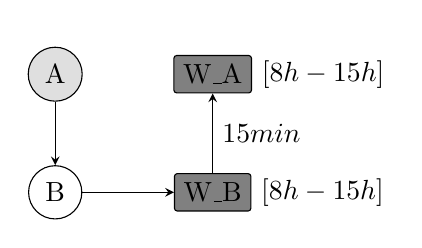
\begin{tikzpicture}
				\node[draw, circle, fill=gray!25, label=above:{$$}] (A)at(-1.5, 1) {A};
				\node[draw, circle, label=above:{$$}] (B)at(-1.5, -0.5) {B};
				\node[draw, rectangle, rounded corners=1pt, fill=gray!100, label=right:{$[8h-15h]$}] (WA)at(0.5, 1) {W\_A};
				\node[draw, rectangle, rounded corners=1pt, fill=gray!100, label=right:{$[8h-15h]$}] (WB)at(0.5, -0.5) {W\_B};
				\draw[->, >=stealth, above] (A) -- (B) node[midway] {$$};
				\draw[->, >=stealth, above] (B) -- (WB) node[midway] {$$};
				\draw[->, >=stealth, right] (WB) -- (WA) node[midway] {$15min$};
			\end{tikzpicture}
			\caption{Allowed advance waiting time = 20 min }
		\end{subfigure}%
		\begin{subfigure}{.5\textwidth}
			\centering
			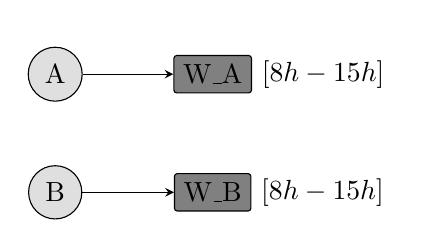
\begin{tikzpicture}
				\node[draw, circle, fill=gray!25, label=above:{$$}] (A)at(-1.5, 1) {A};
				\node[draw, circle, fill=gray!25, label=above:{$$}] (B)at(-1.5, -0.5) {B};
				\node[draw, rectangle, rounded corners=1pt, fill=gray!100, label=right:{$[8h-15h]$}] (WA)at(0.5, 1) {W\_A};
				\node[draw, rectangle, rounded corners=1pt, fill=gray!100, label=right:{$[8h-15h]$}] (WB)at(0.5, -0.5) {W\_B};
				\draw[->, >=stealth, above] (A) -- (WA) node[midway] {$$};
				\draw[->, >=stealth, above] (B) -- (WB) node[midway] {$$};
			\end{tikzpicture}
			\caption{Allowed advance waiting time = 10 min }
		\end{subfigure}
		\caption{Arrival to work waiting time}
		\label{fig:Arrival to work waiting time}
	\end{figure}
	
	In Figure \ref{fig:Arrival to work waiting time} we can see that it takes 15 minutes to travel between the two workplaces. If it is allowed to have an advance waiting time of 20 minutes (a), then a user can drop the other one 15 minutes in advance, and has time to get to work on time. If, on the other hand, there is only 10 minutes of waiting time allowed, the solution is that everyone takes his car, so that there is no user too early.
	
	\begin{figure}[H]
		\centering
		\begin{subfigure}{.5\textwidth}
			\centering
			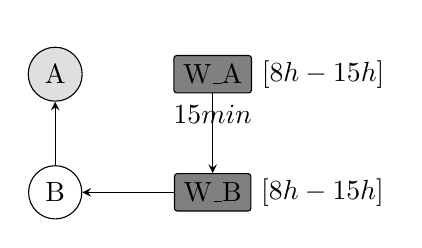
\begin{tikzpicture}
				\node[draw, circle, fill=gray!25, label=above:{$$}] (A)at(-1.5, 1) {A};
				\node[draw, circle, label=above:{$$}] (B)at(-1.5, -0.5) {B};
				\node[draw, rectangle, rounded corners=1pt, fill=gray!100, label=right:{$[8h-15h]$}] (WA)at(0.5, 1) {W\_A};
				\node[draw, rectangle, rounded corners=1pt, fill=gray!100, label=right:{$[8h-15h]$}] (WB)at(0.5, -0.5) {W\_B};
				\draw[->, >=stealth, above] (WA) -- (WB) node[midway] {$15min$};
				\draw[->, >=stealth, above] (WB) -- (B) node[midway] {$$};
				\draw[->, >=stealth, right] (B) -- (A) node[midway] {$$};
			\end{tikzpicture}
			\caption{Allowed waiting time after finishing work= 20 min }
		\end{subfigure}%
		\begin{subfigure}{.5\textwidth}
			\centering
			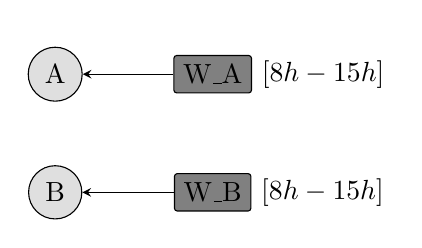
\begin{tikzpicture}
				\node[draw, circle, fill=gray!25, label=above:{$$}] (A)at(-1.5, 1) {A};
				\node[draw, circle, fill=gray!25, label=above:{$$}] (B)at(-1.5, -0.5) {B};
				\node[draw, rectangle, rounded corners=1pt, fill=gray!100, label=right:{$[8h-15h]$}] (WA)at(0.5, 1) {W\_A};
				\node[draw, rectangle, rounded corners=1pt, fill=gray!100, label=right:{$[8h-15h]$}] (WB)at(0.5, -0.5) {W\_B};
				\draw[->, >=stealth, above] (WA) -- (A) node[midway] {$$};
				\draw[->, >=stealth, above] (WB) -- (B) node[midway] {$$};
			\end{tikzpicture}
			\caption{Allowed waiting time after finishing work = 10 min }
		\end{subfigure}
		\caption{Departure from work waiting time}
		\label{fig:Departure from work waiting time}
	\end{figure}
	
	Figure \ref{fig:Departure from work waiting time} shows this time the return from work. This follows the same pattern as Figure \ref{fig:Arrival to work waiting time}, by allowing more or less waiting time after work, the solution can also evolve.

	\subsection*{Use of satellites places}
	
	Satellite locations are places where people can be dropped off and picked up, close to a place such as home or workplace. This can be useful to the problem, in order to have more similar data and perhaps to leave more possibilities of results. For example a motorway exit close to many workplaces within 1km walk can be a good satellite point.
	
	\begin{figure}[H]
		\centering
		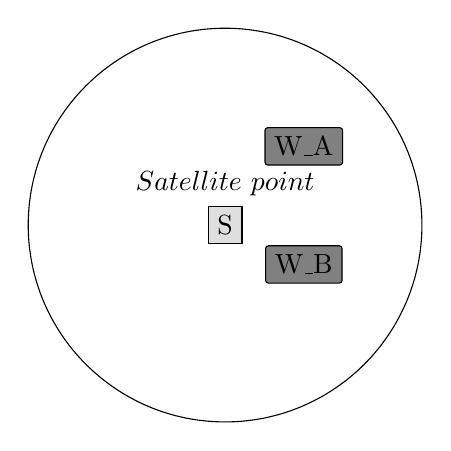
\begin{tikzpicture}
			\draw (0, 0) circle (2.5) ;
			\node[draw, rectangle, fill=gray!25, label=above:{$Satellite$ $point$}] (S)at(0, 0) {S};
			\node[draw, rectangle, rounded corners=1pt, fill=gray!100, label=right:{$$}] (WA)at(1, 1) {W\_A};
			\node[draw, rectangle, rounded corners=1pt, fill=gray!100, label=right:{$$}] (WB)at(1, -0.5) {W\_B};
		\end{tikzpicture}
		\caption{Satellite range}
		\label{fig:Satellite range}
	\end{figure}
	
	In Figure \ref{fig:Satellite range} we can observe a satellite point that can be used as the same point instead of using both workplaces.
	\newpar
	We will now see in which complexity class we can put this problem.

	%%%%%%%%%%%%%%%% COMPLEXITY %%%%%%%%%%%%%%%%%%%%
	\section{Complexity of the problem}
	
	To prove the complexity of the problem, we will take another problem whose complexity is known, and then prove that our problem is at least as difficult.
	
	\subsection{Hamiltonian Path Problem}

	A Hamiltonian path is a path that visits each vertex of the graph exactly once.\newline
	Let's consider a generic Hamiltonian Path Problem \textbf{HPP}: \newline
	\tab Let a graph $G=(V, E)$, with weighted edges $w:E\mapsto \mathbb{R}$, and a bound B.\newline
	Is there a Hamiltonian path in $G$ whose sum of weights is less or equal than $B$ ?\newline
	This problem is known to be of \textbf{NP-hard} complexity.
	
	\begin{figure}[H]
		\centering
		\begin{subfigure}{.5\textwidth}
			\centering
			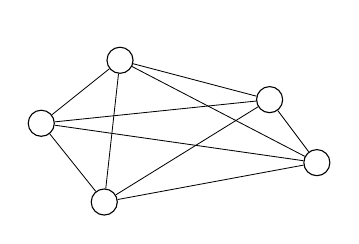
\begin{tikzpicture}
				\node[draw, circle, label=above:{$$}] (A)at(-1.2, -0.5) {};
				\node[draw, circle, label=above:{$$}] (B)at(-2, 0.5) {};
				\node[draw, circle, label=above:{$$}] (C)at(-1, 1.3) {};
				\node[draw, circle, label=above:{$$}] (D)at(0.9, 0.8) {};
				\node[draw, circle, label=above:{$$}] (E)at(1.5, 0) {};
				\draw[line width=0.3pt] (A) -- (B) node[midway] {$$};
				\draw[line width=0.3pt] (A) -- (C) node[midway] {$$};
				\draw[line width=0.3pt] (A) -- (D) node[midway] {$$};
				\draw[line width=0.3pt] (A) -- (E) node[midway] {$$};
				\draw[line width=0.3pt] (B) -- (C) node[midway] {$$};
				\draw[line width=0.3pt] (B) -- (D) node[midway] {$$};
				\draw[line width=0.3pt] (B) -- (E) node[midway] {$$};
				\draw[line width=0.3pt] (C) -- (D) node[midway] {$$};
				\draw[line width=0.3pt] (C) -- (E) node[midway] {$$};
				\draw[line width=0.3pt] (D) -- (E) node[midway] {$$};
			\end{tikzpicture}
			\caption{A complete graph}
		\end{subfigure}%
		\begin{subfigure}{.5\textwidth}
			\centering
			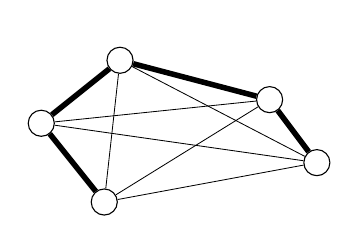
\begin{tikzpicture}
				\node[draw, circle, label=above:{$$}] (A)at(-1.2, -0.5) {};
				\node[draw, circle, label=above:{$$}] (B)at(-2, 0.5) {};
				\node[draw, circle, label=above:{$$}] (C)at(-1, 1.3) {};
				\node[draw, circle, label=above:{$$}] (D)at(0.9, 0.8) {};
				\node[draw, circle, label=above:{$$}] (E)at(1.5, 0) {};
				\draw[line width=2pt] (A) -- (B) node[midway] {$$};
				\draw[line width=0.3pt] (A) -- (C) node[midway] {$$};
				\draw[line width=0.3pt] (A) -- (D) node[midway] {$$};
				\draw[line width=0.3pt] (A) -- (E) node[midway] {$$};
				\draw[line width=2pt] (B) -- (C) node[midway] {$$};
				\draw[line width=0.3pt] (B) -- (D) node[midway] {$$};
				\draw[line width=0.3pt] (B) -- (E) node[midway] {$$};
				\draw[line width=2pt] (C) -- (D) node[midway] {$$};
				\draw[line width=0.3pt] (C) -- (E) node[midway] {$$};
				\draw[line width=2pt] (D) -- (E) node[midway] {$$};
			\end{tikzpicture}
			\caption{A corresponding Hamiltonian path solution}
		\end{subfigure}
		\caption{Example of a Hamiltonian path in a graph}
		\label{fig:Example of a Hamiltonian path in a graph}
	\end{figure}
	
	\noindent Figure \ref{fig:Example of a Hamiltonian path in a graph} represents an example of the Hamiltonian Path Problem.
	\newpar
	Now that we have defined the NP-hard problem, let's define our carpooling problem.
	
	\subsection{CarPooling Problem}
	
	Let's consider the following generic CarPooling Problem \textbf{CPP}: \newline
	\tab Users of a carpooling system issue requests of the form $(O_i, D_i)$ corresponding to the origin and destination of the user $i$. Each user can be either passenger or driver. \newline
	The origins and destinations correspond to the vertices of a graph.\newline
	\tab Consider a graph $G'=(V', E')$, where $V'$ is the union between the vertices origins and the vertices destination $V'=(O\cup D)$, and $E'$ corresponds to the edges between these vertices. \newline
	\tab Each of the origin vertices has a weight corresponding to a vehicle capacity $c:O\mapsto \mathbb{N}$. \newline
	\tab Each edge has a weight corresponding to a distance between the two vertices it relies $w':E\mapsto \mathbb{R}$.\newline
	The goal is to minimize the sum of distances so that each user goes from his origin to his destination.
	
	\begin{figure}[H]
		\centering
		\begin{subfigure}{.5\textwidth}
			\centering
			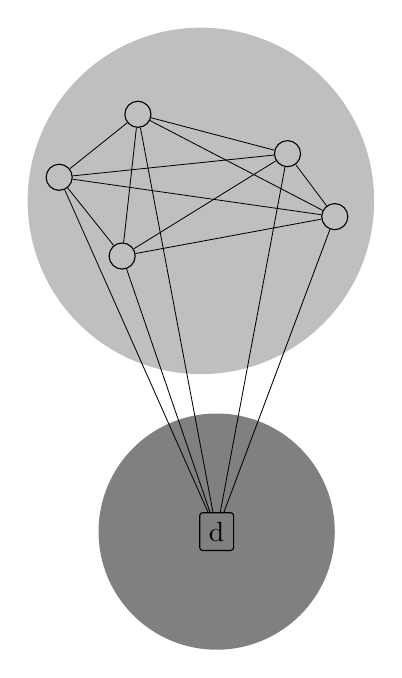
\begin{tikzpicture}
				\coordinate (O) at (-0.2, 0.2);
				\coordinate (DEST) at (0, -4);
				\fill[lightgray] (O) circle(2.2);
				\fill[gray] (DEST) circle(1.5);
				\node[draw, circle, label=above:{$$}] (A)at(-1.2, -0.5) {};
				\node[draw, circle, label=above:{$$}] (B)at(-2, 0.5) {};
				\node[draw, circle, label=above:{$$}] (C)at(-1, 1.3) {};
				\node[draw, circle, label=above:{$$}] (D)at(0.9, 0.8) {};
				\node[draw, circle, label=above:{$$}] (E)at(1.5, 0) {};
				\node[draw, rectangle, rounded corners=1pt, fill=gray!100, label=above:{$$}] (W)at(0, -4) {d};
				\draw[line width=0.3pt] (A) -- (B) node[midway] {$$};
				\draw[line width=0.3pt] (A) -- (C) node[midway] {$$};
				\draw[line width=0.3pt] (A) -- (D) node[midway] {$$};
				\draw[line width=0.3pt] (A) -- (E) node[midway] {$$};
				\draw[line width=0.3pt] (B) -- (C) node[midway] {$$};
				\draw[line width=0.3pt] (B) -- (D) node[midway] {$$};
				\draw[line width=0.3pt] (B) -- (E) node[midway] {$$};
				\draw[line width=0.3pt] (C) -- (D) node[midway] {$$};
				\draw[line width=0.3pt] (C) -- (E) node[midway] {$$};
				\draw[line width=0.3pt] (D) -- (E) node[midway] {$$};
				\draw[line width=0.3pt] (W) -- (A) node[midway] {$$};
				\draw[line width=0.3pt] (W) -- (B) node[midway] {$$};
				\draw[line width=0.3pt] (W) -- (C) node[midway] {$$};
				\draw[line width=0.3pt] (W) -- (D) node[midway] {$$};
				\draw[line width=0.3pt] (W) -- (E) node[midway] {$$};
			\end{tikzpicture}
			\caption{A complete graph}
		\end{subfigure}%
		\begin{subfigure}{.5\textwidth}
			\centering
			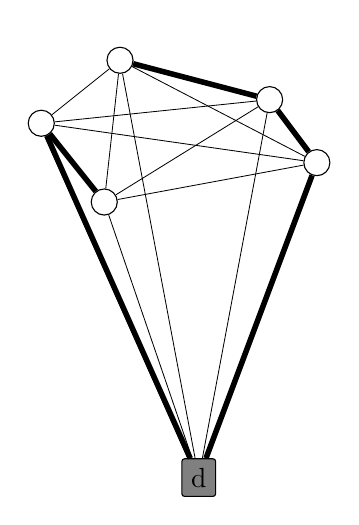
\begin{tikzpicture}
				\node[draw, circle, label=above:{$$}] (A)at(-1.2, -0.5) {};
				\node[draw, circle, label=above:{$$}] (B)at(-2, 0.5) {};
				\node[draw, circle, label=above:{$$}] (C)at(-1, 1.3) {};
				\node[draw, circle, label=above:{$$}] (D)at(0.9, 0.8) {};
				\node[draw, circle, label=above:{$$}] (E)at(1.5, 0) {};
				\node[draw, rectangle, rounded corners=1pt, fill=gray!100, label=above:{$$}] (W)at(0, -4) {d};
				\draw[line width=2pt] (A) -- (B) node[midway] {$$};
				\draw[line width=0.3pt] (A) -- (C) node[midway] {$$};
				\draw[line width=0.3pt] (A) -- (D) node[midway] {$$};
				\draw[line width=0.3pt] (A) -- (E) node[midway] {$$};
				\draw[line width=0.3pt] (B) -- (C) node[midway] {$$};
				\draw[line width=0.3pt] (B) -- (D) node[midway] {$$};
				\draw[line width=0.3pt] (B) -- (E) node[midway] {$$};
				\draw[line width=2pt] (C) -- (D) node[midway] {$$};
				\draw[line width=0.3pt] (C) -- (E) node[midway] {$$};
				\draw[line width=2pt] (D) -- (E) node[midway] {$$};
				\draw[line width=0.3pt] (W) -- (A) node[midway] {$$};
				\draw[line width=2pt] (W) -- (B) node[midway] {$$};
				\draw[line width=0.3pt] (W) -- (C) node[midway] {$$};
				\draw[line width=0.3pt] (W) -- (D) node[midway] {$$};
				\draw[line width=2pt] (W) -- (E) node[midway] {$$};
			\end{tikzpicture}
			\caption{A corresponding CarPooling solution}
		\end{subfigure}
		\caption{Example of the CarPooling problem}
		\label{fig:Example of the CarPooling problem}
	\end{figure}
	
	\noindent In Figure \ref{fig:Example of the CarPooling problem} $(a)$ we can see two areas: \newline
	\tab The lightgrayed zone corresponds to all the origins of the CPP.\newline
	\tab The grayed zone corresponds to all the destinations of the CPP, for more simplicity, we gather all the destinations at one point $d$.
	\newpar
	Let's understand the correspondences between the two problems.
	
	\subsection{Correspondences between the problems}
	
	In both cases, we are in complete charts. The graph follows the triangular inequality, the weight being related to the distance in the graph. \newline
	For any instance \textbf{I} of the HPP, there is an instance correspondence \textbf{I'} of the CPP.
	
	\begin{figure}[H]
		\centering
		\begin{subfigure}{.5\textwidth}
			\centering
			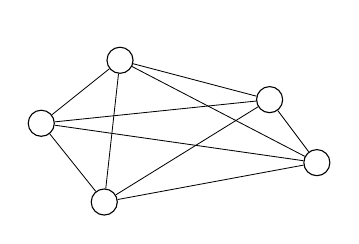
\begin{tikzpicture}
				\node[draw, circle, label=above:{$$}] (A)at(-1.2, -0.5) {};
				\node[draw, circle, label=above:{$$}] (B)at(-2, 0.5) {};
				\node[draw, circle, label=above:{$$}] (C)at(-1, 1.3) {};
				\node[draw, circle, label=above:{$$}] (D)at(0.9, 0.8) {};
				\node[draw, circle, label=above:{$$}] (E)at(1.5, 0) {};
				\draw[line width=0.3pt] (A) -- (B) node[midway] {$$};
				\draw[line width=0.3pt] (A) -- (C) node[midway] {$$};
				\draw[line width=0.3pt] (A) -- (D) node[midway] {$$};
				\draw[line width=0.3pt] (A) -- (E) node[midway] {$$};
				\draw[line width=0.3pt] (B) -- (C) node[midway] {$$};
				\draw[line width=0.3pt] (B) -- (D) node[midway] {$$};
				\draw[line width=0.3pt] (B) -- (E) node[midway] {$$};
				\draw[line width=0.3pt] (C) -- (D) node[midway] {$$};
				\draw[line width=0.3pt] (C) -- (E) node[midway] {$$};
				\draw[line width=0.3pt] (D) -- (E) node[midway] {$$};
			\end{tikzpicture}
			\caption{An instance I of the HPP}
		\end{subfigure}%
		\begin{subfigure}{.5\textwidth}
			\centering
			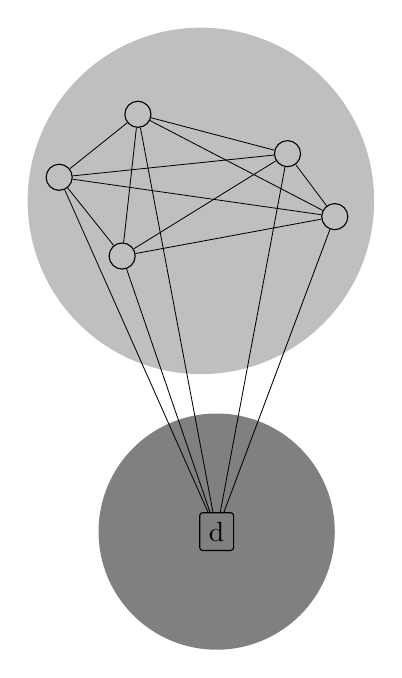
\begin{tikzpicture}
				\coordinate (O) at (-0.2, 0.2);
				\coordinate (DEST) at (0, -4);
				\fill[lightgray] (O) circle(2.2);
				\fill[gray] (DEST) circle(1.5);
				\node[draw, circle, label=above:{$$}] (A)at(-1.2, -0.5) {};
				\node[draw, circle, label=above:{$$}] (B)at(-2, 0.5) {};
				\node[draw, circle, label=above:{$$}] (C)at(-1, 1.3) {};
				\node[draw, circle, label=above:{$$}] (D)at(0.9, 0.8) {};
				\node[draw, circle, label=above:{$$}] (E)at(1.5, 0) {};
				\node[draw, rectangle, rounded corners=1pt, fill=gray!100, label=above:{$$}] (W)at(0, -4) {d};
				\draw[line width=0.3pt] (A) -- (B) node[midway] {$$};
				\draw[line width=0.3pt] (A) -- (C) node[midway] {$$};
				\draw[line width=0.3pt] (A) -- (D) node[midway] {$$};
				\draw[line width=0.3pt] (A) -- (E) node[midway] {$$};
				\draw[line width=0.3pt] (B) -- (C) node[midway] {$$};
				\draw[line width=0.3pt] (B) -- (D) node[midway] {$$};
				\draw[line width=0.3pt] (B) -- (E) node[midway] {$$};
				\draw[line width=0.3pt] (C) -- (D) node[midway] {$$};
				\draw[line width=0.3pt] (C) -- (E) node[midway] {$$};
				\draw[line width=0.3pt] (D) -- (E) node[midway] {$$};
				\draw[line width=0.3pt] (W) -- (A) node[midway] {$$};
				\draw[line width=0.3pt] (W) -- (B) node[midway] {$$};
				\draw[line width=0.3pt] (W) -- (C) node[midway] {$$};
				\draw[line width=0.3pt] (W) -- (D) node[midway] {$$};
				\draw[line width=0.3pt] (W) -- (E) node[midway] {$$};
			\end{tikzpicture}
			\caption{An corresponding instance I' of the CPP}
		\end{subfigure}
		\caption{An example of correspondences between a HPP and a CPP}
		\label{fig:Correspondences between a HPP and a CPP}
	\end{figure}
	
	\noindent As we can see in the Figure \ref{fig:Correspondences between a HPP and a CPP} each vertex of instance \textbf{I} corresponds to a vertex in the set origin of instance \textbf{I'}. \newline
	For each possible instance of the HPP we have for the CPP: \newline
	\tab $O=G$\newline
	\tab $D=\{d\}$\newline
	\tab $c_v=n=|V| \tab \forall v\in O$ \newline
	\tab $w_{ij}=w'_{ij} \tab \forall i, j\in V$\newline
	\tab $w_{vd}= W \tab \forall v\in O, \forall d\in D$\newline
	\tab $W\ge B$ \newline
	\tab $B'=W+B$
	
	\begin{figure}[H]
		\centering
		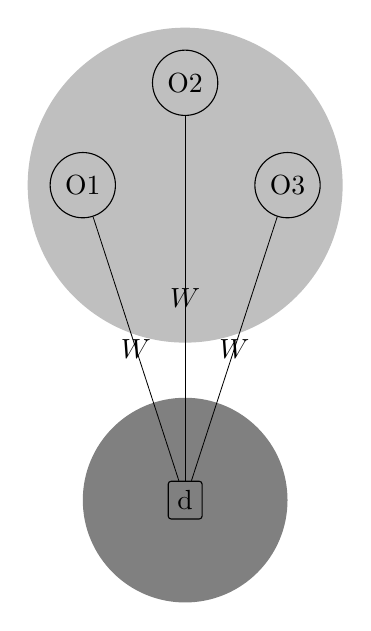
\begin{tikzpicture}
			\coordinate (ORI) at (0, 0);
			\coordinate (DEST) at (0, -4);
			\fill[lightgray] (ORI) circle(2);
			\fill[gray] (DEST) circle(1.3);
			\node[draw, circle, label=above:{$$}] (O1)at(-1.3, 0) {O1};
			\node[draw, circle, label=above:{$$}] (O2)at(0, 1.3) {O2};
			\node[draw, circle, label=above:{$$}] (O3)at(1.3, 0) {O3};
			\node[draw, rectangle, rounded corners=1pt, fill=gray!100, label=above:{$$}] (D)at(0, -4) {d};
			\draw[line width=0.3pt] (O1) -- (D) node[midway] {$W$};
			\draw[line width=0.3pt] (O2) -- (D) node[midway] {$W$};
			\draw[line width=0.3pt] (O3) -- (D) node[midway] {$W$};
		\end{tikzpicture}
		\caption{Distance between origins and destinations W}
		\label{fig:Distance between origins and destinations W}
	\end{figure}
	
	\noindent In the Figure \ref{fig:Distance between origins and destinations W} is represented the distance $W$, which is the same regardless of origin.
	\newpar
	In order to prove that the CPP is NP-hard, we must prove the following equivalence: \newline
	\textbf{I} is a yes-instance for the HPP \textit{is equivalent to} \textbf{I'} is a yes-instance for the CPP.
	
	\subsection{Proof of one way}
	\label{subsec:Proof of one way}
	
	Let's prove it in the way \textbf{I} is a yes-instance for the HPP if \textbf{I'} is a yes-instance for the CPP.
	
	\begin{figure}[H]
		\centering
		\begin{subfigure}{.5\textwidth}
			\centering
			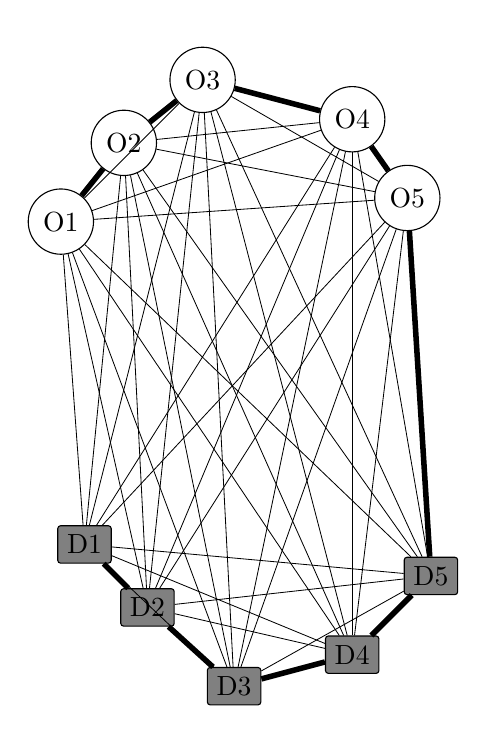
\begin{tikzpicture}
				\node[draw, circle, label=above:{$$}] (A)at(-2.8, -0.5) {O1};	
				\node[draw, circle, label=above:{$$}] (B)at(-2, 0.5) {O2};
				\node[draw, circle, label=above:{$$}] (C)at(-1, 1.3) {O3};
				\node[draw, circle, label=above:{$$}] (D)at(0.9, 0.8) {O4};
				\node[draw, circle, label=above:{$$}] (E)at(1.6, -0.2) {O5};
				\node[draw, rectangle, rounded corners=1pt, fill=gray!100, label=above:{$$}] (WA)at(-2.5, -4.6) {D1};
				\node[draw, rectangle, rounded corners=1pt, fill=gray!100, label=above:{$$}] (WB)at(-1.7, -5.4) {D2};	
				\node[draw, rectangle, rounded corners=1pt, fill=gray!100, label=above:{$$}] (WC)at(-0.6, -6.4) {D3};
				\node[draw, rectangle, rounded corners=1pt, fill=gray!100, label=above:{$$}] (WD)at(0.9, -6) {D4};
				\node[draw, rectangle, rounded corners=1pt, fill=gray!100, label=above:{$$}] (WE)at(1.9, -5) {D5};
				\draw[line width=2pt] (A) -- (B) node[midway] {$$};
				\draw[line width=0.3pt] (A) -- (C) node[midway] {$$};
				\draw[line width=0.3pt] (A) -- (D) node[midway] {$$};
				\draw[line width=0.3pt] (A) -- (E) node[midway] {$$};
				\draw[line width=2pt] (B) -- (C) node[midway] {$$};
				\draw[line width=0.3pt] (B) -- (D) node[midway] {$$};
				\draw[line width=0.3pt] (B) -- (E) node[midway] {$$};
				\draw[line width=2pt] (C) -- (D) node[midway] {$$};
				\draw[line width=0.3pt] (C) -- (E) node[midway] {$$};
				\draw[line width=2pt] (D) -- (E) node[midway] {$$};
				\draw[line width=0.3pt] (WA) -- (A) node[midway] {$$};
				\draw[line width=0.3pt] (WA) -- (B) node[midway] {$$};
				\draw[line width=0.3pt] (WA) -- (C) node[midway] {$$};
				\draw[line width=0.3pt] (WA) -- (D) node[midway] {$$};
				\draw[line width=0.3pt] (WA) -- (E) node[midway] {$$};
				\draw[line width=0.3pt] (WB) -- (A) node[midway] {$$};
				\draw[line width=0.3pt] (WB) -- (B) node[midway] {$$};	
				\draw[line width=0.3pt] (WB) -- (C) node[midway] {$$};
				\draw[line width=0.3pt] (WB) -- (D) node[midway] {$$};
				\draw[line width=0.3pt] (WB) -- (E) node[midway] {$$};
				\draw[line width=0.3pt] (WC) -- (A) node[midway] {$$};
				\draw[line width=0.3pt] (WC) -- (B) node[midway] {$$};
				\draw[line width=0.3pt] (WC) -- (C) node[midway] {$$};
				\draw[line width=0.3pt] (WC) -- (D) node[midway] {$$};
				\draw[line width=0.3pt] (WC) -- (E) node[midway] {$$};
				\draw[line width=0.3pt] (WD) -- (A) node[midway] {$$};
				\draw[line width=0.3pt] (WD) -- (B) node[midway] {$$};
				\draw[line width=0.3pt] (WD) -- (C) node[midway] {$$};
				\draw[line width=0.3pt] (WD) -- (D) node[midway] {$$};
				\draw[line width=0.3pt] (WD) -- (E) node[midway] {$$};
				\draw[line width=0.3pt] (WE) -- (A) node[midway] {$$};
				\draw[line width=0.3pt] (WE) -- (B) node[midway] {$$};
				\draw[line width=0.3pt] (WE) -- (C) node[midway] {$$};
				\draw[line width=0.3pt] (WE) -- (D) node[midway] {$$};
				\draw[line width=2pt] (WE) -- (E) node[midway] {$$};
				\draw[line width=2pt] (WE) -- (WD) node[midway] {$$};
				\draw[line width=0.3pt] (WE) -- (WC) node[midway] {$$};
				\draw[line width=0.3pt] (WE) -- (WB) node[midway] {$$};
				\draw[line width=0.3pt] (WE) -- (WA) node[midway] {$$};
				\draw[line width=2pt] (WD) -- (WC) node[midway] {$$};
				\draw[line width=0.3pt] (WD) -- (WB) node[midway] {$$};
				\draw[line width=0.3pt] (WD) -- (WA) node[midway] {$$};
				\draw[line width=2pt] (WC) -- (WB) node[midway] {$$};
				\draw[line width=0.3pt] (WC) -- (WA) node[midway] {$$};
				\draw[line width=2pt] (WB) -- (WA) node[midway] {$$};
			\end{tikzpicture}
			\caption{A solution of an Instance I in the CPP}
		\end{subfigure}%
		\begin{subfigure}{.5\textwidth}
			\centering
			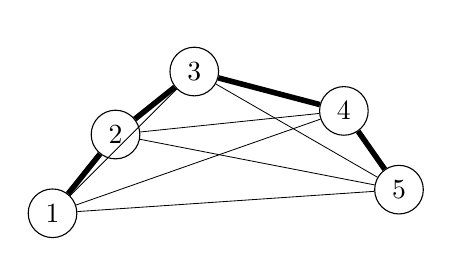
\begin{tikzpicture}
				\node[draw, circle, label=above:{$$}] (A)at(-2.8, -0.5) {1};	
				\node[draw, circle, label=above:{$$}] (B)at(-2, 0.5) {2};
				\node[draw, circle, label=above:{$$}] (C)at(-1, 1.3) {3};
				\node[draw, circle, label=above:{$$}] (D)at(0.9, 0.8) {4};
				\node[draw, circle, label=above:{$$}] (E)at(1.6, -0.2) {5};
				\draw[line width=2pt] (A) -- (B) node[midway] {$$};
				\draw[line width=0.3pt] (A) -- (C) node[midway] {$$};
				\draw[line width=0.3pt] (A) -- (D) node[midway] {$$};
				\draw[line width=0.3pt] (A) -- (E) node[midway] {$$};
				\draw[line width=2pt] (B) -- (C) node[midway] {$$};
				\draw[line width=0.3pt] (B) -- (D) node[midway] {$$};
				\draw[line width=0.3pt] (B) -- (E) node[midway] {$$};
				\draw[line width=2pt] (C) -- (D) node[midway] {$$};
				\draw[line width=0.3pt] (C) -- (E) node[midway] {$$};
				\draw[line width=2pt] (D) -- (E) node[midway] {$$};
			\end{tikzpicture}
			\caption{A solution of an Instance I' in the HPP}
		\end{subfigure}
		\caption{Example of a solution to CPP in the HPP}
		\label{fig:Example of a solution to CPP in the HPP}
	\end{figure}
	
	If we only have one car and remove the Origin-Destination W trip, then our CPP solution are HPP solutions as shown in Figure \ref{fig:Example of a solution to CPP in the HPP}.
	\newpar
	Our instances of the CPP can only have \textbf{one vehicle} as a solution:\newline
	Let's see the case where there are two vehicles going to the destinations.\newline
	If we take two vehicles then we have in our solution at least twice the distance $W$.\newline
	We know $B<W$, then we have $B'\ge 2W>W+B$, and that's impossible because $B'=W+B$. \newline
	This counterexample proves that we can only have one vehicle traveling all the vertices.
	\newpar
	Moreover, we have to prove this is the same solution to minimize weight in both problems.\newline
	As we know that each origin is exactly at the distance $W$ of destinations, no matter the place of origin chosen to go to destination, we will add $W$ to it.\newline
	So minimizing $B'$ is equivalent to minimize the distance between the origins $B$.\newline
	We proved \textbf{I} is a yes-instance for the HPP if \textbf{I'} is a yes-instance for the CPP.
	
	\subsection{Proof in the other way}
	
	Now that we have proved a way, let's prove that \textbf{I'} is a yes-instance for the CPP if and only if \textbf{I} is a yes-instance for the HPP.\newline
	Let's take a solution of the HPP. If we add an edge from one of the extremities of the path to the destination, then we have a solution for the CPP. \newline
	The choice of the added edge does not change anything to the solution since each origin is at equal distance $W$ from the destinations. It must be at one extremity to comply with the CPP. \newline
	As far as the number of vehicles is concerned, there can only be one since $B'=W+B$, as shown  in section \ref{subsec:Proof of one way}.
	\newpar
	Now let's see if other constraints added to the problem influence the complexity.
	
	%%%%%%%%%%%%%%%% OTHER CARACTERISTICS %%%%%%%%%%%%%%%%%%%%%%%
	\subsection{Other characteristics}
	
	\subsubsection{Time windows}
	
	The time windows associated with each vertex is not a problem because we can recreate any HPP instances where these constraints do not change the complexity of the problem.
	
	\begin{figure}[H]
		\centering
		\begin{subfigure}{.5\textwidth}
			\centering
			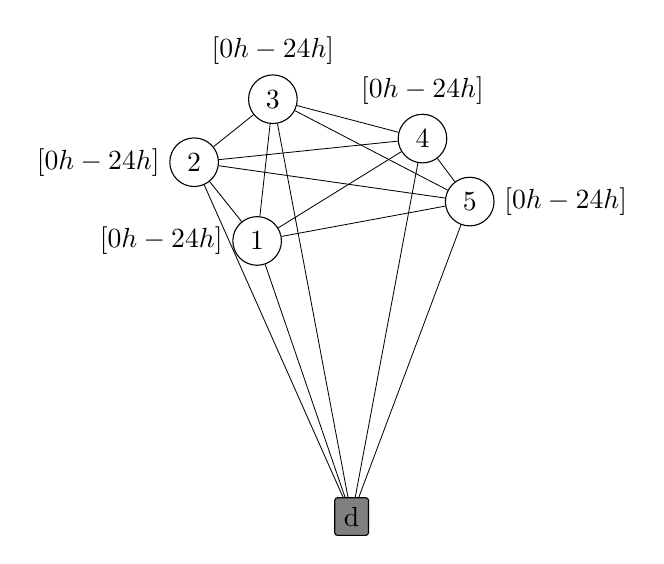
\begin{tikzpicture}
				\node[draw, circle, label=left:{$[0h-24h]$}] (A)at(-1.2, -0.5) {1};
				\node[draw, circle, label=left:{$[0h-24h]$}] (B)at(-2, 0.5) {2};
				\node[draw, circle, label=above:{$[0h-24h]$}] (C)at(-1, 1.3) {3};
				\node[draw, circle, label=above:{$[0h-24h]$}] (D)at(0.9, 0.8) {4};
				\node[draw, circle, label=right:{$[0h-24h]$}] (E)at(1.5, 0) {5};
				\node[draw, rectangle, rounded corners=1pt, fill=gray!100, label=above:{$$}] (W)at(0, -4) {d};
				\draw[line width=0.3pt] (A) -- (B) node[midway] {$$};
				\draw[line width=0.3pt] (A) -- (C) node[midway] {$$};
				\draw[line width=0.3pt] (A) -- (D) node[midway] {$$};
				\draw[line width=0.3pt] (A) -- (E) node[midway] {$$};
				\draw[line width=0.3pt] (B) -- (C) node[midway] {$$};
				\draw[line width=0.3pt] (B) -- (D) node[midway] {$$};
				\draw[line width=0.3pt] (B) -- (E) node[midway] {$$};
				\draw[line width=0.3pt] (C) -- (D) node[midway] {$$};
				\draw[line width=0.3pt] (C) -- (E) node[midway] {$$};
				\draw[line width=0.3pt] (D) -- (E) node[midway] {$$};
				\draw[line width=0.3pt] (W) -- (A) node[midway] {$$};
				\draw[line width=0.3pt] (W) -- (B) node[midway] {$$};
				\draw[line width=0.3pt] (W) -- (C) node[midway] {$$};
				\draw[line width=0.3pt] (W) -- (D) node[midway] {$$};
				\draw[line width=0.3pt] (W) -- (E) node[midway] {$$};
			\end{tikzpicture}
			\caption{Vertices of the instance}
		\end{subfigure}%
		\begin{subfigure}{.5\textwidth}
			\centering
			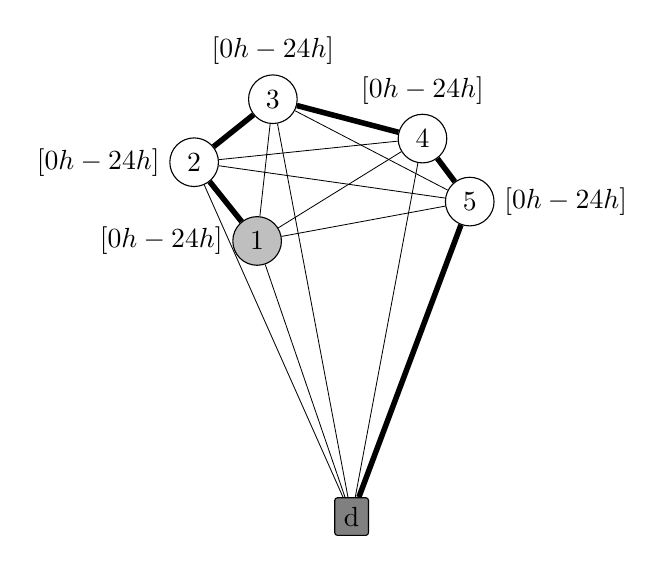
\begin{tikzpicture}
				\node[draw, fill=gray!50, circle, label=left:{$[0h-24h]$}] (A)at(-1.2, -0.5) {1};
				\node[draw, circle, label=left:{$[0h-24h]$}] (B)at(-2, 0.5) {2};
				\node[draw, circle, label=above:{$[0h-24h]$}] (C)at(-1, 1.3) {3};
				\node[draw, circle, label=above:{$[0h-24h]$}] (D)at(0.9, 0.8) {4};
				\node[draw, circle, label=right:{$[0h-24h]$}] (E)at(1.5, 0) {5};
				\node[draw, rectangle, rounded corners=1pt, fill=gray!100, label=above:{$$}] (W)at(0, -4) {d};
				\draw[line width=2pt] (A) -- (B) node[midway] {$$};
				\draw[line width=0.3pt] (A) -- (C) node[midway] {$$};
				\draw[line width=0.3pt] (A) -- (D) node[midway] {$$};
				\draw[line width=0.3pt] (A) -- (E) node[midway] {$$};
				\draw[line width=2pt] (B) -- (C) node[midway] {$$};
				\draw[line width=0.3pt] (B) -- (D) node[midway] {$$};
				\draw[line width=0.3pt] (B) -- (E) node[midway] {$$};
				\draw[line width=2pt] (C) -- (D) node[midway] {$$};
				\draw[line width=0.3pt] (C) -- (E) node[midway] {$$};
				\draw[line width=2pt] (D) -- (E) node[midway] {$$};
				\draw[line width=0.3pt] (W) -- (A) node[midway] {$$};
				\draw[line width=0.3pt] (W) -- (B) node[midway] {$$};
				\draw[line width=0.3pt] (W) -- (C) node[midway] {$$};
				\draw[line width=0.3pt] (W) -- (D) node[midway] {$$};
				\draw[line width=2pt] (W) -- (E) node[midway] {$$};
			\end{tikzpicture}
			\caption{A solution}
		\end{subfigure}
		\caption{CPP with time windows}
		\label{fig:CPP with time windows}
	\end{figure}
	
	By leaving the free schedules as in this instance \ref{fig:CPP with time windows}, we prove that an instance of the problem is NP-hard.
	
	\subsubsection{Return management}
	
	Take the instance of the Figure \ref{fig:CPP with time windows}, we can imagine that the solution of return can be the same solution as to the opposite way, which proves that the complexity remains unchanged.
	
	\subsubsection{Different return locations}
	
	Let's take an example where the return is totally different.
	
	\begin{figure}[H]
		\centering
		\begin{subfigure}{.5\textwidth}
			\centering
			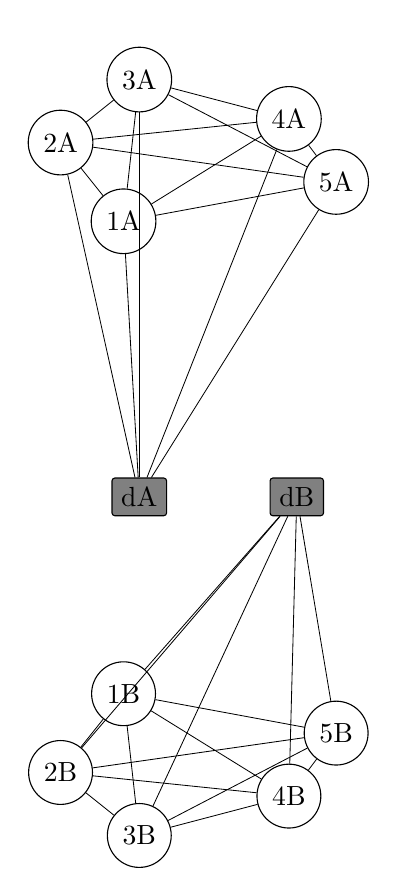
\begin{tikzpicture}
				\node[draw, circle, label=above:{$$}] (A)at(-1.2, -0.5) {1A};
				\node[draw, circle, label=above:{$$}] (B)at(-2, 0.5) {2A};
				\node[draw, circle, label=above:{$$}] (C)at(-1, 1.3) {3A};
				\node[draw, circle, label=above:{$$}] (D)at(0.9, 0.8) {4A};
				\node[draw, circle, label=above:{$$}] (E)at(1.5, 0) {5A};
				\node[draw, rectangle, rounded corners=1pt, fill=gray!100, label=above:{$$}] (W)at(-1, -4) {dA};
				\node[draw, circle, label=above:{$$}] (A2)at(-1.2, -6.5) {1B};
				\node[draw, circle, label=above:{$$}] (B2)at(-2, -7.5) {2B};
				\node[draw, circle, label=above:{$$}] (C2)at(-1, -8.3) {3B};
				\node[draw, circle, label=above:{$$}] (D2)at(0.9, -7.8) {4B};
				\node[draw, circle, label=above:{$$}] (E2)at(1.5, -7) {5B};
				\node[draw, rectangle, rounded corners=1pt, fill=gray!100, label=above:{$$}] (W2)at(1, -4) {dB};
				\draw[line width=0.3pt] (A) -- (B) node[midway] {$$};
				\draw[line width=0.3pt] (A) -- (C) node[midway] {$$};
				\draw[line width=0.3pt] (A) -- (D) node[midway] {$$};
				\draw[line width=0.3pt] (A) -- (E) node[midway] {$$};
				\draw[line width=0.3pt] (B) -- (C) node[midway] {$$};
				\draw[line width=0.3pt] (B) -- (D) node[midway] {$$};
				\draw[line width=0.3pt] (B) -- (E) node[midway] {$$};
				\draw[line width=0.3pt] (C) -- (D) node[midway] {$$};
				\draw[line width=0.3pt] (C) -- (E) node[midway] {$$};
				\draw[line width=0.3pt] (D) -- (E) node[midway] {$$};
				\draw[line width=0.3pt] (W) -- (A) node[midway] {$$};
				\draw[line width=0.3pt] (W) -- (B) node[midway] {$$};
				\draw[line width=0.3pt] (W) -- (C) node[midway] {$$};
				\draw[line width=0.3pt] (W) -- (D) node[midway] {$$};
				\draw[line width=0.3pt] (W) -- (E) node[midway] {$$};
				\draw[line width=0.3pt] (A2) -- (B2) node[midway] {$$};
				\draw[line width=0.3pt] (A2) -- (C2) node[midway] {$$};
				\draw[line width=0.3pt] (A2) -- (D2) node[midway] {$$};
				\draw[line width=0.3pt] (A2) -- (E2) node[midway] {$$};
				\draw[line width=0.3pt] (B2) -- (C2) node[midway] {$$};
				\draw[line width=0.3pt] (B2) -- (D2) node[midway] {$$};
				\draw[line width=0.3pt] (B2) -- (E2) node[midway] {$$};
				\draw[line width=0.3pt] (C2) -- (D2) node[midway] {$$};
				\draw[line width=0.3pt] (C2) -- (E2) node[midway] {$$};
				\draw[line width=0.3pt] (D2) -- (E2) node[midway] {$$};
				\draw[line width=0.3pt] (W2) -- (A2) node[midway] {$$};
				\draw[line width=0.3pt] (W2) -- (B2) node[midway] {$$};
				\draw[line width=0.3pt] (W2) -- (C2) node[midway] {$$};
				\draw[line width=0.3pt] (W2) -- (D2) node[midway] {$$};
				\draw[line width=0.3pt] (W2) -- (E2) node[midway] {$$};
			\end{tikzpicture}
			\caption{Vertices of the instance}
		\end{subfigure}%
		\begin{subfigure}{.5\textwidth}
			\centering
			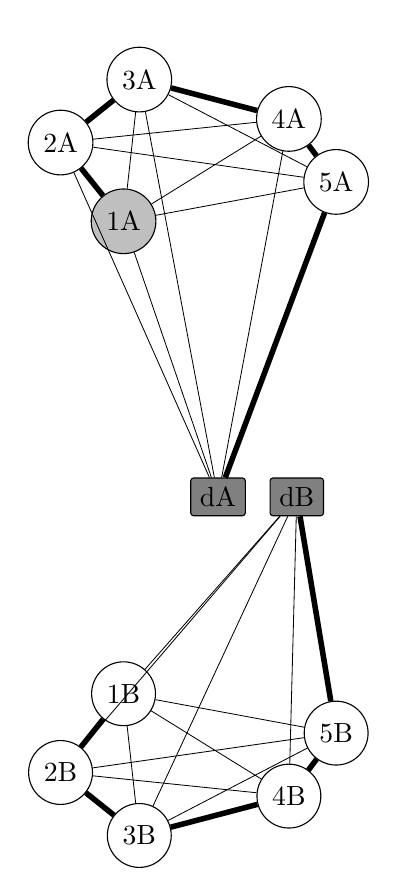
\begin{tikzpicture}
				\node[draw, fill=gray!50, circle, label=above:{$$}] (A)at(-1.2, -0.5) {1A};
				\node[draw, circle, label=above:{$$}] (B)at(-2, 0.5) {2A};
				\node[draw, circle, label=above:{$$}] (C)at(-1, 1.3) {3A};
				\node[draw, circle, label=above:{$$}] (D)at(0.9, 0.8) {4A};
				\node[draw, circle, label=above:{$$}] (E)at(1.5, 0) {5A};
				\node[draw, rectangle, rounded corners=1pt, fill=gray!100, label=above:{$$}] (W)at(0, -4) {dA};
				\node[draw, circle, label=above:{$$}] (A2)at(-1.2, -6.5) {1B};
				\node[draw, circle, label=above:{$$}] (B2)at(-2, -7.5) {2B};
				\node[draw, circle, label=above:{$$}] (C2)at(-1, -8.3) {3B};
				\node[draw, circle, label=above:{$$}] (D2)at(0.9, -7.8) {4B};
				\node[draw, circle, label=above:{$$}] (E2)at(1.5, -7) {5B};
				\node[draw, rectangle, rounded corners=1pt, fill=gray!100, label=above:{$$}] (W2)at(1, -4) {dB};
				\draw[line width=2pt] (A) -- (B) node[midway] {$$};
				\draw[line width=0.3pt] (A) -- (C) node[midway] {$$};
				\draw[line width=0.3pt] (A) -- (D) node[midway] {$$};
				\draw[line width=0.3pt] (A) -- (E) node[midway] {$$};
				\draw[line width=2pt] (B) -- (C) node[midway] {$$};
				\draw[line width=0.3pt] (B) -- (D) node[midway] {$$};
				\draw[line width=0.3pt] (B) -- (E) node[midway] {$$};
				\draw[line width=2pt] (C) -- (D) node[midway] {$$};
				\draw[line width=0.3pt] (C) -- (E) node[midway] {$$};
				\draw[line width=2pt] (D) -- (E) node[midway] {$$};
				\draw[line width=0.3pt] (W) -- (A) node[midway] {$$};
				\draw[line width=0.3pt] (W) -- (B) node[midway] {$$};
				\draw[line width=0.3pt] (W) -- (C) node[midway] {$$};
				\draw[line width=0.3pt] (W) -- (D) node[midway] {$$};
				\draw[line width=2pt] (W) -- (E) node[midway] {$$};
				\draw[line width=2pt] (A2) -- (B2) node[midway] {$$};
				\draw[line width=0.3pt] (A2) -- (C2) node[midway] {$$};
				\draw[line width=0.3pt] (A2) -- (D2) node[midway] {$$};
				\draw[line width=0.3pt] (A2) -- (E2) node[midway] {$$};
				\draw[line width=2pt] (B2) -- (C2) node[midway] {$$};
				\draw[line width=0.3pt] (B2) -- (D2) node[midway] {$$};
				\draw[line width=0.3pt] (B2) -- (E2) node[midway] {$$};
				\draw[line width=2pt] (C2) -- (D2) node[midway] {$$};
				\draw[line width=0.3pt] (C2) -- (E2) node[midway] {$$};
				\draw[line width=2pt] (D2) -- (E2) node[midway] {$$};
				\draw[line width=0.3pt] (W2) -- (A2) node[midway] {$$};
				\draw[line width=0.3pt] (W2) -- (B2) node[midway] {$$};
				\draw[line width=0.3pt] (W2) -- (C2) node[midway] {$$};
				\draw[line width=0.3pt] (W2) -- (D2) node[midway] {$$};
				\draw[line width=2pt] (W2) -- (E2) node[midway] {$$};
			\end{tikzpicture}
			\caption{A solution}
		\end{subfigure}
		\caption{CPP with different return locations}
		\label{fig:CPP with different return locations}
	\end{figure}
	
	We can break down the problem into two sub-problems corresponding both to the Hamiltonian Path Problem. So the complexity remains NP-Hard.
	
	%%%%%%%% %%%%%%%% %%%%%%%%
	%%%%%%%% SOLVING MODEL %%%%%%%%
	%%%%%%%%% %%%%%%%% %%%%%%%
	\cleardoublepage
	\chapter{Problem solving model}
	
	In this chapter we will see our choices of resolution, and how we have implemented these choices. 
	
	%%%%%%%%%%%% Resolution %%%%%%%%%%%% 
	\section{Resolution specificities}
	
	Here is a description and a comparison of how to solve the problem with different models. 
	
	\subsection{Different models}
	
	We have two types of models to implement in order to compare them: \newline
	Management of the return trip \textbf{associated} with the management of the home-to-work trip. \newline
	Management of the return trip \textbf{dissociated} with the management of the home-to-work trip.
	\newpar
	In other words, \textbf{dissociate} means that we have a model that manages the home-to-work trip, and another that manages the return, based on the outcome of the go, ie the results of the program for the go are part of the program data for the return. \textbf{Associate} means that our program manages all the trips directly with the starting dataset.
	\newpar
	For each of these two models, we have the case where the carpoolers are in the \textbf{same pool} for the home-to-work trip and the return trip, and the case where they can be in \textbf{different pools}
	\newpar
	Let's see some examples in the following content:
	\begin{figure}[H]
		\centering
		\begin{subfigure}{.5\textwidth}
			\centering
			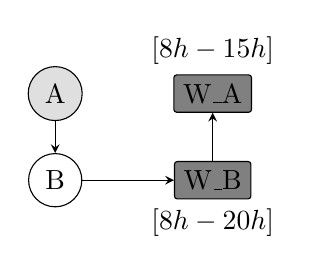
\begin{tikzpicture}
				\node[draw, circle, fill=gray!25, label=above:{$$}] (A)at(-1.5, 0.5) {A};
				\node[draw, circle, label=above:{$$}] (B)at(-1.5, -0.6) {B};
				\node[draw, rectangle, rounded corners=1pt, fill=gray!100, label=above:{$[8h-15h]$}] (WA)at(0.5, 0.5) {W\_A};
				\node[draw, rectangle, rounded corners=1pt, fill=gray!100, label=below:{$[8h-20h]$}] (WB)at(0.5, -0.6) {W\_B};
				\draw[->, >=stealth] (A) -- (B);
				\draw[->, >=stealth] (B) -- (WB);
				\draw[->, >=stealth] (WB) -- (WA);
			\end{tikzpicture}
			\caption{Home-to-work trip}
		\end{subfigure}%
		\begin{subfigure}{.5\textwidth}
			\centering
			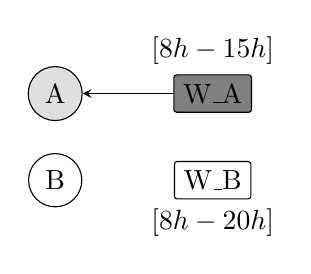
\begin{tikzpicture}
				\node[draw, circle, fill=gray!25, label=above:{$$}] (A)at(-1.5, 0.5) {A};
				\node[draw, circle, label=above:{$$}] (B)at(-1.5, -0.6) {B};
				\node[draw, rectangle, rounded corners=1pt, fill=gray!100, label=above:{$[8h-15h]$}] (WA)at(0.5, 0.5) {W\_A};
				\node[draw, rectangle, rounded corners=1pt, label=below:{$[8h-20h]$}] (WB)at(0.5, -0.6) {W\_B};
				\draw[->, >=stealth] (WA) -- (A);
			\end{tikzpicture}
			\caption{Return trip}
		\end{subfigure}
		\caption{Dissociated programs}
		\label{fig:dissociated programs}
	\end{figure}
	
	Figure \ref{fig:dissociated programs} represents two implemented dissociated model, where one is executed for the home-to-work trip, and the other one for the corresponding return trip. \newline
	We introduce the notion of people who are \textbf{left behind}. We can observe it in $(b)$, only taking into account the schedules of work's beginning, this is obvious that we take only one car to save some fuel. However at the return trip, there are five hours of difference in schedules when they end the work. The person who took his car can go back home whereas the person who has not taken his car is stuck at work. \newline
	Of course, someone else would be able to pick up this person on the return run if there were more requests, but if this is not the case, this person is in the \textbf{left behind group}.\newline
	During the execution of these two dissociated models, there will be the number of people \textbf{left behind} in the solution.
	
	\begin{figure}[H]
		\centering
		\begin{subfigure}{.5\textwidth}
			\centering
			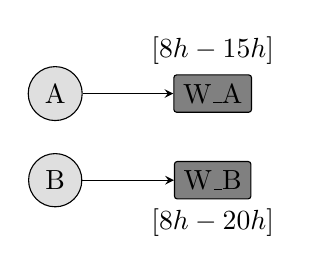
\begin{tikzpicture}
				\node[draw, circle, fill=gray!25, label=above:{$$}] (A)at(-1.5, 0.5) {A};
				\node[draw, circle, fill=gray!25, label=above:{$$}] (B)at(-1.5, -0.6) {B};
				\node[draw, rectangle, rounded corners=1pt, fill=gray!100, label=above:{$[8h-15h]$}] (WA)at(0.5, 0.5) {W\_A};
				\node[draw, rectangle, rounded corners=1pt, fill=gray!100, label=below:{$[8h-20h]$}] (WB)at(0.5, -0.6) {W\_B};
				\draw[->, >=stealth] (A) -- (WA);
				\draw[->, >=stealth] (B) -- (WB);
			\end{tikzpicture}
			\caption{Home-to-work trip}
		\end{subfigure}%
		\begin{subfigure}{.5\textwidth}
			\centering
			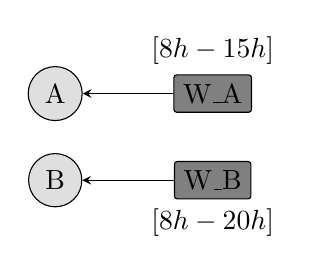
\begin{tikzpicture}
				\node[draw, circle, fill=gray!25, label=above:{$$}] (A)at(-1.5, 0.5) {A};
				\node[draw, circle, fill=gray!25, label=above:{$$}] (B)at(-1.5, -0.6) {B};
				\node[draw, rectangle, rounded corners=1pt, fill=gray!100, label=above:{$[8h-15h]$}] (WA)at(0.5, 0.5) {W\_A};
				\node[draw, rectangle, rounded corners=1pt, fill=gray!100, label=below:{$[8h-20h]$}] (WB)at(0.5, -0.6) {W\_B};
				\draw[->, >=stealth] (WA) -- (A);
				\draw[->, >=stealth] (WB) -- (B);
			\end{tikzpicture}
			\caption{Return trip}
		\end{subfigure}
		\caption{Associated programs}
		\label{fig:associated programs}
	\end{figure}
	
	Figure \ref{fig:associated programs} shows that with the same initial data as in the Figure \ref{fig:dissociated programs}, we have a different solution. Indeed, this time the management of the work and return to work are done at the same time, in the same system of decision support. So the solution for this one, knowing that on the return they will need theirs cars, is to take each their car at the start.
	\newpar
	The usefulness of having both types of models makes it possible to compare the execution times on the same number of users, as well as the value of solutions.
	
	\begin{figure}[H]
		\centering
		\begin{subfigure}{.5\textwidth}
			\centering
			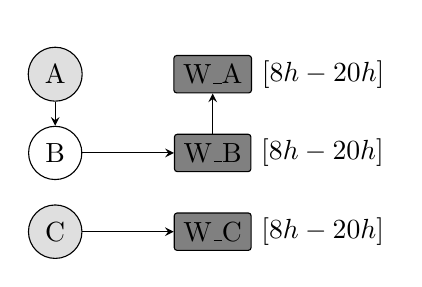
\begin{tikzpicture}
				\node[draw, circle, fill=gray!25, label=above:{$$}] (A)at(-1.5, 0.5) {A};
				\node[draw, circle, label=above:{$$}] (B)at(-1.5, -0.5) {B};
				\node[draw, circle, fill=gray!25, label=above:{$$}] (C)at(-1.5, -1.5) {C};
				\node[draw, rectangle, rounded corners=1pt, fill=gray!100, label=right:{$[8h-20h]$}] (WA)at(0.5, 0.5) {W\_A};
				\node[draw, rectangle, rounded corners=1pt, fill=gray!100, label=right:{$[8h-20h]$}] (WB)at(0.5, -0.5) {W\_B};
				\node[draw, rectangle, rounded corners=1pt, fill=gray!100, label=right:{$[8h-20h]$}] (WC)at(0.5, -1.5) {W\_C};
				\draw[->, >=stealth] (A) -- (B);
				\draw[->, >=stealth] (B) -- (WB);
				\draw[->, >=stealth] (WB) -- (WA);
				\draw[->, >=stealth] (C) -- (WC);
			\end{tikzpicture}
			\caption{Home-to-work trip}
		\end{subfigure}%
		\begin{subfigure}{.5\textwidth}
			\centering
			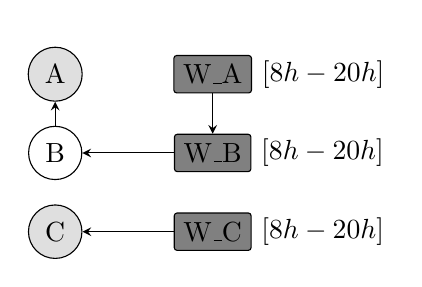
\begin{tikzpicture}
				\node[draw, circle, fill=gray!25, label=above:{$$}] (A)at(-1.5, 0.5) {A};
				\node[draw, circle, label=above:{$$}] (B)at(-1.5, -0.5) {B};
				\node[draw, circle, fill=gray!25, label=above:{$$}] (C)at(-1.5, -1.5) {C};
				\node[draw, rectangle, rounded corners=1pt, fill=gray!100, label=right:{$[8h-20h]$}] (WA)at(0.5, 0.5) {W\_A};
				\node[draw, rectangle, rounded corners=1pt, fill=gray!100, label=right:{$[8h-20h]$}] (WB)at(0.5, -0.5) {W\_B};
				\node[draw, rectangle, rounded corners=1pt, fill=gray!100, label=right:{$[8h-20h]$}] (WC)at(0.5, -1.5) {W\_C};
				\draw[->, >=stealth] (WA) -- (WB);
				\draw[->, >=stealth] (WB) -- (B);
				\draw[->, >=stealth] (B) -- (A);
				\draw[->, >=stealth] (WC) -- (C);
			\end{tikzpicture}
			\caption{Return trip}
		\end{subfigure}
		\caption{Same pools}
		\label{fig:same pools}
	\end{figure}
	
	In Figure \ref{fig:same pools} we can see that the system provides a solution to have the same pool of people in the home-to-work trip and in the return trip.
	
	\begin{figure}[H]
		\centering
		\begin{subfigure}{.5\textwidth}
			\centering
			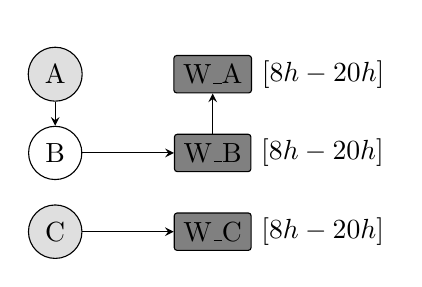
\begin{tikzpicture}
				\node[draw, circle, fill=gray!25, label=above:{$$}] (A)at(-1.5, 0.5) {A};
				\node[draw, circle, label=above:{$$}] (B)at(-1.5, -0.5) {B};
				\node[draw, circle, fill=gray!25, label=above:{$$}] (C)at(-1.5, -1.5) {C};
				\node[draw, rectangle, rounded corners=1pt, fill=gray!100, label=right:{$[8h-20h]$}] (WA)at(0.5, 0.5) {W\_A};
				\node[draw, rectangle, rounded corners=1pt, fill=gray!100, label=right:{$[8h-20h]$}] (WB)at(0.5, -0.5) {W\_B};
				\node[draw, rectangle, rounded corners=1pt, fill=gray!100, label=right:{$[8h-20h]$}] (WC)at(0.5, -1.5) {W\_C};
				\draw[->, >=stealth] (A) -- (B);
				\draw[->, >=stealth] (B) -- (WB);
				\draw[->, >=stealth] (WB) -- (WA);
				\draw[->, >=stealth] (C) -- (WC);
			\end{tikzpicture}
			\caption{Home-to-work trip}
		\end{subfigure}%
		\begin{subfigure}{.5\textwidth}
			\centering
			\begin{tikzpicture}
				\node[draw, circle, fill=gray!25, label=above:{$$}] (A)at(-1.5, 0.5) {A};
				\node[draw, circle, label=above:{$$}] (B)at(-1.5, -0.5) {B};
				\node[draw, circle, fill=gray!25, label=above:{$$}] (C)at(-1.5, -1.5) {C};
				\node[draw, rectangle, rounded corners=1pt, fill=gray!100, label=right:{$[8h-20h]$}] (WA)at(0.5, 0.5) {W\_A};
				\node[draw, rectangle, rounded corners=1pt, fill=gray!100, label=right:{$[8h-20h]$}] (WB)at(0.5, -0.5) {W\_B};
				\node[draw, rectangle, rounded corners=1pt, fill=gray!100, label=right:{$[8h-20h]$}] (WC)at(0.5, -1.5) {W\_C};
				\draw[->, >=stealth] (WA) -- (A);
				\draw[->, >=stealth] (WC) -- (WB);
				\draw[->, >=stealth] (WB) -- (B);
				\draw[->, >=stealth] (B) -- (C);
			\end{tikzpicture}
			\caption{Return trip}
		\end{subfigure}
		\caption{Different pools}
		\label{fig:different pools}
	\end{figure}
	
	Figure \ref{fig:different pools} shows that leaving pools open, ie they can be made different during the both trips, constraining less and leaving more solutions, by abandoning the stability emitted in the Figure \ref{fig:same pools}.
		
	\subsection{Heuristics used}
	
	\subsubsection{Finding satellites}
	During the study, we want to see the impact of the use of gathering places. Indeed, the places that we will call Satellites, can represent exits of motorway where to deposit people, to facilitate the movement of the users drivers. \newline
	The use of these satellites is done in data pre-management, where for example, people can be dropped on a motorway exit within 1 km of their work.\newline
	This use of satellite points makes it possible to have fewer destinations, since they will be, for some, gathered in these satellites.
	
	\subsubsection{Chose the data}
	
	Grenoble is surrounded by mountain ranges, a heuristic to gather the following data from where people come from works perfectly, and is an optimal solution since people would not have interest to go around the mountain ranges.
	
	\begin{figure}[H]
		\centering
		\begin{flushleft}
			\floatplacement{figure}{t}
			\includegraphics[scale=1]{img/i_grenoble.png}
		\end{flushleft}
		\caption{Mountains around Grenoble city}
		\label{fig:Mountains around Grenoble city}
	\end{figure}
	In Figure \ref{fig:Mountains around Grenoble city} the mountains are grayed and the blue arrows are rivers. This city configuration leaves only three major entrances, which are west, east and south. We can therefore create a group from each cardinality in order to increase the number of users taken into account by the decision system.
	\newpar
	We will now see which data are used by our models. 

	%%%%%%%%%%%%% DATA MODEL %%%%%%%%%%%% 
	\section{The data model}
	In this section, we will see the data are used by our models.
	
	\subsection{A representation in graph form}
	The requests and the travels can be represented by a directed graph $G=(V, A)$ where $V=\{1, ..., 4n\}$ is the set of Vertices and $A=\{arc(i, j) \forall i, j \in V\}$ is the set of Arcs. \newline
	All destinations of a person are shifted by $n$ from their first place. \newline
	For example the first user has the vertex pair $(1, 1+n)$ corresponding to his home-work trip vertices, and the vertex pair $(1+2n, 1+3n)$ corresponding to his return trip.

	\subsection{Sets range} 
	
	We have $n$ users, each one having four summits, two for the home-work trip and two for the return trip respectively. 
	
	\begin{tabbing}
		$O=\{1, ..., n\}$ \tab \tab \= Set of every possible driver/passenger. \\
		$D=\{n+1, ..., 2n\}$ \> Set of the workplaces. \\
		$U=O\cup D$ \> Set of home-to-work places. \\
	
		$K=\{2n+1, ..., 3n\}$ \> Set of the origins to return (may be the workplace). \\
		$L=\{3n+1, ..., 4n\}$ \> Set of the destinations to return (may be home). \\
		$W=K\cup L$ \> Set of return places. \\
	\end{tabbing}
	
	\subsection{Data used}
	In the dataset we have $C$ the cost matrix for moving from point i to point j represents either a distance, or a cost of gas, or a duration. $B$ and $E$ corresponds to the start and end time of the work, and $Q$ the capacity of the cars.
	
	\begin{tabbing}
		$C_{ij}$ \tab \= $\forall i, j\in V$ \tab \= Cost matrices for commuting $arc(i, j)$. \\
		
		$Q_{n}$ \> $\forall n\in O$ \> Car's capacity of the user $n$. \\
		
		$B_{v}$ \> $\forall v\in D$ \> Hour: Beginning of work for the user $n$. \\
		$E_{v}$ \> $\forall v\in K$ \> Hour: End of work for the user $n$. \\
		
		$\gamma$ \> \> Percentage of the initial travel time added to the max travel time. \\
		$\delta$ \> \> Constant value added to the max travel time. \\
		$\alpha$ \> \> Allowed waiting time to get to work early. \\
		$\beta$ \> \> Allowed waiting time to leave work. \\
		
		$M$ \> \> A large enough constant. \\
	\end{tabbing}
	
	\subsection{Diagram representation of data}
	
	In the following, the UML representation allows to visualize the data in another way.
	
	\begin{figure}[H]
		\centering
		\begin{flushleft}
			\floatplacement{figure}{t}
			\includegraphics[scale=0.7]{img/i_umlproblemdata.png}
		\end{flushleft}
		\caption{UML problem diagram}
		\label{fig:UML Diagram}
	\end{figure}
	
	\noindent Figure \ref{fig:UML Diagram} represents the data model. \newline
	The abstract class \textbf{Place} corresponds to the location of a place. Four classes inherit it, namely the place \textbf{MorningHome} that contains the capacity of the user's car, the place \textbf{MorningWorkplace} containing the time at which he starts work, the place \textbf{EveningWorkplace} containing the time at which his work ends, and the place \textbf{EveningHome} where he returns after work. Of course the workplaces can be the same, as well as the residential places. The \textbf{Travel(Arc)} class represents the arcs of the graph. This class takes two places to determine the time/distance between them. The \textbf{Request(Vertex)} class represents the vertices of the graph. This class takes the four places of the user's day in order to form a request composed of four vertices. The \textbf{SystemManager} class corresponds to what the person using the system must set for the mathematical model to work properly.
	
	\subsection{The dissociated models}
	
	The dissociated models have a first model taking the morning places, and a second model taking the evening places plus the result of those who take their cars in the first model.
	\newpar
	The next section discusses the mathematical model of the Mixed Integer linear Programs we have implemented to solve the problem.
	
	%%%%%%% MATHEMATICAL MODEL %%%%%%%
	\section{Mathematical modeling}
	
	We have binary variables representing the choices that must be made by the program, and variables representing sequencing, ie the time at which a driver would take a passenger, or the number of passengers inside. of this car after picking up or dropping people.
	
	\subsection{Decision variables}
	\begin{tabbing}
		$x^{k}_{ij}$ \tab \= $\forall k\in O, \forall i, j\in V$\tab \= $=1$ if the travel of the $arc(i, j)$ is deserved by the driver $k$. \\
		$y^{k}$ \> $\forall k\in O$ \> $=1$ if the user $k$ is a driver. \\
		$z^{k}_{v}$ \> $\forall k\in O, \forall v\in V$ \> $=1$ if the user $k$ is picking or delivering the vertex $v$. \\
		$b^{k}_{v}$ \> $\forall k\in O, \forall v\in V$ \> Estimated passage time of the driver $k$ to the vertex $v$. \\
		$q^{k}_{v}$ \> $\forall k\in O, \forall v\in V$ \> Number of persons in the car $k$ at the vertex $v$. \\
	\end{tabbing}
	
	We will now see what objectives our decision support system has. 
	
	\section{Objective functions}
	\[ Minimize \] 
	\begin{tabbing}
		$ \sum_{\substack{k\in O}}\sum_{\substack{i, j \in V}} C_{ij} \times x^{k}_{ij}$ \tab \tab \= The cost of all travels done \\
	\end{tabbing}
	
	Finally we will see the general and specific constraints of our models. For the sequencing constraints used in our models, we were inspired by Mr. Karimi \cite{karaoglanmemetic2015}, then we discovered a version of the more recent formula written by Mr. Karoaglan \cite{karimicapacitated2018}.
	
	\subsection{Constraints}
	\subsubsection{Path constraints}
	
	Each vertex haven't more than one outgoing arc.
	\[ \sum_{\substack{k\in O}}\sum_{\substack{j \in V, j\ne o}} x^{k}_{oj}\leq1 \tab \tab \forall o\in V \]
	
	Each vertex haven't more than one ingoing arc.
	\[ \sum_{\substack{k\in O}}\sum_{\substack{i \in V, i\ne d}} x^{k}_{id}\leq1 \tab \tab \forall d\in V \]
	
	A driver picks-up himself before picking up someone else, so he has two ingoing arc.
	\[ \sum_{\substack{j\in V}}x^{k}_{ij}\leq2\tab \tab \forall k\in O, \forall i\in V \]
	
	A passenger has only one destination after being picked-up.
	\[ \sum_{\substack{j\in V, j\ne k, j\ne k+2n}}x^{k}_{ij}\leq1\tab \tab \forall k\in O, \forall i\in V \]
	
	A driver is picking himself.
	\[ y^{k}=z^{k}_{k}\tab \tab \forall k\in O \]
	\[ y^{k}=x^{k}_{kk}\tab \tab \forall k\in O \]
	\[ x^{k}_{kk}=z^{k}_{k}\tab \tab \forall k\in O \]
	
	A non-driver can't pick himself.
	\[ x^{k}_{vv}=0 \tab \tab \forall k\in O, \forall v\in V, v\ne k, v\ne(k+2n)\]
	
	A vertex $v$ is taken at most by one and only one driver.
	\[ \sum_{\substack{k\in O}} z^{k}_{v}\leq1 \tab \tab \forall v\in V\]
	
	Prohibited cycles.
	\[ x^{k}_{ij}+x^{k}_{ji}\leq1\tab \tab \forall k\in O, \forall i\in V, \forall j\in U, i\ne j \]
	
	Each driver must reach their destination.
	\[ \sum_{\substack{k\in O}}\sum_{\substack{i \in V}} x^{k}_{id}=1 \tab \tab \forall d\in D\cup L \]
	
	Each driver must leave their home and their workplace. 
	\[ \sum_{\substack{k\in O}}\sum_{\substack{j \in V, j\ne o}} x^{k}_{oj}=1\tab \tab \forall o\in O \]

	If k is picking someone he delivers him at destination.
	\[ z^{k}_{o}==z^{k}_{o+n}\tab \tab \forall k\in O, o\in O\cup K \] 
	
	A driver never goes away from his destination.
	\[ \sum_{\substack{v\in D\cup v\in L}} x^{k}_{d, v}=0\tab \tab \forall k\in O \forall d=k+n\cup k+3n\]
	
	If $v$ is picked by $k$ then $k$ goes exactly one time to $v$.
	\[ z^{k}_{v}=\sum_{\substack{j\in U\cup W}} x^{k}_{vj} \tab \tab \forall k\in O, \forall v\in U\cup W \]
	
	\subsubsection{Time constraints}
	
	The sum of the travels of a driver $\leq$ maximum time allowed on the road for this user.
	\[ \sum_{\substack{i, j\in U\cup W}}x^{k}_{ij}\times C_{ij}\leq (1+\gamma \% )\times C_{k, k+n}+\delta \tab \tab \forall k\in O \]
	
	Sequencing the hours of passages.
	\[ b^{k}_{j}\geq b^{k}_{i}-B_{k+n}+(C_{ij}+B_{k+n})\times x^{k}_{ij}+(B_{k+n}-C_{ij})\times x^{k}_{ji}\tab \tab \forall k\in O, \forall i, j\in U, i\neq j \]
	\[ b^{k}_{j}\geq b^{k}_{i}-M+(C_{i-2n, j-2n}+M)\times x^{k}_{ij}+(M-C_{i-2n, j-2n})\times x^{k}_{ji}\tab \tab \forall k\in O, \forall i, j\in W, i\neq j \]
	
	Everyone arrives between $[B-\alpha , B]$.
	\[ \sum_{\substack{k\in O}}b^{k}_{v+n}\leq B_{v+n} \tab \tab \forall v\in O \]
	\[ \sum_{\substack{k\in O}}b^{k}_{v+n}\geq B_{v+n} - \alpha \tab \tab \forall v\in O \]
	
	Everyone leaves between $[arrival Time-MaximalTravelTime , arrival Time - C_{ij}]$.
	\[ \sum_{\substack{k\in O}}b^{k}_{v}\leq (\sum_{\substack{k\in O}} b^{k}_{v+n})- C_{v, v+n} \tab \tab \forall v\in O \]
	\[ \sum_{\substack{k\in O}}b^{k}_{v}\geq (\sum_{\substack{k\in O}} b^{k}_{v+n})- ((1+\gamma \% )\times C_{k, k+n}+\delta ) \tab \tab \forall v\in O \]
	
	Passage time is zero if vertex is not chosen.
	\[ b^{k}_{s}\leq z^{k}_{v}\times M \tab \tab \forall k\in O, \forall v\in V \] 
	
	\subsubsection{Capacity constraints}
	
	Each passenger can be in a car. 
	\[ \sum_{\substack{k\in O}}y^{k}\times Q_{k}\geq n \] 
	
	A driver k is his first passenger.
	\[ q_{k}^{k}=y^{k}\tab \tab \forall k\in O \] 
	
	Sequencing the number of passengers after visiting a vertex.
	\[ q_{k}^{j}\ge q_{k}^{i}-Q^{k}+(nPassengers_{j}+Q^{k})\times x^{k}_{ij}+(Q^{k}-nPassengers_{i})\times x^{k}_{ji} \]
	\[ \forall k\in O, \forall i\in U\cup W, \forall j\in U\cup W\]
	
	If a driver k visits the vertex i then his capacity after visiting it can't exceed the capacity of his car.
	\[ q_{k}^{v}\le Q^{k}\times z^{k}_{v}\tab \tab \forall k\in O, \forall v\in U\cup W \] 
	
	Return to home additional path constraints.\newline
	Each driver takes himself at the return.
	\[ x^{k-2n}_{kk}=y^{k-2n} \tab \tab \forall k\in K \] 
	
	\subsubsection{Same pool management}
	
	In order to have the same pool on the way back, we can force users picked-up from home-to-work trip to be picked-up by the same driver to the return trip.
	\[ z^{k}_{i}={k}_{i+2n} \tab \tab \forall k\in O, \forall i\in U \] 

	% USE
	\subsection{The use of the model}
	
	This mathematical model responds well to all the objectives that we set ourselves.

	Indeed, the places of the return trip may be different than home-to-work trip ones, and the hours of work are respected.
	
	We have access to the time values and capacity values at each vertex.
	
	\subsubsection{Limitations of the model}
	
	The number of users can not exceed thirty users because of the execution time which exponentially increases. The main cause is the management of sequencing, but it is necessary to not split it.
	\newpar
	We will now see how the experiments occurred.
	
	%%%%%%%%%%%% PROCESS %%%%%%%%%%%%
	\section{Resolution process}
	
	We have two execution processes for experiments. We define for each one a maximum execution time $x$ of the linear program, as well as a number of run to make $y$.
	
	\begin{figure}
		\centering
		\begin{flushleft}
			\floatplacement{figure}{t}
			\includegraphics[scale=0.6]{img/i_flowchartlpvariation.png}
		\end{flushleft}
		\caption{Flowchart of the LP's parameters variations}
		\label{fig:Flowchart of the LP variations}
	\end{figure}
	
	\noindent The first presented in Figure \ref{fig:Flowchart of the LP variations} shows the case where we keep the same instance and vary parameters of the linear program. 

	\noindent The second presented in the Figure \ref{fig:Flowchart of the problem's parameters variations} shows a parameter variation at the problem level. It is therefore necessary to renew the instance of the problem with these new parameters in order to take them into account.
	\newpar
	We will now see how these experiments unfolded.
	
	%%%%%%%% %%%%%%%% %%%%%%%%
	%%%%%%%% EXPERIMENTS %%%%%%%%
	%%%%%%%%% %%%%%%%% %%%%%%%
	\cleardoublepage
	\chapter{Experiments}
	
	We will see in each case which data we used, the value of the parameters, the results then we will analyze these results.
	
	\section{Experimental protocol}
	
	For all these experiments, we used the \textbf{CPLEX solver}. Our experimental platform is a computer with \textbf{8GB RAM memory}, an \textbf{Intel Core i5-4690 CPU 3.50 GHz}, and the operating system is \textbf{Windows 10 Professional 64-bit version}. The generator code and the solver code were written in \textbf{JAVA language}, and are available at the following address: \url{https://github.com/NeoKa4ra/CarPoolingInternship}.
	
	\section{About configurations}
	Here we will see how to understand the numbers given in the configurations. The JAVA lines of parameterization code being very explicit once understood, we will use them as configuration data throughout the experiments. In order to understand how this setting code works, we will detail each line of an example. \textbf{The car capacity of each user is always randomly between 2 and 4 seats}.
	\newpar
	\tab \textit{int nUsers = 5;}\newline
	The number of users.
	\newpar
	Before starting the next lines, it is necessary to define what is an experiment, a run and an execution. An experiment, called a run, is composed of several executions. The experience is therefore repeated over a number of run.\newline
	\tab // Usage:(modeLP, modeInstance, numberofRun, execInstanceTimeMax, execTotalTimeMax, nMaxUsers, suffix)\newline
	\tab \textit{GS = new GlobalSettings(Constants.GLPWR, Constants.GDI, 10, 300, 6, 12, "varyUsersWR");}\newline
	Here we have the parameters for the selected linear program, the instance mode, i.e. whether it is renewed between each execution or not, the number of runs of the experiment, the maximum time of an execution that stops the program if it is exceeded, the maximum total time that stops the execution if it is exceeded, the maximum number of users that stops the execution if it is reached, and a callsign for the test and result files. 
	\newpar
	We enter the two parameters of the instance, those concerning the time and those concerning the matrix. They have been separated to have fewer parameters on a single line, to improve understanding.
	\newpar
	\tab \textit{// (matrixMode, nbPersons, matrixRange, citiesList, workplacesList, probScdWork, probScdHome)}\newline
	\tab \textit{MS = new MatriceSettings(Constants.MCPWP, nUsers, 200, cities, workplaces, 20, 5);}\newline
	We have the matrix mode we want to have (completely random, etc.), the number of users, the range of each random instance of the matrix, the list of city coordinates, then work location coordinates, the probability of having a second job and the probability of having a second home.
	\newpar
	\tab \textit{// Usage:(nPersons, morningHour, morningHourRange, eveningHour, eveningHourRange)}\newline
	\tab \textit{HS = new HoursSettings(nUsers, 850, 50, 1500, 500);}\newline
	We have the number of users, the interval in which the working time must be in the morning, then the interval in which the working time must be in the evening. Note that the hours are in percentage of hours for simplicity's sake, 50 units corresponding to 50\% of one hour, i.e. 30 minutes.
	\newpar
	\tab \textit{// Usage:LPSettings(advance, waitingTime, deviationPercentage, deviationValue)}\newline
	\tab \textit{LPS = new LPSettings(50, 25, 20, 20);}\newline
	We have the maximum advance time to get to work, the longest waiting time after work, the percentage of deviation allowed and the fixed value of deviation allowed.
	\newpar
	\tab \textit{// (varyNUsers, varyAdvance, varyWaitingTime, varyDeviationPercentage, varyDeviationValue)}\newline
	\tab \textit{LPVS = new LPVariationsSettings(1, 0, 0, 0, 0);}\newline
	Here we have all possible variations for the parameters of the linear program, each number corresponds to the incrementation made between each execution.
	
	%%%%%%%%%%%%%%%%%%%% Variations in LP parameters %%%%%%%%%%%%%%%%%%%
	\section{Variations in LP parameters \& users}
	
	In this section, we will see how the objective and the execution time behave according to the variation of the linear program parameters.
	
	\subsection{Benchmarks}
	For the first tests, we used a distance matrix filled \textbf{randomly} in a range from 0 to 200, we will call it "All random" when it is filled completely randomly and "Random close homes" when the random is oriented so that people are closer to each other, as well as workplaces.
	
	\subsection{Configuration}
	Here are the parameters used in the following experiments.
	\newpar
	\tab \textit{int nUsers = x;}\newline
	The number of users.
	\newpar
	\tab \textit{// Usage:(modeLP, modeInstance, numberofRun, execInstanceTimeMax, execTotalTimeMax, nMaxUsers, suffix)}\newline
	\tab \textit{GS = new GlobalSettings(Constants.GLPWR, Constants.GSI, y, 300, 6, 25, "");}\newline
	The execution was done on the \textbf{linear program including the return path}, with the same instance at each run. The execution time was \textbf{300 seconds} maximum and the \textbf{total time was 6 minutes}. We had either \textbf{10 runs per experiment or 20}.
	\newpar
	\tab \textit{// (matrixMode, nbPersons, matrixRange, citiesList, workplacesList, probScdWork, probScdHome)}\newline
	\tab \textit{MS = new MatriceSettings(Constants.MM, nUsers, 200, cities, workplaces, 0, 0);}\newline
	The data were generated randomly, refer to benchmark. 
	\newpar
	\tab \textit{// Usage:(nPersons, morningHour, morningHourRange, eveningHour, eveningHourRange)}\newline
	\tab \textit{HS = new HoursSettings(nUsers, 850, 50, 1500, 500);}\newline
	Working hours were between \textbf{8:30 and 9:00 in the morning} and between \textbf{15:00 and 20:00 in the evening}.
	\newpar
	\tab \textit{// Usage:LPSettings(advance, waitingTime, deviationPercentage, deviationValue)}\newline
	\tab \textit{LPS = new LPSettings(50, 25, 20, 20);}\newline
	When one parameter varied, the others were always set to the base value indicated above. 
	\newpar
	\tab \textit{// (varyNUsers, varyAdvance, varyWaitingTime, varyDeviationPercentage, varyDeviationValue)}\newline
	\tab \textit{LPVS = new LPVariationsSettings(0, 1, 1, 1, 1);}\newline
	When a parameter varies, it is first set to zero and then incremented at each execution. Here we have all possible variations for the parameters of the linear program, each number corresponds to the incrementation made between each execution. We will see the variation on these parameters.

	\subsection{Results}
	As all the behaviors were similar, we studied one and put the results of this experiment in the appendix, see \ref{app:Continuation of the results of the LP parameter variations}.
	%%%%%%%%%%%%%%%%%%%%%%%%%%%% PERCENTAGE %%%%%%%%%%%%%%%%%%%%%%%%%%%
	\subsubsection{Varying the deviation's percentage of the travel allowed}

	\begin{figure}[H]
		\centering
		\begin{flushleft}
			\floatplacement{figure}{t}
			\includegraphics[scale=0.9]{img/compiledResults/4.png}
		\end{flushleft}
		\caption{Vary the deviation percentage with all random and with 20 users}
		\label{fig:Vary the deviation percentage with all random and with 20 users}
	\end{figure}

	In the Figure \ref{fig:Vary the deviation percentage with all random and with 20 users} we can see that the objective values remain the same regardless of the percentage deviation allowed, up to a maximum of 50\% . The execution time increases with the percentage of deviation.
	
	\begin{figure}[H]
		\centering
		\begin{flushleft}
			\floatplacement{figure}{t}
			\includegraphics[scale=0.9]{img/compiledResults/7.png}
		\end{flushleft}
		\caption{Vary the deviation percentage with random close homes and with 19 users}
		\label{fig:Vary the deviation percentage with random close homes and with 19 users}
	\end{figure}
	
	In the Figure \ref{fig:Vary the deviation percentage with random close homes and with 19 users}, we can see that the objective value decreases with the percentage deviation while the execution time tends to increase.
	
	\subsection{Analysis}
	The test for all random values Figure \ref{fig:Vary the deviation percentage with all random and with 20 users} cannot be reduced with such a small percentage deviation, given the impressive gap that can be made between houses and between workplaces. The corresponding execution time seems to increase exponentially with the percentage deviation, this is explained by more relaxed constraints, leaving a larger decision space. \newline
	However, when we bring homes and workplaces closer together ref: Figure \ref{fig:Vary the deviation percentage with random close homes and with 19 users}, we have an objective value that decreases with the percentage of deviation, which is explained because people living close and their workplaces being close, if we increase the possible travel time of each user he is more able to take his neighbor. For some instances, the execution time explodes much faster than for all random values. This is explained by a much larger decision space caused by the more numerous possibilities, left by the fact that people can much more easily take someone or someone else in view of the configuration.
	
	%%%%%%%%%%%%%%%%%%%%% NUMBER OF USERS %%%%%%%%%%%%%%%%%%%%%%
	\subsubsection{Varying the number of users}
	
	\begin{figure}[H]
		\centering
		\begin{flushleft}
			\floatplacement{figure}{t}
			\includegraphics[scale=0.9]{img/compiledResults/12.png}
		\end{flushleft}
		\caption{Vary users all random}
		\label{fig:Vary users all random}
	\end{figure}
	
	In Figure \ref{fig:Vary users all random}, we can observe a linear increase of the objective value with the number of users while the execution time seems to grow exponentially.
	
	\subsection{Analysis}
	The linear increase in the objective value is explained by the increasing number of users, since each user is taken into account in the calculation of the objective function. Since we have proven that this problem is NP-hard, we have an execution time that increases exponentially with the number of users. 
	
	%%%%%%%%%%%%%%%%%%%%%%%% REAL DATA %%%%%%%%%%%%%%%%%%%%
	\section{Associated/dissociated programs}
	
	We test and compare the associated linear program with the first part of the dissociated linear program.
	
	\subsection{Benchmarks}
	We use our JAVA coded generator, with randomly generated cities. These cities are actually condensed points representing users. Moreover, we have fixed everyone's work at one and the same point.
	
	\subsection{Configuration}
	We wish to observe the difference in execution time of the two types of programs.
	\newpar
	\tab \textit{int nUsers = x;}\newline
	The number of users.
	\newpar
	\tab \textit{// Usage:(modeLP, modeInstance, numberofRun, execInstanceTimeMax, execTotalTimeMax, nMaxUsers, suffix)}\newline
	\tab \textit{GS = new GlobalSettings(Constants.GLPWR, Constants.GDI, 30, 300, 6, 12, "");}\newline
	The mode is presented in the Benchmarks, and we have a \textbf{different instance generated each time}, since we vary the number of people. We did \textbf{30 runs} per experiment.
	\newpar
	\tab \textit{// (matrixMode, nbPersons, matrixRange, citiesList, workplacesList, probScdWork, probScdHome)}\newline
	\tab \textit{MS = new MatriceSettings(Constants.MCPWP, nUsers, 200, cities, workplaces, 20, 5);}\newline
	The mode is presented in the Benchmarks. We put \textbf{20\% chance} that a person would have a \textbf{different workplace} on return, and \textbf{5\% chance} that he would have a \textbf{different destination} on return.
	\newpar
	\tab \textit{// Usage:(nPersons, morningHour, morningHourRange, eveningHour, eveningHourRange)}\newline
	\tab \textit{HS = new HoursSettings(nUsers, 900, 100, 1500, 100);}\newline
	To be fair, we put \textbf{1 hour apart} in the morning and evening, people arrive at work between 9:00 and 10:00 and leave between 15:00 and 16:00.
	\newpar
	\tab \textit{// Usage:LPSettings(advance, waitingTime, deviationPercentage, deviationValue)}\newline
	\tab \textit{LPS = new LPSettings(50, 25, 20, 5);}\newline
	We think it's good to have a \textbf{maximum of 30 minutes of advance} to get to work and \textbf{15 minutes to wait} when you finish the job. Moreover, we estimate that \textbf{5+20\% of the trip} is enough not to discourage people from carpooling.
	\newpar
	\tab \textit{// (varyNUsers, varyAdvance, varyWaitingTime, varyDeviationPercentage, varyDeviationValue)}\newline
	\tab \textit{LPVS = new LPVariationsSettings(1, 0, 0, 0, 0);}\newline
	We vary the number of users.
	\subsection{Results}

	\begin{figure}[H]
		\centering
		\begin{subfigure}{.5\textwidth}
			\centering
			\begin{tikzpicture}
				\begin{axis}[
					xlabel=Number of users, 
					ylabel=Execution time]
					\addplot table [x=P1 ,y=$x2$]{data/newcouple/resMCPWP-12-200-varyUsersWR.txt};
					\addplot table [x=P1 ,y=$x2$]{data/newcouple/resMCPWP-12-200-varyUsersWR (1).txt};
					\addplot table [x=P1 ,y=$x2$]{data/newcouple/resMCPWP-12-200-varyUsersWR (2).txt};
					\addplot table [x=P1 ,y=$x2$]{data/newcouple/resMCPWP-12-200-varyUsersWR (3).txt};
					\addplot table [x=P1 ,y=$x2$]{data/newcouple/resMCPWP-12-200-varyUsersWR (4).txt};
					\addplot table [x=P1 ,y=$x2$]{data/newcouple/resMCPWP-12-200-varyUsersWR (5).txt};
					\addplot table [x=P1 ,y=$x2$]{data/newcouple/resMCPWP-12-200-varyUsersWR (6).txt};
					\addplot table [x=P1 ,y=$x2$]{data/newcouple/resMCPWP-12-200-varyUsersWR (7).txt};
					\addplot table [x=P1 ,y=$x2$]{data/newcouple/resMCPWP-12-200-varyUsersWR (8).txt};
					\addplot table [x=P1 ,y=$x2$]{data/newcouple/resMCPWP-12-200-varyUsersWR (9).txt};
					\addplot table [x=P1 ,y=$x2$]{data/newcouple/resMCPWP-12-200-varyUsersWR (10).txt};
					\addplot table [x=P1 ,y=$x2$]{data/newcouple/resMCPWP-12-200-varyUsersWR (11).txt};
					\addplot table [x=P1 ,y=$x2$]{data/newcouple/resMCPWP-12-200-varyUsersWR (12).txt};
					\addplot table [x=P1 ,y=$x2$]{data/newcouple/resMCPWP-12-200-varyUsersWR (13).txt};
					\addplot table [x=P1 ,y=$x2$]{data/newcouple/resMCPWP-12-200-varyUsersWR (14).txt};
					\addplot table [x=P1 ,y=$x2$]{data/newcouple/resMCPWP-12-200-varyUsersWR (15).txt};
					\addplot table [x=P1 ,y=$x2$]{data/newcouple/resMCPWP-12-200-varyUsersWR (16).txt};
					\addplot table [x=P1 ,y=$x2$]{data/newcouple/resMCPWP-12-200-varyUsersWR (17).txt};
					\addplot table [x=P1 ,y=$x2$]{data/newcouple/resMCPWP-12-200-varyUsersWR (18).txt};
					\addplot table [x=P1 ,y=$x2$]{data/newcouple/resMCPWP-12-200-varyUsersWR (19).txt};
					\addplot table [x=P1 ,y=$x2$]{data/newcouple/resMCPWP-12-200-varyUsersWR (20).txt};
					\addplot table [x=P1 ,y=$x2$]{data/newcouple/resMCPWP-12-200-varyUsersWR (21).txt};
					\addplot table [x=P1 ,y=$x2$]{data/newcouple/resMCPWP-12-200-varyUsersWR (22).txt};
					\addplot table [x=P1 ,y=$x2$]{data/newcouple/resMCPWP-12-200-varyUsersWR (23).txt};
					\addplot table [x=P1 ,y=$x2$]{data/newcouple/resMCPWP-12-200-varyUsersWR (24).txt};
					\addplot table [x=P1 ,y=$x2$]{data/newcouple/resMCPWP-12-200-varyUsersWR (25).txt};
					\addplot table [x=P1 ,y=$x2$]{data/newcouple/resMCPWP-12-200-varyUsersWR (26).txt};
					\addplot table [x=P1 ,y=$x2$]{data/newcouple/resMCPWP-12-200-varyUsersWR (27).txt};
					\addplot table [x=P1 ,y=$x2$]{data/newcouple/resMCPWP-12-200-varyUsersWR (28).txt};
					\addplot table [x=P1 ,y=$x2$]{data/newcouple/resMCPWP-12-200-varyUsersWR (29).txt};
				\end{axis}
			\end{tikzpicture}
			\caption{{Associated PL with return}}
		\end{subfigure}%
		\begin{subfigure}{.5\textwidth}
			\centering
			\begin{tikzpicture}
				\begin{axis}[
					xlabel=Number of users, 
					ylabel=Execution time]
					\addplot table [x=P1 ,y=$x2$]{data/newcouple/resMCPWP-12-200-varyUsersOW.txt};
					\addplot table [x=P1 ,y=$x2$]{data/newcouple/resMCPWP-12-200-varyUsersOW (1).txt};
					\addplot table [x=P1 ,y=$x2$]{data/newcouple/resMCPWP-12-200-varyUsersOW (2).txt};
					\addplot table [x=P1 ,y=$x2$]{data/newcouple/resMCPWP-12-200-varyUsersOW (3).txt};
					\addplot table [x=P1 ,y=$x2$]{data/newcouple/resMCPWP-12-200-varyUsersOW (4).txt};
					\addplot table [x=P1 ,y=$x2$]{data/newcouple/resMCPWP-12-200-varyUsersOW (5).txt};
					\addplot table [x=P1 ,y=$x2$]{data/newcouple/resMCPWP-12-200-varyUsersOW (6).txt};
					\addplot table [x=P1 ,y=$x2$]{data/newcouple/resMCPWP-12-200-varyUsersOW (7).txt};
					\addplot table [x=P1 ,y=$x2$]{data/newcouple/resMCPWP-12-200-varyUsersOW (8).txt};
					\addplot table [x=P1 ,y=$x2$]{data/newcouple/resMCPWP-12-200-varyUsersOW (9).txt};
					\addplot table [x=P1 ,y=$x2$]{data/newcouple/resMCPWP-12-200-varyUsersOW (10).txt};
					\addplot table [x=P1 ,y=$x2$]{data/newcouple/resMCPWP-12-200-varyUsersOW (11).txt};
					\addplot table [x=P1 ,y=$x2$]{data/newcouple/resMCPWP-12-200-varyUsersOW (12).txt};
					\addplot table [x=P1 ,y=$x2$]{data/newcouple/resMCPWP-12-200-varyUsersOW (13).txt};
					\addplot table [x=P1 ,y=$x2$]{data/newcouple/resMCPWP-12-200-varyUsersOW (14).txt};
					\addplot table [x=P1 ,y=$x2$]{data/newcouple/resMCPWP-12-200-varyUsersOW (15).txt};
					\addplot table [x=P1 ,y=$x2$]{data/newcouple/resMCPWP-12-200-varyUsersOW (16).txt};
					\addplot table [x=P1 ,y=$x2$]{data/newcouple/resMCPWP-12-200-varyUsersOW (17).txt};
					\addplot table [x=P1 ,y=$x2$]{data/newcouple/resMCPWP-12-200-varyUsersOW (18).txt};
					\addplot table [x=P1 ,y=$x2$]{data/newcouple/resMCPWP-12-200-varyUsersOW (19).txt};
					\addplot table [x=P1 ,y=$x2$]{data/newcouple/resMCPWP-12-200-varyUsersOW (20).txt};
					\addplot table [x=P1 ,y=$x2$]{data/newcouple/resMCPWP-12-200-varyUsersOW (21).txt};
					\addplot table [x=P1 ,y=$x2$]{data/newcouple/resMCPWP-12-200-varyUsersOW (22).txt};
					\addplot table [x=P1 ,y=$x2$]{data/newcouple/resMCPWP-12-200-varyUsersOW (23).txt};
					\addplot table [x=P1 ,y=$x2$]{data/newcouple/resMCPWP-12-200-varyUsersOW (24).txt};
					\addplot table [x=P1 ,y=$x2$]{data/newcouple/resMCPWP-12-200-varyUsersOW (25).txt};
					\addplot table [x=P1 ,y=$x2$]{data/newcouple/resMCPWP-12-200-varyUsersOW (26).txt};
					\addplot table [x=P1 ,y=$x2$]{data/newcouple/resMCPWP-12-200-varyUsersOW (27).txt};
					\addplot table [x=P1 ,y=$x2$]{data/newcouple/resMCPWP-11-200-varyUsersOW (10).txt};
					\addplot table [x=P1 ,y=$x2$]{data/newcouple/resMCPWP-11-200-varyUsersOW (11).txt};
				\end{axis}
			\end{tikzpicture}
			\caption{Dissociated PL one way}
		\end{subfigure}
		\caption{Comparison of the execution times of the dissociated/associated PLs}
		\label{fig:Comparison of the execution times of the dissociated/associated PLs}
	\end{figure}
	
	In Figure \ref{fig:Comparison of the execution times of the dissociated/associated PLs}, we can see that both programs have an execution time exploding to 11 users.
	
	\subsection{Analysis}
	
	Dissociated programs seem to explode to the same number of users as the associated program. It does not justify enough deviation to be more useful than the associated program. In the following, we will only use the dissociated program.
	
	
	%%%%%%%%%%%%%%%%%%%%%%%%%%
	\section{Users have the same workplace from generated cities}
	
	We want to observe a solution given by our linear program when there are a few cities and a single workplace.
	
	\subsection{Benchmarks}
	We use our JAVA coded generator, with randomly generated cities. These cities are actually condensed points representing users. Moreover, we have fixed everyone's work at one and the same point.
	
	\subsection{Configuration}
	Here is the configuration used.
	\newpar
	\tab \textit{int nUsers = 10;}\newline
	We took \textbf{10 users}.
	\newpar
	\tab \textit{// Usage:(modeLP, modeInstance, numberofRun, execInstanceTimeMax, execTotalTimeMax, nMaxUsers, suffix)}\newline
	\tab \textit{GS = new GlobalSettings(Constants.GLPWR, Constants.GSR, 1, 300, 6, 12, "");}\newline
	We are in \textbf{Single Run mode}, which means that we will only run the program once no matter what happens.
	\newpar
	\tab \textit{// (matrixMode, nbPersons, matrixRange, citiesList, workplacesList, probScdWork, probScdHome)}\newline
	\tab \textit{MS = new MatriceSettings(Constants.MCPWP, nUsers, 200, cities, workplaces,0,0);}\newline
	The mode is presented in the Benchmarks. We have \textbf{3 cities}.
	\newpar
	\tab \textit{// Usage:(nPersons, morningHour, morningHourRange, eveningHour, eveningHourRange)}\newline
	\tab \textit{HS = new HoursSettings(nUsers, 800, 100, 1600, 100);}\newline
	We left a beat of \textbf{an hour} for the beginnings and ends of work.
	\newpar
	\tab \textit{// Usage:LPSettings(advance, waitingTime, deviationPercentage, deviationValue)}\newline
	\tab \textit{LPS = new LPSettings(50, 25, 20, 5);}\newline
	We think it's good to have a \textbf{maximum of 30 minutes of advance} to get to work and \textbf{15 minutes to wait} when you finish the job. Moreover, we estimate that \textbf{5+20\% of the trip} is enough not to discourage people from carpooling.
	\newpar
	\tab \textit{// (varyNUsers, varyAdvance, varyWaitingTime, varyDeviationPercentage, varyDeviationValue)}\newline
	\tab \textit{LPVS = new LPVariationsSettings(0, 0, 0, 0, 0);}\newline
	We do not vary anything
	\subsection{Results}
	
	\begin{figure}[H]
		\centering
		\begin{subfigure}{.5\textwidth}
			\centering
			\begin{tikzpicture}
			\node[draw,circle,fill=gray!25,label=above:{$$}] (1)at(3.0,2.0) {1};
			\node[draw,circle,fill=gray!25,label=above:{$$}] (2)at(-3.0,-5.0) {2};
			\node[draw,circle,fill=gray!25,label=above:{$$}] (3)at(-4.0,4.0) {3};
			\node[draw,circle,fill=gray!25,label=above:{$$}] (4)at(-2.0,-6.0) {4};
			\node[draw,circle,fill=gray!25,label=above:{$$}] (5)at(-4.0,3.0) {5};
			\node[draw,circle,fill=gray!25,label=above:{$$}] (6)at(3.0,4.0) {6};
			\node[draw,circle,fill=gray!25,label=above:{$$}] (7)at(2.0,3.0) {7};
			\node[draw,circle,fill=gray!25,label=above:{$$}] (8)at(-1.0,-4.0) {8};
			\node[draw,circle,fill=gray!25,label=above:{$$}] (9)at(-3.0,5.0) {9};
			\node[draw,circle,fill=gray!25,label=above:{$$}] (10)at(2.0,2.0) {10};
			\node[draw,rectangle,rounded corners=1pt,fill=gray!100,label=above:{$$}] (W1)at(0.0,0.0) {W\_1};
			\node[draw,rectangle,rounded corners=1pt,fill=gray!100,label=above:{$$}] (W2)at(0.0,0.0) {W\_2};
			\node[draw,rectangle,rounded corners=1pt,fill=gray!100,label=above:{$$}] (W3)at(0.0,0.0) {W\_3};
			\node[draw,rectangle,rounded corners=1pt,fill=gray!100,label=above:{$$}] (W4)at(0.0,0.0) {W\_4};
			\node[draw,rectangle,rounded corners=1pt,fill=gray!100,label=above:{$$}] (W5)at(0.0,0.0) {W\_5};
			\node[draw,rectangle,rounded corners=1pt,fill=gray!100,label=above:{$$}] (W6)at(0.0,0.0) {W\_6};
			\node[draw,rectangle,rounded corners=1pt,fill=gray!100,label=above:{$$}] (W7)at(0.0,0.0) {W\_7};
			\node[draw,rectangle,rounded corners=1pt,fill=gray!100,label=above:{$$}] (W8)at(0.0,0.0) {W\_8};
			\node[draw,rectangle,rounded corners=1pt,fill=gray!100,label=above:{$$}] (W9)at(0.0,0.0) {W\_9};
			\node[draw,rectangle,rounded corners=1pt,fill=gray!100,label=above:{$$}] (W10)at(0.0,0.0) {W\_10};
			\draw[->,>=stealth] (2) -- (W2);
			\draw[->,>=stealth] (4) -- (2);
			\draw[->,>=stealth] (5) -- (10);
			\draw[->,>=stealth] (10) -- (W10);
			\draw[->,>=stealth] (1) -- (W1);
			\draw[->,>=stealth] (6) -- (7);
			\draw[->,>=stealth] (7) -- (W1);
			\draw[->,>=stealth] (8) -- (W8);
			\draw[->,>=stealth] (3) -- (W3);
			\draw[->,>=stealth] (9) -- (3);
			\end{tikzpicture}
			\caption{Home-to-work trip}
		\end{subfigure}%
		\begin{subfigure}{.5\textwidth}
			\centering
			\begin{tikzpicture}
			\node[draw,rectangle,rounded corners=1pt,fill=gray!100,label=above:{$$}] (W1)at(0.0,0.0) {W\_1};
			\node[draw,rectangle,rounded corners=1pt,fill=gray!100,label=above:{$$}] (W2)at(0.0,0.0) {W\_2};
			\node[draw,rectangle,rounded corners=1pt,fill=gray!100,label=above:{$$}] (W3)at(0.0,0.0) {W\_3};
			\node[draw,rectangle,rounded corners=1pt,fill=gray!100,label=above:{$$}] (W4)at(0.0,0.0) {W\_4};
			\node[draw,rectangle,rounded corners=1pt,fill=gray!100,label=above:{$$}] (W5)at(0.0,0.0) {W\_5};
			\node[draw,rectangle,rounded corners=1pt,fill=gray!100,label=above:{$$}] (W6)at(0.0,0.0) {W\_6};
			\node[draw,rectangle,rounded corners=1pt,fill=gray!100,label=above:{$$}] (W7)at(0.0,0.0) {W\_7};
			\node[draw,rectangle,rounded corners=1pt,fill=gray!100,label=above:{$$}] (W8)at(0.0,0.0) {W\_8};
			\node[draw,rectangle,rounded corners=1pt,fill=gray!100,label=above:{$$}] (W9)at(0.0,0.0) {W\_9};
			\node[draw,rectangle,rounded corners=1pt,fill=gray!100,label=above:{$$}] (W10)at(0.0,0.0) {W\_10};
			\node[draw,circle,fill=gray!25,label=above:{$$}] (1)at(3.0,2.0) {1};
			\node[draw,circle,fill=gray!25,label=above:{$$}] (2)at(-3.0,-5.0) {2};
			\node[draw,circle,fill=gray!25,label=above:{$$}] (3)at(-4.0,4.0) {3};
			\node[draw,circle,fill=gray!25,label=above:{$$}] (4)at(-2.0,-6.0) {4};
			\node[draw,circle,fill=gray!25,label=above:{$$}] (5)at(-4.0,3.0) {5};
			\node[draw,circle,fill=gray!25,label=above:{$$}] (6)at(3.0,4.0) {6};
			\node[draw,circle,fill=gray!25,label=above:{$$}] (7)at(2.0,3.0) {7};
			\node[draw,circle,fill=gray!25,label=above:{$$}] (8)at(-1.0,-4.0) {8};
			\node[draw,circle,fill=gray!25,label=above:{$$}] (9)at(-3.0,5.0) {9};
			\node[draw,circle,fill=gray!25,label=above:{$$}] (10)at(2.0,2.0) {10};
			\draw[->,>=stealth] (W1) -- (1);
			\draw[->,>=stealth] (W2) -- (2);
			\draw[->,>=stealth] (2) -- (4);
			\draw[->,>=stealth] (W3) -- (3);
			\draw[->,>=stealth] (3) -- (5);
			\draw[->,>=stealth] (W10) -- (10);
			\draw[->,>=stealth] (7) -- (6);
			\draw[->,>=stealth] (10) -- (7);
			\draw[->,>=stealth] (W8) -- (8);
			\draw[->,>=stealth] (W9) -- (9);
			\end{tikzpicture}
			\caption{Return trip}
		\end{subfigure}
		\caption{An execution with the same place of work}
		\label{fig:An execution with the same place of work}
	\end{figure}
	
	In Figure \ref{fig:An execution with the same place of work},we can see that cities are distinct. A user goes to pick someone up in another city on the way out, and everyone goes straight back to their city on the way back.
	
	\subsection{Analysis}
	The user who went to pick up someone in the other city allows to reduce the travelled distance since the solution is made with a car in less in the return trip, while respecting car capacity constraints and working hours.
	
	%%%%%%%%%%%%%%%%%%%%%%%%%%%%%%
	\section{Heuristics in the case of Grenoble}
	
	As we have seen, Grenoble is a city with only three entrances due to the mountains surrounding it. We used GoogleMapAPI to get the contact details of cities near Grenoble, which we scaled up to use within our program. We could not use GoogleMapAPI correctly because of the limited number of requests per day (5 per day)
	
	\subsection{Benchmarks}
	We use our JAVA coded generator, with \textbf{chosen cities}. Moreover, we have fixed everyone's work at one and the same point by speculating that workplaces are clustered, or that people are dropped off at highway exits.
	
	\subsection{Configuration}
	We wish to observe the difference in execution time of the two types of programs.
	\newpar
	\tab \textit{int nUsers = {20,18};}\newline
	The number of users.
	\newpar
	\tab \textit{// Usage:(modeLP, modeInstance, numberofRun, execInstanceTimeMax, execTotalTimeMax, nMaxUsers, suffix)}\newline
	\tab \textit{GS = new GlobalSettings(Constants.GLPWR, Constants.GSR, 1, 300, 6, 12, "");}\newline
	We are in \textbf{Single Run mode}, which means that we will only run the program once no matter what happens.
	\newpar
	\tab \textit{// (matrixMode, nbPersons, matrixRange, citiesList, workplacesList, probScdWork, probScdHome)}\newline
	\tab \textit{MS = new MatriceSettings(Constants.MCPWP, nUsers, 200, cities, workplaces,0,0);}\newline
	The mode is presented in the Benchmarks. We have \textbf{3 cities}.
	\newpar
	\tab \textit{// Usage:(nPersons, morningHour, morningHourRange, eveningHour, eveningHourRange)}\newline
	\tab \textit{HS = new HoursSettings(nUsers, 800, 100, 1600, 500);}\newline
	We left a beat of \textbf{an hour} for the beginnings and ends of work.
	\newpar
	\tab \textit{// Usage:LPSettings(advance, waitingTime, deviationPercentage, deviationValue)}\newline
	\tab \textit{LPS = new LPSettings(50, 25, 20, 5);}\newline
	We think it's good to have a \textbf{maximum of 30 minutes of advance} to get to work and \textbf{15 minutes to wait} when you finish the job. Moreover, we estimate that \textbf{5+20\% of the trip} is enough not to discourage people from carpooling.
	\newpar
	\tab \textit{// (varyNUsers, varyAdvance, varyWaitingTime, varyDeviationPercentage, varyDeviationValue)}\newline
	\tab \textit{LPVS = new LPVariationsSettings(0, 0, 0, 0, 0);}\newline
	We do not vary anything.
	\newpar
	The correspondence of points to cities is approximate because of the Java Point class which only accepts integers. \newline
	First simulation:
	\tab new Point(-3, 5)); // VOIRON
	\tab cities.add(new Point(-1, -4)); // VIF
	\tab cities.add(new Point(4, 4)); // CROLLES
	\newpar
	Second simulation:
	\tab cities.add(new Point(-3, 5)); // VOIRON
	\tab cities.add(new Point(-5, 1)); // VINAY
	\tab cities.add(new Point(-2, 7)); // ST LAURENT DU PONT
	\newpar
	Third simulation:
	\tab cities.add(new Point(10, 10)); // PONTCHARRA
	\tab cities.add(new Point(7, 7)); // LE TOUVET
	\tab cities.add(new Point(4, 4)); // CROLLES
	\newpar
	Fourth simulation:
	\tab cities.add(new Point(10, 10)); // VIZILLE
	\tab cities.add(new Point(7, 7)); // PONT DE CLAIX
	\tab cities.add(new Point(4, 4)); // VIF
	\subsection{Results}
	
	For reasons of space the rest of the results are in appendix \ref{app:Results for the city of Grenoble}.
	
	\begin{figure}[H]
		\centering
		\begin{tikzpicture}
			\node[draw,circle,fill=gray!25,label=above:{$$}] (1)at(4.0,4.0) {1};
			\node[draw,circle,fill=gray!25,label=above:{$$}] (2)at(8.0,9.0) {2};
			\node[draw,circle,fill=gray!25,label=above:{$$}] (3)at(1.0,3.0) {3};
			\node[draw,circle,fill=gray!25,label=above:{$$}] (4)at(8.0,7.0) {4};
			\node[draw,circle,fill=gray!25,label=above:{$$}] (5)at(3.0,1.0) {5};
			\node[draw,circle,fill=gray!25,label=above:{$$}] (6)at(4.0,5.0) {6};
			\node[draw,circle,fill=gray!25,label=above:{$$}] (7)at(5.0,1.0) {7};
			\node[draw,circle,fill=gray!25,label=above:{$$}] (8)at(8.0,8.0) {8};
			\node[draw,circle,fill=gray!25,label=above:{$$}] (9)at(10.0,10.0) {9};
			\node[draw,circle,fill=gray!25,label=above:{$$}] (10)at(7.0,7.0) {10};
			\node[draw,circle,fill=gray!25,label=above:{$$}] (11)at(6.0,4.0) {11};
			\node[draw,circle,fill=gray!25,label=above:{$$}] (12)at(5.0,4.0) {12};
			\node[draw,circle,fill=gray!25,label=above:{$$}] (13)at(11.0,7.0) {13};
			\node[draw,circle,fill=gray!25,label=above:{$$}] (14)at(9.0,8.0) {14};
			\node[draw,circle,fill=gray!25,label=above:{$$}] (15)at(4.0,6.0) {15};
			\node[draw,circle,fill=gray!25,label=above:{$$}] (16)at(1.0,2.0) {16};
			\node[draw,circle,fill=gray!25,label=above:{$$}] (17)at(4.0,4.0) {17};
			\node[draw,circle,fill=gray!25,label=above:{$$}] (18)at(2.0,1.0) {18};
			\node[draw,rectangle,rounded corners=1pt,fill=gray!100,label=above:{$$}] (W1)at(0.0,0.0) {W\_1};
			\node[draw,rectangle,rounded corners=1pt,fill=gray!100,label=above:{$$}] (W2)at(0.0,0.0) {W\_2};
			\node[draw,rectangle,rounded corners=1pt,fill=gray!100,label=above:{$$}] (W3)at(0.0,0.0) {W\_3};
			\node[draw,rectangle,rounded corners=1pt,fill=gray!100,label=above:{$$}] (W4)at(0.0,0.0) {W\_4};
			\node[draw,rectangle,rounded corners=1pt,fill=gray!100,label=above:{$$}] (W5)at(0.0,0.0) {W\_5};
			\node[draw,rectangle,rounded corners=1pt,fill=gray!100,label=above:{$$}] (W6)at(0.0,0.0) {W\_6};
			\node[draw,rectangle,rounded corners=1pt,fill=gray!100,label=above:{$$}] (W7)at(0.0,0.0) {W\_7};
			\node[draw,rectangle,rounded corners=1pt,fill=gray!100,label=above:{$$}] (W8)at(0.0,0.0) {W\_8};
			\node[draw,rectangle,rounded corners=1pt,fill=gray!100,label=above:{$$}] (W9)at(0.0,0.0) {W\_9};
			\node[draw,rectangle,rounded corners=1pt,fill=gray!100,label=above:{$$}] (W10)at(0.0,0.0) {W\_10};
			\node[draw,rectangle,rounded corners=1pt,fill=gray!100,label=above:{$$}] (W11)at(0.0,0.0) {W\_11};
			\node[draw,rectangle,rounded corners=1pt,fill=gray!100,label=above:{$$}] (W12)at(0.0,0.0) {W\_12};
			\node[draw,rectangle,rounded corners=1pt,fill=gray!100,label=above:{$$}] (W13)at(0.0,0.0) {W\_13};
			\node[draw,rectangle,rounded corners=1pt,fill=gray!100,label=above:{$$}] (W14)at(0.0,0.0) {W\_14};
			\node[draw,rectangle,rounded corners=1pt,fill=gray!100,label=above:{$$}] (W15)at(0.0,0.0) {W\_15};
			\node[draw,rectangle,rounded corners=1pt,fill=gray!100,label=above:{$$}] (W16)at(0.0,0.0) {W\_16};
			\node[draw,rectangle,rounded corners=1pt,fill=gray!100,label=above:{$$}] (W17)at(0.0,0.0) {W\_17};
			\node[draw,rectangle,rounded corners=1pt,fill=gray!100,label=above:{$$}] (W18)at(0.0,0.0) {W\_18};
			\draw[->,>=stealth] (1) -- (W1);
			\draw[->,>=stealth] (4) -- (5);
			\draw[->,>=stealth] (5) -- (W5);
			\draw[->,>=stealth] (W5) -- (W4);
			\draw[->,>=stealth] (6) -- (W6);
			\draw[->,>=stealth] (8) -- (W8);
			\draw[->,>=stealth] (2) -- (W2);
			\draw[->,>=stealth] (9) -- (2);
			\draw[->,>=stealth] (W2) -- (W9);
			\draw[->,>=stealth] (10) -- (W10);
			\draw[->,>=stealth] (7) -- (W7);
			\draw[->,>=stealth] (11) -- (7);
			\draw[->,>=stealth] (W7) -- (W11);
			\draw[->,>=stealth] (12) -- (16);
			\draw[->,>=stealth] (16) -- (W16);
			\draw[->,>=stealth] (W16) -- (W12);
			\draw[->,>=stealth] (3) -- (W3);
			\draw[->,>=stealth] (13) -- (17);
			\draw[->,>=stealth] (17) -- (3);
			\draw[->,>=stealth] (W3) -- (W17);
			\draw[->,>=stealth] (W17) -- (W13);
			\draw[->,>=stealth] (14) -- (15);
			\draw[->,>=stealth] (15) -- (W15);
			\draw[->,>=stealth] (W15) -- (W14);
			\draw[->,>=stealth] (18) -- (W18);
			\end{tikzpicture}
		\caption{Home-to-work : PONTCHARRA LE-TOUVET CROLLES}
		\label{fig:Return trip for the cities : PONTCHARRA LE-TOUVET CROLLES}
	\end{figure}
	
	In Figure \ref{fig:Return trip for the cities : PONTCHARRA LE-TOUVET CROLLES} we observe that cities in this direction are aligned.
	
	\subsection{Analysis}
	
	In all these Figures, we can see that there are two distinct configurations, being the aligned and scattered city configurations. Heuristics in each direction being chosen as the best match could be implemented.
	
	%%%%%%%%%%%%%%%%%%%%%%%%%%%%%%%%%%%
	\section{Limitations of the linear program}
	
	We have seen that we do not exceed 25 users with this linear program. Even with the heuristics of the Grenoble particularity, we would not exceed 75 users for an exact method.
	
	\subsection{About the fill rate of the cars}
	We studied with recent parameters, i.e. random cities with 5+20\% deviation, 30 minutes advance and 15 minutes wait after work allowed, 20\% chance of having a second place of work and 5\% chance of having a second home. We have varied the number of users over 30 runs at each experiment, with a random number of work schedules first from 5:00 hours, then 1:00 hours and finally everyone at the same schedules.
	\begin{center}
	\captionof{table}{Vehicle fill rate (average number of people)}
	\begin{tabular}{|l|c|r|}
		\hline
		5:00 & 1:00 & 0:00 \\
		\hline
		1.14 & 1.41 & 1.81 \\
		1.04 & 1.38 & 1.89 \\
		1.19 & 1.36 & 1.94 \\
		1.15 & 1.37 & 1.68 \\
		1.16 & 1.37 & 1.75 \\
		\hline
	\end{tabular}
	\end{center}
	We observe that the fill rate needs many more users to have more possible matches in general so that it is increased significantly. Indeed, we can see that by bringing people's schedules closer together, the vehicle fill rate increases, and this without taking into account their location in relation to places of work.
	
	\subsection{What remains to be done}
	
	However, we could try to \textbf{divide the scheduling parts} of the program and observe the number of users that can be processed, and analyze the accuracy of the results. Moreover, our approximation of cities and routes is as the crow flies, but it should be known that the arrival to the northwest is like a funnel for cars, we should take into account \textbf{exact data}. Finally, we could \textbf{decompose each direction coming to Grenoble} as a heuristic. For example the heuristic\textbf{ ant colony for alignment}, gather users by \textbf{work end time} for others.
	
	%%%%%%%% %%%%%%%% %%%%%%%%
	%%%%%%%% CONCLUSION %%%%%%%%
	%%%%%%%%% %%%%%%%% %%%%%%%
	\cleardoublepage
	\chapter*{Conclusion and perspectives}
	\addcontentsline{toc}{chapter}{Conclusion and perspectives} 
	
	During this study, we saw that managing the return trip does not increase the complexity compared to the simple management of the outward trip, whereas it would allow users to have more flexibility, as well as multi-destination during the same day. We have also seen that the correspondence of schedules strongly allows the creation of user groups. 	
	\newpar
	It remains to try to apply heuristics according to the origin of users, as well as the decomposition of the exact method to see if it is possible to increase the number of users without too much deteriorating the quality of solutions.

	
	%%%%%%%% %%%%%%%% %%%%%%%%
	%%%%%%%% REFERENCES %%%%%%%%
	%%%%%%%%% %%%%%%%% %%%%%%%
	\backmatter
	\cleardoublepage
	\bibliographystyle{alpha}
	\bibliography{bibli}
	\addcontentsline{toc}{chapter}{Bibliography} 
	
	%%%%%%%% %%%%%%%% %%%%%%%%
	%%%%%%%% ANNEXES %%%%%%%%
	%%%%%%%%% %%%%%%%% %%%%%%%
	
	\cleardoublepage
	\appendix
	\chapter*{Appendix}
	\addcontentsline{toc}{chapter}{Appendix} 
	
	\subsection{Second resolution process}
	
	\begin{figure}[H]
		\centering
		\begin{flushleft}
			\floatplacement{figure}{t}
			\includegraphics[scale=0.4]{img/i_flowchartpbvariation.png}
		\end{flushleft}
		\caption{Flowchart of the problem's parameters variations}
		\label{fig:Flowchart of the problem's parameters variations}
	\end{figure}
	
	\subsection{Continuation of the results of the LP parameter variations}
	\label{app:Continuation of the results of the LP parameter variations}
	%%%%%%%%%%%%%%%%%%%%%%%%%%%% PERCENTAGE %%%%%%%%%%%%%%%%%%%%%%%%%%%
	\subsubsection{Varying the deviation's percentage of the travel allowed}
	
	\begin{figure}[H]
		\centering
		\begin{flushleft}
			\floatplacement{figure}{t}
			\includegraphics[scale=0.9]{img/compiledResults/5.png}
		\end{flushleft}
		\caption{Vary the deviation percentage with random close homes and with 10 users}
		\label{fig:Vary the deviation percentage with random close homes and with 10 users}
	\end{figure}
	
	\begin{figure}[H]
		\centering
		\begin{flushleft}
			\floatplacement{figure}{t}
			\includegraphics[scale=0.9]{img/compiledResults/6.png}
		\end{flushleft}
		\caption{Vary the deviation percentage with random close homes and with 15 users}
		\label{fig:Vary the deviation percentage with random close homes and with 15 users}
	\end{figure}
	
	
	%%%%%%%%%%%%%%%%%%%%%%%%% DEVIATION VALUE %%%%%%%%%%%%%%%%%%%%%%
	\subsubsection{Varying the deviation's value of the travel allowed}
	
	\begin{figure}[H]
		\centering
		\begin{flushleft}
			\floatplacement{figure}{t}
			\includegraphics[scale=0.9]{img/compiledResults/8.png}
		\end{flushleft}
		\caption{Vary the deviation value with all random and with 20 users}
		\label{fig:Vary the deviation value with all random and with 20 users}
	\end{figure}
	
	\begin{figure}[H]
		\centering
		\begin{flushleft}
			\floatplacement{figure}{t}
			\includegraphics[scale=0.9]{img/compiledResults/9.png}
		\end{flushleft}
		\caption{Vary the deviation value with random close homes and with 10 users}
		\label{fig:Vary the deviation value with random close homes and with 10 users}
	\end{figure}



	\begin{figure}[H]
		\centering
		\begin{flushleft}
			\floatplacement{figure}{t}
			\includegraphics[scale=0.9]{img/compiledResults/10.png}
		\end{flushleft}
		\caption{Vary the deviation value with random close homes and with 15 users}
		\label{fig:Vary the deviation value with random close homes and with 15 users}
	\end{figure}
	
	%%%%%%%%%%%%%%%%%%%%%%%%%%%% Varying the waiting time values %%%%%%%%%%%%%%%%%%%%%%%
	\subsubsection{Varying the waiting time values}
	\begin{figure}[H]
		\centering
		\begin{flushleft}
			\floatplacement{figure}{t}
			\includegraphics[scale=0.9]{img/compiledResults/0.png}
		\end{flushleft}
		\caption{Vary the time windows with all random and with 20 users}
		\label{fig:Vary the time windows with all random and with 20 users}
	\end{figure}
	
	\begin{figure}[H]
		\centering
		\begin{flushleft}
			\floatplacement{figure}{t}
			\includegraphics[scale=0.9]{img/compiledResults/1.png}
		\end{flushleft}
		\caption{Vary the time windows with random close homes and with 10 users}
		\label{fig:Vary the time windows with random close homes and with 10 users}
	\end{figure}


	\begin{figure}[H]
		\centering
		\begin{flushleft}
			\floatplacement{figure}{t}
			\includegraphics[scale=0.9]{img/compiledResults/2.png}
		\end{flushleft}
		\caption{Vary the time windows with random close homes and with 15 users}
		\label{fig:Vary the time windows with random close homes and with 15 users}
	\end{figure}
	
	%%%%%%%%%%%%%%%%%%%%% NUMBER OF USERS %%%%%%%%%%%%%%%%%%%%%%
	\subsubsection{Varying the number of users}

	\begin{figure}[H]
		\centering
		\begin{flushleft}
			\floatplacement{figure}{t}
			\includegraphics[scale=0.9]{img/compiledResults/13.png}
		\end{flushleft}
		\caption{Vary the users random close homes}
		\label{fig:Vary the users random close homes}
	\end{figure}
	
	%%%%%%%%%%%%%%%%%%%%%%%%
	\subsection{Results for the city of Grenoble}
	\label{app:Results for the city of Grenoble}
	
	\subsubsection{Cities : VOIRON VIF CROLLES}
	
	\begin{figure}[H]
		\centering
		\begin{tikzpicture}
			\node[draw,circle,fill=gray!25,label=above:{$$}] (1)at(-4.0,-6.0) {1};
			\node[draw,circle,fill=gray!25,label=above:{$$}] (2)at(4.0,4.0) {2};
			\node[draw,circle,fill=gray!25,label=above:{$$}] (3)at(-4.0,-5.0) {3};
			\node[draw,circle,fill=gray!25,label=above:{$$}] (4)at(5.0,1.0) {4};
			\node[draw,circle,fill=gray!25,label=above:{$$}] (5)at(-1.0,-4.0) {5};
			\node[draw,circle,fill=gray!25,label=above:{$$}] (6)at(0.0,-7.0) {6};
			\node[draw,circle,fill=gray!25,label=above:{$$}] (7)at(-4.0,3.0) {7};
			\node[draw,circle,fill=gray!25,label=above:{$$}] (8)at(1.0,1.0) {8};
			\node[draw,circle,fill=gray!25,label=above:{$$}] (9)at(1.0,3.0) {9};
			\node[draw,circle,fill=gray!25,label=above:{$$}] (10)at(-6.0,2.0) {10};
			\node[draw,circle,fill=gray!25,label=above:{$$}] (11)at(3.0,1.0) {11};
			\node[draw,circle,fill=gray!25,label=above:{$$}] (12)at(-5.0,3.0) {12};
			\node[draw,circle,fill=gray!25,label=above:{$$}] (13)at(-4.0,-3.0) {13};
			\node[draw,circle,fill=gray!25,label=above:{$$}] (14)at(-5.0,2.0) {14};
			\node[draw,circle,fill=gray!25,label=above:{$$}] (15)at(-3.0,-7.0) {15};
			\node[draw,circle,fill=gray!25,label=above:{$$}] (16)at(2.0,1.0) {16};
			\node[draw,circle,fill=gray!25,label=above:{$$}] (17)at(1.0,5.0) {17};
			\node[draw,circle,fill=gray!25,label=above:{$$}] (18)at(-3.0,5.0) {18};
			\node[draw,circle,fill=gray!25,label=above:{$$}] (19)at(-5.0,4.0) {19};
			\node[draw,circle,fill=gray!25,label=above:{$$}] (20)at(1.0,2.0) {20};
			\node[draw,rectangle,rounded corners=1pt,fill=gray!100,label=above:{$$}] (W1)at(0.0,0.0) {W\_1};
			\node[draw,rectangle,rounded corners=1pt,fill=gray!100,label=above:{$$}] (W2)at(0.0,0.0) {W\_2};
			\node[draw,rectangle,rounded corners=1pt,fill=gray!100,label=above:{$$}] (W3)at(0.0,0.0) {W\_3};
			\node[draw,rectangle,rounded corners=1pt,fill=gray!100,label=above:{$$}] (W4)at(0.0,0.0) {W\_4};
			\node[draw,rectangle,rounded corners=1pt,fill=gray!100,label=above:{$$}] (W5)at(0.0,0.0) {W\_5};
			\node[draw,rectangle,rounded corners=1pt,fill=gray!100,label=above:{$$}] (W6)at(0.0,0.0) {W\_6};
			\node[draw,rectangle,rounded corners=1pt,fill=gray!100,label=above:{$$}] (W7)at(0.0,0.0) {W\_7};
			\node[draw,rectangle,rounded corners=1pt,fill=gray!100,label=above:{$$}] (W8)at(0.0,0.0) {W\_8};
			\node[draw,rectangle,rounded corners=1pt,fill=gray!100,label=above:{$$}] (W9)at(0.0,0.0) {W\_9};
			\node[draw,rectangle,rounded corners=1pt,fill=gray!100,label=above:{$$}] (W10)at(0.0,0.0) {W\_10};
			\node[draw,rectangle,rounded corners=1pt,fill=gray!100,label=above:{$$}] (W11)at(0.0,0.0) {W\_11};
			\node[draw,rectangle,rounded corners=1pt,fill=gray!100,label=above:{$$}] (W12)at(0.0,0.0) {W\_12};
			\node[draw,rectangle,rounded corners=1pt,fill=gray!100,label=above:{$$}] (W13)at(0.0,0.0) {W\_13};
			\node[draw,rectangle,rounded corners=1pt,fill=gray!100,label=above:{$$}] (W14)at(0.0,0.0) {W\_14};
			\node[draw,rectangle,rounded corners=1pt,fill=gray!100,label=above:{$$}] (W15)at(0.0,0.0) {W\_15};
			\node[draw,rectangle,rounded corners=1pt,fill=gray!100,label=above:{$$}] (W16)at(0.0,0.0) {W\_16};
			\node[draw,rectangle,rounded corners=1pt,fill=gray!100,label=above:{$$}] (W17)at(0.0,0.0) {W\_17};
			\node[draw,rectangle,rounded corners=1pt,fill=gray!100,label=above:{$$}] (W18)at(0.0,0.0) {W\_18};
			\node[draw,rectangle,rounded corners=1pt,fill=gray!100,label=above:{$$}] (W19)at(0.0,0.0) {W\_19};
			\node[draw,rectangle,rounded corners=1pt,fill=gray!100,label=above:{$$}] (W20)at(0.0,0.0) {W\_20};
			\draw[->,>=stealth] (1) -- (W1);
			\draw[->,>=stealth] (3) -- (W3);
			\draw[->,>=stealth] (4) -- (20);
			\draw[->,>=stealth] (8) -- (W8);
			\draw[->,>=stealth] (20) -- (8);
			\draw[->,>=stealth] (W8) -- (W20);
			\draw[->,>=stealth] (W20) -- (W4);
			\draw[->,>=stealth] (5) -- (W5);
			\draw[->,>=stealth] (6) -- (W6);
			\draw[->,>=stealth] (7) -- (W7);
			\draw[->,>=stealth] (10) -- (12);
			\draw[->,>=stealth] (12) -- (W12);
			\draw[->,>=stealth] (W12) -- (W10);
			\draw[->,>=stealth] (11) -- (16);
			\draw[->,>=stealth] (16) -- (W16);
			\draw[->,>=stealth] (W16) -- (W11);
			\draw[->,>=stealth] (13) -- (W13);
			\draw[->,>=stealth] (14) -- (W14);
			\draw[->,>=stealth] (15) -- (W15);
			\draw[->,>=stealth] (2) -- (9);
			\draw[->,>=stealth] (9) -- (W2);
			\draw[->,>=stealth] (17) -- (2);
			\draw[->,>=stealth] (W2) -- (W9);
			\draw[->,>=stealth] (W9) -- (W17);
			\draw[->,>=stealth] (18) -- (W18);
			\draw[->,>=stealth] (19) -- (W19);
			\end{tikzpicture}
		\caption{Home-to-work trip}
	\end{figure}

\begin{figure}[H]
		\centering
		\begin{tikzpicture}
			\node[draw,rectangle,rounded corners=1pt,fill=gray!100,label=above:{$$}] (W1)at(0.0,0.0) {W\_1};
			\node[draw,rectangle,rounded corners=1pt,fill=gray!100,label=above:{$$}] (W2)at(0.0,0.0) {W\_2};
			\node[draw,rectangle,rounded corners=1pt,fill=gray!100,label=above:{$$}] (W3)at(0.0,0.0) {W\_3};
			\node[draw,rectangle,rounded corners=1pt,fill=gray!100,label=above:{$$}] (W4)at(0.0,0.0) {W\_4};
			\node[draw,rectangle,rounded corners=1pt,fill=gray!100,label=above:{$$}] (W5)at(0.0,0.0) {W\_5};
			\node[draw,rectangle,rounded corners=1pt,fill=gray!100,label=above:{$$}] (W6)at(0.0,0.0) {W\_6};
			\node[draw,rectangle,rounded corners=1pt,fill=gray!100,label=above:{$$}] (W7)at(0.0,0.0) {W\_7};
			\node[draw,rectangle,rounded corners=1pt,fill=gray!100,label=above:{$$}] (W8)at(0.0,0.0) {W\_8};
			\node[draw,rectangle,rounded corners=1pt,fill=gray!100,label=above:{$$}] (W9)at(0.0,0.0) {W\_9};
			\node[draw,rectangle,rounded corners=1pt,fill=gray!100,label=above:{$$}] (W10)at(0.0,0.0) {W\_10};
			\node[draw,rectangle,rounded corners=1pt,fill=gray!100,label=above:{$$}] (W11)at(0.0,0.0) {W\_11};
			\node[draw,rectangle,rounded corners=1pt,fill=gray!100,label=above:{$$}] (W12)at(0.0,0.0) {W\_12};
			\node[draw,rectangle,rounded corners=1pt,fill=gray!100,label=above:{$$}] (W13)at(0.0,0.0) {W\_13};
			\node[draw,rectangle,rounded corners=1pt,fill=gray!100,label=above:{$$}] (W14)at(0.0,0.0) {W\_14};
			\node[draw,rectangle,rounded corners=1pt,fill=gray!100,label=above:{$$}] (W15)at(0.0,0.0) {W\_15};
			\node[draw,rectangle,rounded corners=1pt,fill=gray!100,label=above:{$$}] (W16)at(0.0,0.0) {W\_16};
			\node[draw,rectangle,rounded corners=1pt,fill=gray!100,label=above:{$$}] (W17)at(0.0,0.0) {W\_17};
			\node[draw,rectangle,rounded corners=1pt,fill=gray!100,label=above:{$$}] (W18)at(0.0,0.0) {W\_18};
			\node[draw,rectangle,rounded corners=1pt,fill=gray!100,label=above:{$$}] (W19)at(0.0,0.0) {W\_19};
			\node[draw,rectangle,rounded corners=1pt,fill=gray!100,label=above:{$$}] (W20)at(0.0,0.0) {W\_20};
			\node[draw,circle,fill=gray!25,label=above:{$$}] (1)at(-4.0,-6.0) {1};
			\node[draw,circle,fill=gray!25,label=above:{$$}] (2)at(4.0,4.0) {2};
			\node[draw,circle,fill=gray!25,label=above:{$$}] (3)at(-4.0,-5.0) {3};
			\node[draw,circle,fill=gray!25,label=above:{$$}] (4)at(5.0,1.0) {4};
			\node[draw,circle,fill=gray!25,label=above:{$$}] (5)at(-1.0,-4.0) {5};
			\node[draw,circle,fill=gray!25,label=above:{$$}] (6)at(0.0,-7.0) {6};
			\node[draw,circle,fill=gray!25,label=above:{$$}] (7)at(-4.0,3.0) {7};
			\node[draw,circle,fill=gray!25,label=above:{$$}] (8)at(1.0,1.0) {8};
			\node[draw,circle,fill=gray!25,label=above:{$$}] (9)at(1.0,3.0) {9};
			\node[draw,circle,fill=gray!25,label=above:{$$}] (10)at(-6.0,2.0) {10};
			\node[draw,circle,fill=gray!25,label=above:{$$}] (11)at(3.0,1.0) {11};
			\node[draw,circle,fill=gray!25,label=above:{$$}] (12)at(-5.0,3.0) {12};
			\node[draw,circle,fill=gray!25,label=above:{$$}] (13)at(-4.0,-3.0) {13};
			\node[draw,circle,fill=gray!25,label=above:{$$}] (14)at(-5.0,2.0) {14};
			\node[draw,circle,fill=gray!25,label=above:{$$}] (15)at(-3.0,-7.0) {15};
			\node[draw,circle,fill=gray!25,label=above:{$$}] (16)at(2.0,1.0) {16};
			\node[draw,circle,fill=gray!25,label=above:{$$}] (17)at(1.0,5.0) {17};
			\node[draw,circle,fill=gray!25,label=above:{$$}] (18)at(-3.0,5.0) {18};
			\node[draw,circle,fill=gray!25,label=above:{$$}] (19)at(-5.0,4.0) {19};
			\node[draw,circle,fill=gray!25,label=above:{$$}] (20)at(1.0,2.0) {20};
			\draw[->,>=stealth] (W1) -- (1);
			\draw[->,>=stealth] (W8) -- (8);
			\draw[->,>=stealth] (8) -- (3);
			\draw[->,>=stealth] (W9) -- (9);
			\draw[->,>=stealth] (2) -- (4);
			\draw[->,>=stealth] (9) -- (2);
			\draw[->,>=stealth] (W5) -- (5);
			\draw[->,>=stealth] (W16) -- (16);
			\draw[->,>=stealth] (16) -- (6);
			\draw[->,>=stealth] (W7) -- (7);
			\draw[->,>=stealth] (W10) -- (10);
			\draw[->,>=stealth] (W20) -- (20);
			\draw[->,>=stealth] (20) -- (11);
			\draw[->,>=stealth] (W13) -- (13);
			\draw[->,>=stealth] (W14) -- (14);
			\draw[->,>=stealth] (W15) -- (15);
			\draw[->,>=stealth] (W17) -- (17);
			\draw[->,>=stealth] (W18) -- (18);
			\draw[->,>=stealth] (W12) -- (12);
			\draw[->,>=stealth] (12) -- (19);
			\end{tikzpicture}
		\caption{Work-to-home trip}
	\end{figure}
	
	\subsubsection{Cities : VOIRON VINAY SAINT-LAURENT-DU-PONT}
	
	\begin{figure}[H]
		\centering
		\begin{tikzpicture}
			\node[draw,circle,fill=gray!25,label=above:{$$}] (1)at(-4.0,4.0) {1};
			\node[draw,circle,fill=gray!25,label=above:{$$}] (2)at(-7.0,-2.0) {2};
			\node[draw,circle,fill=gray!25,label=above:{$$}] (3)at(-8.0,2.0) {3};
			\node[draw,circle,fill=gray!25,label=above:{$$}] (4)at(-4.0,-2.0) {4};
			\node[draw,circle,fill=gray!25,label=above:{$$}] (5)at(-3.0,5.0) {5};
			\node[draw,circle,fill=gray!25,label=above:{$$}] (6)at(-1.0,4.0) {6};
			\node[draw,circle,fill=gray!25,label=above:{$$}] (7)at(-5.0,5.0) {7};
			\node[draw,circle,fill=gray!25,label=above:{$$}] (8)at(-3.0,4.0) {8};
			\node[draw,circle,fill=gray!25,label=above:{$$}] (9)at(-8.0,0.0) {9};
			\node[draw,circle,fill=gray!25,label=above:{$$}] (10)at(-5.0,8.0) {10};
			\node[draw,circle,fill=gray!25,label=above:{$$}] (11)at(-6.0,-2.0) {11};
			\node[draw,circle,fill=gray!25,label=above:{$$}] (12)at(-6.0,9.0) {12};
			\node[draw,circle,fill=gray!25,label=above:{$$}] (13)at(-4.0,3.0) {13};
			\node[draw,circle,fill=gray!25,label=above:{$$}] (14)at(-2.0,7.0) {14};
			\node[draw,circle,fill=gray!25,label=above:{$$}] (15)at(-5.0,1.0) {15};
			\node[draw,circle,fill=gray!25,label=above:{$$}] (16)at(-5.0,3.0) {16};
			\node[draw,circle,fill=gray!25,label=above:{$$}] (17)at(-5.0,6.0) {17};
			\node[draw,circle,fill=gray!25,label=above:{$$}] (18)at(-6.0,2.0) {18};
			\node[draw,circle,fill=gray!25,label=above:{$$}] (19)at(-5.0,4.0) {19};
			\node[draw,circle,fill=gray!25,label=above:{$$}] (20)at(-2.0,2.0) {20};
			\node[draw,rectangle,rounded corners=1pt,fill=gray!100,label=above:{$$}] (W1)at(0.0,0.0) {W\_1};
			\node[draw,rectangle,rounded corners=1pt,fill=gray!100,label=above:{$$}] (W2)at(0.0,0.0) {W\_2};
			\node[draw,rectangle,rounded corners=1pt,fill=gray!100,label=above:{$$}] (W3)at(0.0,0.0) {W\_3};
			\node[draw,rectangle,rounded corners=1pt,fill=gray!100,label=above:{$$}] (W4)at(0.0,0.0) {W\_4};
			\node[draw,rectangle,rounded corners=1pt,fill=gray!100,label=above:{$$}] (W5)at(0.0,0.0) {W\_5};
			\node[draw,rectangle,rounded corners=1pt,fill=gray!100,label=above:{$$}] (W6)at(0.0,0.0) {W\_6};
			\node[draw,rectangle,rounded corners=1pt,fill=gray!100,label=above:{$$}] (W7)at(0.0,0.0) {W\_7};
			\node[draw,rectangle,rounded corners=1pt,fill=gray!100,label=above:{$$}] (W8)at(0.0,0.0) {W\_8};
			\node[draw,rectangle,rounded corners=1pt,fill=gray!100,label=above:{$$}] (W9)at(0.0,0.0) {W\_9};
			\node[draw,rectangle,rounded corners=1pt,fill=gray!100,label=above:{$$}] (W10)at(0.0,0.0) {W\_10};
			\node[draw,rectangle,rounded corners=1pt,fill=gray!100,label=above:{$$}] (W11)at(0.0,0.0) {W\_11};
			\node[draw,rectangle,rounded corners=1pt,fill=gray!100,label=above:{$$}] (W12)at(0.0,0.0) {W\_12};
			\node[draw,rectangle,rounded corners=1pt,fill=gray!100,label=above:{$$}] (W13)at(0.0,0.0) {W\_13};
			\node[draw,rectangle,rounded corners=1pt,fill=gray!100,label=above:{$$}] (W14)at(0.0,0.0) {W\_14};
			\node[draw,rectangle,rounded corners=1pt,fill=gray!100,label=above:{$$}] (W15)at(0.0,0.0) {W\_15};
			\node[draw,rectangle,rounded corners=1pt,fill=gray!100,label=above:{$$}] (W16)at(0.0,0.0) {W\_16};
			\node[draw,rectangle,rounded corners=1pt,fill=gray!100,label=above:{$$}] (W17)at(0.0,0.0) {W\_17};
			\node[draw,rectangle,rounded corners=1pt,fill=gray!100,label=above:{$$}] (W18)at(0.0,0.0) {W\_18};
			\node[draw,rectangle,rounded corners=1pt,fill=gray!100,label=above:{$$}] (W19)at(0.0,0.0) {W\_19};
			\node[draw,rectangle,rounded corners=1pt,fill=gray!100,label=above:{$$}] (W20)at(0.0,0.0) {W\_20};
			\draw[->,>=stealth] (1) -- (W1);
			\draw[->,>=stealth] (2) -- (4);
			\draw[->,>=stealth] (4) -- (W4);
			\draw[->,>=stealth] (3) -- (9);
			\draw[->,>=stealth] (9) -- (W9);
			\draw[->,>=stealth] (6) -- (W6);
			\draw[->,>=stealth] (7) -- (19);
			\draw[->,>=stealth] (13) -- (W13);
			\draw[->,>=stealth] (19) -- (13);
			\draw[->,>=stealth] (10) -- (W10);
			\draw[->,>=stealth] (11) -- (W11);
			\draw[->,>=stealth] (5) -- (W5);
			\draw[->,>=stealth] (12) -- (14);
			\draw[->,>=stealth] (14) -- (5);
			\draw[->,>=stealth] (15) -- (W15);
			\draw[->,>=stealth] (8) -- (W8);
			\draw[->,>=stealth] (17) -- (8);
			\draw[->,>=stealth] (16) -- (W16);
			\draw[->,>=stealth] (18) -- (16);
			\draw[->,>=stealth] (20) -- (W20);
			\end{tikzpicture}
		\caption{Home-to-work trip}
	\end{figure}

\begin{figure}[H]
		\centering
		\begin{tikzpicture}
			\node[draw,rectangle,rounded corners=1pt,fill=gray!100,label=above:{$$}] (W1)at(0.0,0.0) {W\_1};
			\node[draw,rectangle,rounded corners=1pt,fill=gray!100,label=above:{$$}] (W2)at(0.0,0.0) {W\_2};
			\node[draw,rectangle,rounded corners=1pt,fill=gray!100,label=above:{$$}] (W3)at(0.0,0.0) {W\_3};
			\node[draw,rectangle,rounded corners=1pt,fill=gray!100,label=above:{$$}] (W4)at(0.0,0.0) {W\_4};
			\node[draw,rectangle,rounded corners=1pt,fill=gray!100,label=above:{$$}] (W5)at(0.0,0.0) {W\_5};
			\node[draw,rectangle,rounded corners=1pt,fill=gray!100,label=above:{$$}] (W6)at(0.0,0.0) {W\_6};
			\node[draw,rectangle,rounded corners=1pt,fill=gray!100,label=above:{$$}] (W7)at(0.0,0.0) {W\_7};
			\node[draw,rectangle,rounded corners=1pt,fill=gray!100,label=above:{$$}] (W8)at(0.0,0.0) {W\_8};
			\node[draw,rectangle,rounded corners=1pt,fill=gray!100,label=above:{$$}] (W9)at(0.0,0.0) {W\_9};
			\node[draw,rectangle,rounded corners=1pt,fill=gray!100,label=above:{$$}] (W10)at(0.0,0.0) {W\_10};
			\node[draw,rectangle,rounded corners=1pt,fill=gray!100,label=above:{$$}] (W11)at(0.0,0.0) {W\_11};
			\node[draw,rectangle,rounded corners=1pt,fill=gray!100,label=above:{$$}] (W12)at(0.0,0.0) {W\_12};
			\node[draw,rectangle,rounded corners=1pt,fill=gray!100,label=above:{$$}] (W13)at(0.0,0.0) {W\_13};
			\node[draw,rectangle,rounded corners=1pt,fill=gray!100,label=above:{$$}] (W14)at(0.0,0.0) {W\_14};
			\node[draw,rectangle,rounded corners=1pt,fill=gray!100,label=above:{$$}] (W15)at(0.0,0.0) {W\_15};
			\node[draw,rectangle,rounded corners=1pt,fill=gray!100,label=above:{$$}] (W16)at(0.0,0.0) {W\_16};
			\node[draw,rectangle,rounded corners=1pt,fill=gray!100,label=above:{$$}] (W17)at(0.0,0.0) {W\_17};
			\node[draw,rectangle,rounded corners=1pt,fill=gray!100,label=above:{$$}] (W18)at(0.0,0.0) {W\_18};
			\node[draw,rectangle,rounded corners=1pt,fill=gray!100,label=above:{$$}] (W19)at(0.0,0.0) {W\_19};
			\node[draw,rectangle,rounded corners=1pt,fill=gray!100,label=above:{$$}] (W20)at(0.0,0.0) {W\_20};
			\node[draw,circle,fill=gray!25,label=above:{$$}] (1)at(-4.0,4.0) {1};
			\node[draw,circle,fill=gray!25,label=above:{$$}] (2)at(-7.0,-2.0) {2};
			\node[draw,circle,fill=gray!25,label=above:{$$}] (3)at(-8.0,2.0) {3};
			\node[draw,circle,fill=gray!25,label=above:{$$}] (4)at(-4.0,-2.0) {4};
			\node[draw,circle,fill=gray!25,label=above:{$$}] (5)at(-3.0,5.0) {5};
			\node[draw,circle,fill=gray!25,label=above:{$$}] (6)at(-1.0,4.0) {6};
			\node[draw,circle,fill=gray!25,label=above:{$$}] (7)at(-5.0,5.0) {7};
			\node[draw,circle,fill=gray!25,label=above:{$$}] (8)at(-3.0,4.0) {8};
			\node[draw,circle,fill=gray!25,label=above:{$$}] (9)at(-8.0,0.0) {9};
			\node[draw,circle,fill=gray!25,label=above:{$$}] (10)at(-5.0,8.0) {10};
			\node[draw,circle,fill=gray!25,label=above:{$$}] (11)at(-6.0,-2.0) {11};
			\node[draw,circle,fill=gray!25,label=above:{$$}] (12)at(-6.0,9.0) {12};
			\node[draw,circle,fill=gray!25,label=above:{$$}] (13)at(-4.0,3.0) {13};
			\node[draw,circle,fill=gray!25,label=above:{$$}] (14)at(-2.0,7.0) {14};
			\node[draw,circle,fill=gray!25,label=above:{$$}] (15)at(-5.0,1.0) {15};
			\node[draw,circle,fill=gray!25,label=above:{$$}] (16)at(-5.0,3.0) {16};
			\node[draw,circle,fill=gray!25,label=above:{$$}] (17)at(-5.0,6.0) {17};
			\node[draw,circle,fill=gray!25,label=above:{$$}] (18)at(-6.0,2.0) {18};
			\node[draw,circle,fill=gray!25,label=above:{$$}] (19)at(-5.0,4.0) {19};
			\node[draw,circle,fill=gray!25,label=above:{$$}] (20)at(-2.0,2.0) {20};
			\draw[->,>=stealth] (W1) -- (1);
			\draw[->,>=stealth] (W4) -- (4);
			\draw[->,>=stealth] (4) -- (2);
			\draw[->,>=stealth] (W14) -- (14);
			\draw[->,>=stealth] (14) -- (3);
			\draw[->,>=stealth] (W6) -- (6);
			\draw[->,>=stealth] (W13) -- (13);
			\draw[->,>=stealth] (13) -- (7);
			\draw[->,>=stealth] (W10) -- (10);
			\draw[->,>=stealth] (W9) -- (16);
			\draw[->,>=stealth] (9) -- (11);
			\draw[->,>=stealth] (16) -- (9);
			\draw[->,>=stealth] (W5) -- (5);
			\draw[->,>=stealth] (5) -- (12);
			\draw[->,>=stealth] (W15) -- (15);
			\draw[->,>=stealth] (W19) -- (19);
			\draw[->,>=stealth] (19) -- (17);
			\draw[->,>=stealth] (W18) -- (18);
			\draw[->,>=stealth] (W8) -- (8);
			\draw[->,>=stealth] (8) -- (20);
			\end{tikzpicture}
		\caption{Work-to-home trip}
	\end{figure}

	\subsubsection{Cities : PONTCHARRA LE-TOUVET CROLLES}
	
	\begin{figure}[H]
		\centering
		\begin{tikzpicture}
			\node[draw,circle,fill=gray!25,label=above:{$$}] (1)at(4.0,4.0) {1};
			\node[draw,circle,fill=gray!25,label=above:{$$}] (2)at(8.0,9.0) {2};
			\node[draw,circle,fill=gray!25,label=above:{$$}] (3)at(1.0,3.0) {3};
			\node[draw,circle,fill=gray!25,label=above:{$$}] (4)at(8.0,7.0) {4};
			\node[draw,circle,fill=gray!25,label=above:{$$}] (5)at(3.0,1.0) {5};
			\node[draw,circle,fill=gray!25,label=above:{$$}] (6)at(4.0,5.0) {6};
			\node[draw,circle,fill=gray!25,label=above:{$$}] (7)at(5.0,1.0) {7};
			\node[draw,circle,fill=gray!25,label=above:{$$}] (8)at(8.0,8.0) {8};
			\node[draw,circle,fill=gray!25,label=above:{$$}] (9)at(10.0,10.0) {9};
			\node[draw,circle,fill=gray!25,label=above:{$$}] (10)at(7.0,7.0) {10};
			\node[draw,circle,fill=gray!25,label=above:{$$}] (11)at(6.0,4.0) {11};
			\node[draw,circle,fill=gray!25,label=above:{$$}] (12)at(5.0,4.0) {12};
			\node[draw,circle,fill=gray!25,label=above:{$$}] (13)at(11.0,7.0) {13};
			\node[draw,circle,fill=gray!25,label=above:{$$}] (14)at(9.0,8.0) {14};
			\node[draw,circle,fill=gray!25,label=above:{$$}] (15)at(4.0,6.0) {15};
			\node[draw,circle,fill=gray!25,label=above:{$$}] (16)at(1.0,2.0) {16};
			\node[draw,circle,fill=gray!25,label=above:{$$}] (17)at(4.0,4.0) {17};
			\node[draw,circle,fill=gray!25,label=above:{$$}] (18)at(2.0,1.0) {18};
			\node[draw,rectangle,rounded corners=1pt,fill=gray!100,label=above:{$$}] (W1)at(0.0,0.0) {W\_1};
			\node[draw,rectangle,rounded corners=1pt,fill=gray!100,label=above:{$$}] (W2)at(0.0,0.0) {W\_2};
			\node[draw,rectangle,rounded corners=1pt,fill=gray!100,label=above:{$$}] (W3)at(0.0,0.0) {W\_3};
			\node[draw,rectangle,rounded corners=1pt,fill=gray!100,label=above:{$$}] (W4)at(0.0,0.0) {W\_4};
			\node[draw,rectangle,rounded corners=1pt,fill=gray!100,label=above:{$$}] (W5)at(0.0,0.0) {W\_5};
			\node[draw,rectangle,rounded corners=1pt,fill=gray!100,label=above:{$$}] (W6)at(0.0,0.0) {W\_6};
			\node[draw,rectangle,rounded corners=1pt,fill=gray!100,label=above:{$$}] (W7)at(0.0,0.0) {W\_7};
			\node[draw,rectangle,rounded corners=1pt,fill=gray!100,label=above:{$$}] (W8)at(0.0,0.0) {W\_8};
			\node[draw,rectangle,rounded corners=1pt,fill=gray!100,label=above:{$$}] (W9)at(0.0,0.0) {W\_9};
			\node[draw,rectangle,rounded corners=1pt,fill=gray!100,label=above:{$$}] (W10)at(0.0,0.0) {W\_10};
			\node[draw,rectangle,rounded corners=1pt,fill=gray!100,label=above:{$$}] (W11)at(0.0,0.0) {W\_11};
			\node[draw,rectangle,rounded corners=1pt,fill=gray!100,label=above:{$$}] (W12)at(0.0,0.0) {W\_12};
			\node[draw,rectangle,rounded corners=1pt,fill=gray!100,label=above:{$$}] (W13)at(0.0,0.0) {W\_13};
			\node[draw,rectangle,rounded corners=1pt,fill=gray!100,label=above:{$$}] (W14)at(0.0,0.0) {W\_14};
			\node[draw,rectangle,rounded corners=1pt,fill=gray!100,label=above:{$$}] (W15)at(0.0,0.0) {W\_15};
			\node[draw,rectangle,rounded corners=1pt,fill=gray!100,label=above:{$$}] (W16)at(0.0,0.0) {W\_16};
			\node[draw,rectangle,rounded corners=1pt,fill=gray!100,label=above:{$$}] (W17)at(0.0,0.0) {W\_17};
			\node[draw,rectangle,rounded corners=1pt,fill=gray!100,label=above:{$$}] (W18)at(0.0,0.0) {W\_18};
			\draw[->,>=stealth] (1) -- (W1);
			\draw[->,>=stealth] (4) -- (5);
			\draw[->,>=stealth] (5) -- (W5);
			\draw[->,>=stealth] (W5) -- (W4);
			\draw[->,>=stealth] (6) -- (W6);
			\draw[->,>=stealth] (8) -- (W8);
			\draw[->,>=stealth] (2) -- (W2);
			\draw[->,>=stealth] (9) -- (2);
			\draw[->,>=stealth] (W2) -- (W9);
			\draw[->,>=stealth] (10) -- (W10);
			\draw[->,>=stealth] (7) -- (W7);
			\draw[->,>=stealth] (11) -- (7);
			\draw[->,>=stealth] (W7) -- (W11);
			\draw[->,>=stealth] (12) -- (16);
			\draw[->,>=stealth] (16) -- (W16);
			\draw[->,>=stealth] (W16) -- (W12);
			\draw[->,>=stealth] (3) -- (W3);
			\draw[->,>=stealth] (13) -- (17);
			\draw[->,>=stealth] (17) -- (3);
			\draw[->,>=stealth] (W3) -- (W17);
			\draw[->,>=stealth] (W17) -- (W13);
			\draw[->,>=stealth] (14) -- (15);
			\draw[->,>=stealth] (15) -- (W15);
			\draw[->,>=stealth] (W15) -- (W14);
			\draw[->,>=stealth] (18) -- (W18);
			\end{tikzpicture}
		\caption{Home-to-work trip}
	\end{figure}

\begin{figure}[H]
		\centering
		\begin{tikzpicture}
			\node[draw,rectangle,rounded corners=1pt,fill=gray!100,label=above:{$$}] (W1)at(0.0,0.0) {W\_1};
			\node[draw,rectangle,rounded corners=1pt,fill=gray!100,label=above:{$$}] (W2)at(0.0,0.0) {W\_2};
			\node[draw,rectangle,rounded corners=1pt,fill=gray!100,label=above:{$$}] (W3)at(0.0,0.0) {W\_3};
			\node[draw,rectangle,rounded corners=1pt,fill=gray!100,label=above:{$$}] (W4)at(0.0,0.0) {W\_4};
			\node[draw,rectangle,rounded corners=1pt,fill=gray!100,label=above:{$$}] (W5)at(0.0,0.0) {W\_5};
			\node[draw,rectangle,rounded corners=1pt,fill=gray!100,label=above:{$$}] (W6)at(0.0,0.0) {W\_6};
			\node[draw,rectangle,rounded corners=1pt,fill=gray!100,label=above:{$$}] (W7)at(0.0,0.0) {W\_7};
			\node[draw,rectangle,rounded corners=1pt,fill=gray!100,label=above:{$$}] (W8)at(0.0,0.0) {W\_8};
			\node[draw,rectangle,rounded corners=1pt,fill=gray!100,label=above:{$$}] (W9)at(0.0,0.0) {W\_9};
			\node[draw,rectangle,rounded corners=1pt,fill=gray!100,label=above:{$$}] (W10)at(0.0,0.0) {W\_10};
			\node[draw,rectangle,rounded corners=1pt,fill=gray!100,label=above:{$$}] (W11)at(0.0,0.0) {W\_11};
			\node[draw,rectangle,rounded corners=1pt,fill=gray!100,label=above:{$$}] (W12)at(0.0,0.0) {W\_12};
			\node[draw,rectangle,rounded corners=1pt,fill=gray!100,label=above:{$$}] (W13)at(0.0,0.0) {W\_13};
			\node[draw,rectangle,rounded corners=1pt,fill=gray!100,label=above:{$$}] (W14)at(0.0,0.0) {W\_14};
			\node[draw,rectangle,rounded corners=1pt,fill=gray!100,label=above:{$$}] (W15)at(0.0,0.0) {W\_15};
			\node[draw,rectangle,rounded corners=1pt,fill=gray!100,label=above:{$$}] (W16)at(0.0,0.0) {W\_16};
			\node[draw,rectangle,rounded corners=1pt,fill=gray!100,label=above:{$$}] (W17)at(0.0,0.0) {W\_17};
			\node[draw,rectangle,rounded corners=1pt,fill=gray!100,label=above:{$$}] (W18)at(0.0,0.0) {W\_18};
			\node[draw,circle,fill=gray!25,label=above:{$$}] (1)at(4.0,4.0) {1};
			\node[draw,circle,fill=gray!25,label=above:{$$}] (2)at(8.0,9.0) {2};
			\node[draw,circle,fill=gray!25,label=above:{$$}] (3)at(1.0,3.0) {3};
			\node[draw,circle,fill=gray!25,label=above:{$$}] (4)at(8.0,7.0) {4};
			\node[draw,circle,fill=gray!25,label=above:{$$}] (5)at(3.0,1.0) {5};
			\node[draw,circle,fill=gray!25,label=above:{$$}] (6)at(4.0,5.0) {6};
			\node[draw,circle,fill=gray!25,label=above:{$$}] (7)at(5.0,1.0) {7};
			\node[draw,circle,fill=gray!25,label=above:{$$}] (8)at(8.0,8.0) {8};
			\node[draw,circle,fill=gray!25,label=above:{$$}] (9)at(10.0,10.0) {9};
			\node[draw,circle,fill=gray!25,label=above:{$$}] (10)at(7.0,7.0) {10};
			\node[draw,circle,fill=gray!25,label=above:{$$}] (11)at(6.0,4.0) {11};
			\node[draw,circle,fill=gray!25,label=above:{$$}] (12)at(5.0,4.0) {12};
			\node[draw,circle,fill=gray!25,label=above:{$$}] (13)at(11.0,7.0) {13};
			\node[draw,circle,fill=gray!25,label=above:{$$}] (14)at(9.0,8.0) {14};
			\node[draw,circle,fill=gray!25,label=above:{$$}] (15)at(4.0,6.0) {15};
			\node[draw,circle,fill=gray!25,label=above:{$$}] (16)at(1.0,2.0) {16};
			\node[draw,circle,fill=gray!25,label=above:{$$}] (17)at(4.0,4.0) {17};
			\node[draw,circle,fill=gray!25,label=above:{$$}] (18)at(2.0,1.0) {18};
			\draw[->,>=stealth] (W1) -- (1);
			\draw[->,>=stealth] (W4) -- (W15);
			\draw[->,>=stealth] (W15) -- (15);
			\draw[->,>=stealth] (15) -- (4);
			\draw[->,>=stealth] (W6) -- (W17);
			\draw[->,>=stealth] (W17) -- (17);
			\draw[->,>=stealth] (17) -- (6);
			\draw[->,>=stealth] (W8) -- (8);
			\draw[->,>=stealth] (W9) -- (W16);
			\draw[->,>=stealth] (W16) -- (16);
			\draw[->,>=stealth] (16) -- (9);
			\draw[->,>=stealth] (W10) -- (10);
			\draw[->,>=stealth] (W3) -- (3);
			\draw[->,>=stealth] (W11) -- (W3);
			\draw[->,>=stealth] (3) -- (11);
			\draw[->,>=stealth] (W12) -- (12);
			\draw[->,>=stealth] (W2) -- (W7);
			\draw[->,>=stealth] (W7) -- (7);
			\draw[->,>=stealth] (W13) -- (W2);
			\draw[->,>=stealth] (2) -- (13);
			\draw[->,>=stealth] (7) -- (2);
			\draw[->,>=stealth] (W5) -- (5);
			\draw[->,>=stealth] (W14) -- (W5);
			\draw[->,>=stealth] (5) -- (14);
			\draw[->,>=stealth] (W18) -- (18);
			\end{tikzpicture}
		\caption{Work-to-home trip}
	\end{figure}

	\subsubsection{Cities : VIZILLE PONT-DE-CLAIX VIF}
	\begin{figure}[H]
		\centering
		\begin{tikzpicture}
			\node[draw,circle,fill=gray!25,label=above:{$$}] (1)at(-3.0,-6.0) {1};
			\node[draw,circle,fill=gray!25,label=above:{$$}] (2)at(-5.0,-5.0) {2};
			\node[draw,circle,fill=gray!25,label=above:{$$}] (3)at(-4.0,-2.0) {3};
			\node[draw,circle,fill=gray!25,label=above:{$$}] (4)at(-5.0,-9.0) {4};
			\node[draw,circle,fill=gray!25,label=above:{$$}] (5)at(0.0,-7.0) {5};
			\node[draw,circle,fill=gray!25,label=above:{$$}] (6)at(2.0,-8.0) {6};
			\node[draw,circle,fill=gray!25,label=above:{$$}] (7)at(-4.0,-9.0) {7};
			\node[draw,circle,fill=gray!25,label=above:{$$}] (8)at(-4.0,-4.0) {8};
			\node[draw,circle,fill=gray!25,label=above:{$$}] (9)at(1.0,-5.0) {9};
			\node[draw,circle,fill=gray!25,label=above:{$$}] (10)at(-3.0,-9.0) {10};
			\node[draw,circle,fill=gray!25,label=above:{$$}] (11)at(-1.0,-7.0) {11};
			\node[draw,circle,fill=gray!25,label=above:{$$}] (12)at(-1.0,-6.0) {12};
			\node[draw,circle,fill=gray!25,label=above:{$$}] (13)at(-4.0,-6.0) {13};
			\node[draw,circle,fill=gray!25,label=above:{$$}] (14)at(-2.0,-6.0) {14};
			\node[draw,circle,fill=gray!25,label=above:{$$}] (15)at(-1.0,-3.0) {15};
			\node[draw,rectangle,rounded corners=1pt,fill=gray!100,label=above:{$$}] (W1)at(0.0,0.0) {W\_1};
			\node[draw,rectangle,rounded corners=1pt,fill=gray!100,label=above:{$$}] (W2)at(0.0,0.0) {W\_2};
			\node[draw,rectangle,rounded corners=1pt,fill=gray!100,label=above:{$$}] (W3)at(0.0,0.0) {W\_3};
			\node[draw,rectangle,rounded corners=1pt,fill=gray!100,label=above:{$$}] (W4)at(0.0,0.0) {W\_4};
			\node[draw,rectangle,rounded corners=1pt,fill=gray!100,label=above:{$$}] (W5)at(0.0,0.0) {W\_5};
			\node[draw,rectangle,rounded corners=1pt,fill=gray!100,label=above:{$$}] (W6)at(0.0,0.0) {W\_6};
			\node[draw,rectangle,rounded corners=1pt,fill=gray!100,label=above:{$$}] (W7)at(0.0,0.0) {W\_7};
			\node[draw,rectangle,rounded corners=1pt,fill=gray!100,label=above:{$$}] (W8)at(0.0,0.0) {W\_8};
			\node[draw,rectangle,rounded corners=1pt,fill=gray!100,label=above:{$$}] (W9)at(0.0,0.0) {W\_9};
			\node[draw,rectangle,rounded corners=1pt,fill=gray!100,label=above:{$$}] (W10)at(0.0,0.0) {W\_10};
			\node[draw,rectangle,rounded corners=1pt,fill=gray!100,label=above:{$$}] (W11)at(0.0,0.0) {W\_11};
			\node[draw,rectangle,rounded corners=1pt,fill=gray!100,label=above:{$$}] (W12)at(0.0,0.0) {W\_12};
			\node[draw,rectangle,rounded corners=1pt,fill=gray!100,label=above:{$$}] (W13)at(0.0,0.0) {W\_13};
			\node[draw,rectangle,rounded corners=1pt,fill=gray!100,label=above:{$$}] (W14)at(0.0,0.0) {W\_14};
			\node[draw,rectangle,rounded corners=1pt,fill=gray!100,label=above:{$$}] (W15)at(0.0,0.0) {W\_15};
			\draw[->,>=stealth] (1) -- (W1);
			\draw[->,>=stealth] (2) -- (W2);
			\draw[->,>=stealth] (3) -- (W3);
			\draw[->,>=stealth] (4) -- (3);
			\draw[->,>=stealth] (W3) -- (W4);
			\draw[->,>=stealth] (6) -- (9);
			\draw[->,>=stealth] (9) -- (W9);
			\draw[->,>=stealth] (W9) -- (W6);
			\draw[->,>=stealth] (7) -- (W7);
			\draw[->,>=stealth] (10) -- (12);
			\draw[->,>=stealth] (12) -- (W12);
			\draw[->,>=stealth] (W12) -- (W10);
			\draw[->,>=stealth] (5) -- (W5);
			\draw[->,>=stealth] (11) -- (5);
			\draw[->,>=stealth] (W5) -- (W11);
			\draw[->,>=stealth] (8) -- (W8);
			\draw[->,>=stealth] (13) -- (8);
			\draw[->,>=stealth] (W8) -- (W13);
			\draw[->,>=stealth] (14) -- (W14);
			\draw[->,>=stealth] (15) -- (W15);
		\end{tikzpicture}
		\caption{Home-to-work trip}
	\end{figure}

\begin{figure}[H]
		\centering
		\begin{tikzpicture}
			\node[draw,rectangle,rounded corners=1pt,fill=gray!100,label=above:{$$}] (W1)at(0.0,0.0) {W\_1};
			\node[draw,rectangle,rounded corners=1pt,fill=gray!100,label=above:{$$}] (W2)at(0.0,0.0) {W\_2};
			\node[draw,rectangle,rounded corners=1pt,fill=gray!100,label=above:{$$}] (W3)at(0.0,0.0) {W\_3};
			\node[draw,rectangle,rounded corners=1pt,fill=gray!100,label=above:{$$}] (W4)at(0.0,0.0) {W\_4};
			\node[draw,rectangle,rounded corners=1pt,fill=gray!100,label=above:{$$}] (W5)at(0.0,0.0) {W\_5};
			\node[draw,rectangle,rounded corners=1pt,fill=gray!100,label=above:{$$}] (W6)at(0.0,0.0) {W\_6};
			\node[draw,rectangle,rounded corners=1pt,fill=gray!100,label=above:{$$}] (W7)at(0.0,0.0) {W\_7};
			\node[draw,rectangle,rounded corners=1pt,fill=gray!100,label=above:{$$}] (W8)at(0.0,0.0) {W\_8};
			\node[draw,rectangle,rounded corners=1pt,fill=gray!100,label=above:{$$}] (W9)at(0.0,0.0) {W\_9};
			\node[draw,rectangle,rounded corners=1pt,fill=gray!100,label=above:{$$}] (W10)at(0.0,0.0) {W\_10};
			\node[draw,rectangle,rounded corners=1pt,fill=gray!100,label=above:{$$}] (W11)at(0.0,0.0) {W\_11};
			\node[draw,rectangle,rounded corners=1pt,fill=gray!100,label=above:{$$}] (W12)at(0.0,0.0) {W\_12};
			\node[draw,rectangle,rounded corners=1pt,fill=gray!100,label=above:{$$}] (W13)at(0.0,0.0) {W\_13};
			\node[draw,rectangle,rounded corners=1pt,fill=gray!100,label=above:{$$}] (W14)at(0.0,0.0) {W\_14};
			\node[draw,rectangle,rounded corners=1pt,fill=gray!100,label=above:{$$}] (W15)at(0.0,0.0) {W\_15};
			\node[draw,circle,fill=gray!25,label=above:{$$}] (1)at(-3.0,-6.0) {1};
			\node[draw,circle,fill=gray!25,label=above:{$$}] (2)at(-5.0,-5.0) {2};
			\node[draw,circle,fill=gray!25,label=above:{$$}] (3)at(-4.0,-2.0) {3};
			\node[draw,circle,fill=gray!25,label=above:{$$}] (4)at(-5.0,-9.0) {4};
			\node[draw,circle,fill=gray!25,label=above:{$$}] (5)at(0.0,-7.0) {5};
			\node[draw,circle,fill=gray!25,label=above:{$$}] (6)at(2.0,-8.0) {6};
			\node[draw,circle,fill=gray!25,label=above:{$$}] (7)at(-4.0,-9.0) {7};
			\node[draw,circle,fill=gray!25,label=above:{$$}] (8)at(-4.0,-4.0) {8};
			\node[draw,circle,fill=gray!25,label=above:{$$}] (9)at(1.0,-5.0) {9};
			\node[draw,circle,fill=gray!25,label=above:{$$}] (10)at(-3.0,-9.0) {10};
			\node[draw,circle,fill=gray!25,label=above:{$$}] (11)at(-1.0,-7.0) {11};
			\node[draw,circle,fill=gray!25,label=above:{$$}] (12)at(-1.0,-6.0) {12};
			\node[draw,circle,fill=gray!25,label=above:{$$}] (13)at(-4.0,-6.0) {13};
			\node[draw,circle,fill=gray!25,label=above:{$$}] (14)at(-2.0,-6.0) {14};
			\node[draw,circle,fill=gray!25,label=above:{$$}] (15)at(-1.0,-3.0) {15};
			\draw[->,>=stealth] (W1) -- (W3);
			\draw[->,>=stealth] (W3) -- (3);
			\draw[->,>=stealth] (3) -- (1);
			\draw[->,>=stealth] (W2) -- (W9);
			\draw[->,>=stealth] (W9) -- (9);
			\draw[->,>=stealth] (9) -- (2);
			\draw[->,>=stealth] (W4) -- (4);
			\draw[->,>=stealth] (W5) -- (5);
			\draw[->,>=stealth] (W6) -- (W5);
			\draw[->,>=stealth] (5) -- (6);
			\draw[->,>=stealth] (W7) -- (W12);
			\draw[->,>=stealth] (W12) -- (12);
			\draw[->,>=stealth] (12) -- (7);
			\draw[->,>=stealth] (W8) -- (8);
			\draw[->,>=stealth] (W10) -- (W8);
			\draw[->,>=stealth] (8) -- (10);
			\draw[->,>=stealth] (W11) -- (11);
			\draw[->,>=stealth] (W13) -- (13);
			\draw[->,>=stealth] (W14) -- (14);
			\draw[->,>=stealth] (W15) -- (15);
		\end{tikzpicture}
		\caption{Work-to-home trip}
	\end{figure}

\end{document}